\documentclass[12pt,a4paper]{report}

% ------------------------------------------------------------------------------
% PACKAGES AND CONFIGURATION
% ------------------------------------------------------------------------------
\usepackage[left=3.2cm, right=2.5cm, top=2.5cm, bottom=2.5cm]{geometry}
\usepackage{graphicx}
\usepackage{amsmath,amssymb}
\usepackage{booktabs}
\usepackage{float}
\usepackage{caption}
\usepackage{subcaption}
\usepackage{listings}
\usepackage{xcolor}
\usepackage{tabularx}
\usepackage{lmodern}
\usepackage[numbers,sort&compress]{natbib}
\usepackage[
    colorlinks=true,
    linkcolor=blue!70!black,
    citecolor=blue!70!black,
    urlcolor=blue!70!black,
    bookmarks=true,
    bookmarksnumbered=true
]{hyperref}

% Configure graphics search path for standalone portability (works in root, reports, or Overleaf)
\graphicspath{{figures/}{reports/figures/}{results/figures/}}

% ------------------------------------------------------------------------------
% CODE LISTING CONFIGURATION
% ------------------------------------------------------------------------------
\definecolor{codegreen}{rgb}{0,0.6,0}
\definecolor{codegray}{rgb}{0.5,0.5,0.5}
\definecolor{codepurple}{rgb}{0.58,0,0.82}
\definecolor{backcolour}{rgb}{0.96,0.97,0.98}

\lstdefinestyle{mystyle}{
    backgroundcolor=\color{backcolour},   
    commentstyle=\color{codegreen},
    keywordstyle=\color{magenta},
    numberstyle=\tiny\color{codegray},
    stringstyle=\color{codepurple},
    basicstyle=\ttfamily\footnotesize,
    breakatwhitespace=false,         
    breaklines=true,                 
    captionpos=b,                    
    keepspaces=true,                 
    numbers=left,                    
    numbersep=5pt,                  
    showspaces=false,                
    showstringspaces=false,
    showtabs=false,                  
    tabsize=2,
    frame=single,
    rulecolor=\color{gray!30}
}
\lstset{style=mystyle}

% ------------------------------------------------------------------------------
% INLINED DYNAMIC EXPERIMENTAL MACROS (FROM REAL PIPELINE EXECUTION)
% ------------------------------------------------------------------------------
\newcommand{\datasetTotalRows}{7,043}
\newcommand{\datasetTotalCols}{21}
\newcommand{\datasetChurnProportion}{26.5\%}
\newcommand{\datasetRetainedProportion}{73.5\%}
\newcommand{\datasetTrainCount}{5,634}
\newcommand{\datasetTestCount}{1,409}
\newcommand{\datasetMissingTotalCharges}{11}

% Best Classification Model Metrics (Random Forest)
\newcommand{\bestModelName}{Random Forest}
\newcommand{\bestModelAccuracy}{0.7559}
\newcommand{\bestModelPrecision}{0.5276}
\newcommand{\bestModelRecall}{0.7674}
\newcommand{\bestModelFOne}{0.6253}
\newcommand{\bestModelRocAuc}{0.8427}
\newcommand{\bestModelPrAuc}{0.6554}
\newcommand{\bestModelSpecificity}{0.7517}
\newcommand{\bestModelBalancedAcc}{0.7595}
\newcommand{\bestModelTN}{778}
\newcommand{\bestModelFP}{257}
\newcommand{\bestModelFN}{87}
\newcommand{\bestModelTP}{287}

% Individual Models Metrics
\newcommand{\RandomForestAcc}{0.7559}
\newcommand{\RandomForestPrec}{0.5276}
\newcommand{\RandomForestRec}{0.7674}
\newcommand{\RandomForestFOne}{0.6253}
\newcommand{\RandomForestRocAuc}{0.8427}
\newcommand{\RandomForestPrAuc}{0.6554}
\newcommand{\RandomForestTime}{26.13}

\newcommand{\SupportVectorMachineAcc}{0.7452}
\newcommand{\SupportVectorMachinePrec}{0.5133}
\newcommand{\SupportVectorMachineRec}{0.7727}
\newcommand{\SupportVectorMachineFOne}{0.6169}
\newcommand{\SupportVectorMachineRocAuc}{0.8213}
\newcommand{\SupportVectorMachinePrAuc}{0.5861}
\newcommand{\SupportVectorMachineTime}{235.25}

\newcommand{\LogisticRegressionAcc}{0.7381}
\newcommand{\LogisticRegressionPrec}{0.5043}
\newcommand{\LogisticRegressionRec}{0.7834}
\newcommand{\LogisticRegressionFOne}{0.6136}
\newcommand{\LogisticRegressionRocAuc}{0.8415}
\newcommand{\LogisticRegressionPrAuc}{0.6325}
\newcommand{\LogisticRegressionTime}{2.44}

\newcommand{\MultiLayerPerceptronAcc}{0.8034}
\newcommand{\MultiLayerPerceptronPrec}{0.6678}
\newcommand{\MultiLayerPerceptronRec}{0.5160}
\newcommand{\MultiLayerPerceptronFOne}{0.5822}
\newcommand{\MultiLayerPerceptronRocAuc}{0.8342}
\newcommand{\MultiLayerPerceptronPrAuc}{0.6225}
\newcommand{\MultiLayerPerceptronTime}{64.39}

% Cluster Metrics
\newcommand{\selectedClusterCount}{3}
\newcommand{\clusterZeroName}{Value-Oriented Core Customers}
\newcommand{\clusterZeroSize}{1,526}
\newcommand{\clusterZeroProp}{21.7\%}
\newcommand{\clusterZeroChurn}{7.4\%}
\newcommand{\clusterZeroTenure}{30.5}
\newcommand{\clusterZeroMonthly}{\$21.08}

\newcommand{\clusterOneName}{Long-Term Loyal Enterprise}
\newcommand{\clusterOneSize}{2,330}
\newcommand{\clusterOneProp}{33.1\%}
\newcommand{\clusterOneChurn}{15.2\%}
\newcommand{\clusterOneTenure}{56.9}
\newcommand{\clusterOneMonthly}{\$89.16}

\newcommand{\clusterTwoName}{High-Risk Attrition Cohort}
\newcommand{\clusterTwoSize}{3,187}
\newcommand{\clusterTwoProp}{45.2\%}
\newcommand{\clusterTwoChurn}{44.0\%}
\newcommand{\clusterTwoTenure}{15.3}
\newcommand{\clusterTwoMonthly}{\$67.84}

\newcommand{\topFeatureOne}{Contract Month-to-month}
\newcommand{\topFeatureTwo}{tenure}
\newcommand{\topFeatureThree}{TotalCharges}

% ------------------------------------------------------------------------------
% DOCUMENT COMMENCES
% ------------------------------------------------------------------------------
\begin{document}

% ==============================================================================
% PRELIMINARY PAGES
% ==============================================================================

% 1. TITLE PAGE
\begin{titlepage}
\begin{center}
    \vspace*{0.5cm}
    {\bfseries\LARGE CUSTOMER CHURN PREDICTION AND SEGMENTATION FOR A TELECOM COMPANY\par}
    
    \vspace{1.5cm}
    {\large A CASE STUDY REPORT\par}
    \vspace{0.4cm}
    {\large submitted by\par}
    \vspace{0.4cm}
    {\large\bfseries BLESSY MOL CHARLS\par}
    {\large (Register No: MUT24CA029)\par}
    
    \vspace{1.0cm}
    {\large as part of the course\par}
    \vspace{0.2cm}
    {\large\bfseries CST 306 - MACHINE LEARNING\par}
    
    \vspace{1.2cm}
    {\large to\par}
    \vspace{0.2cm}
    {\large The APJ Abdul Kalam Technological University in partial fulfilment of the requirements for the award of the Degree\par}
    \vspace{0.2cm}
    {\large of\par}
    \vspace{0.2cm}
    {\large\bfseries Bachelor of Technology\par}
    \vspace{0.2cm}
    {\large In\par}
    \vspace{0.2cm}
    {\large\bfseries Computer Science and Engineering\par}
    
    \vspace{1.2cm}
    {\large Department of Computer Science and Engineering\par}
    \vspace{0.2cm}
    {\large\bfseries Muthoot Institute of Technology and Science\par}
    \vspace{0.1cm}
    {\large Varikoli, Ernakulam -- 682308\par}
    \vspace{0.4cm}
    {\large October 2026\par}
\end{center}
\end{titlepage}

% 2. CERTIFICATE PAGE
\newpage
\thispagestyle{empty}
\begin{center}
    {\bfseries\LARGE DEPARTMENT OF COMPUTER SCIENCE AND ENGINEERING\par}
    {\bfseries\large MUTHOOT INSTITUTE OF TECHNOLOGY AND SCIENCE\par}
    {\large Varikoli, Ernakulam -- 682308\par}
    \vspace{1.0cm}
    {\bfseries\Large CERTIFICATE\par}
\end{center}

\vspace{0.8cm}
\noindent This is to certify that the report entitled \textbf{``Customer Churn Prediction and Segmentation for a Telecom Company''}, submitted by \textbf{BLESSY MOL CHARLS (MUT24CA029)} to \textbf{Muthoot Institute of Technology and Science} for the award of the degree of \textbf{Bachelor of Technology in Computer Science and Engineering}, is a bonafide record of the course project work carried out by her, as part of the course \textbf{CST 306 Machine Learning}, under my supervision and guidance.

\vspace{3.5cm}
\begin{flushright}
    \textbf{[FACULTY NAME]}\\[0.15cm]
    Faculty-in-charge\\
    Department of Computer Science and Engineering\\
    Muthoot Institute of Technology and Science
\end{flushright}

\vspace{2.0cm}
\noindent Place: Varikoli, Ernakulam\\
Date: 27/10/2026

% 3. ABSTRACT & CO-PO / SDG TABLES (ROMAN NUMERAL PAGE ii)
\newpage
\pagenumbering{roman}
\setcounter{page}{2}

\begin{center}
    {\bfseries\Large ABSTRACT\par}
\end{center}
\vspace{0.2cm}

\noindent Customer churn poses a substantial financial and operational challenge for telecommunications service providers, where acquiring new subscribers is considerably more expensive than retaining existing ones. In this case study, an end-to-end, reproducible machine learning workflow is designed and evaluated on the benchmark IBM Telco Customer Churn dataset (\datasetTotalRows{} customer records across \datasetTotalCols{} features). To prevent data leakage, a strict stratified 80:20 train-test partition is employed, fitting all preprocessing and feature scaling exclusively on the training split (\datasetTrainCount{} records). 

Four distinct classification algorithms representing complementary inductive biases were evaluated on the held-out test set (\datasetTestCount{} records): Logistic Regression, Support Vector Machine (RBF kernel), Random Forest, and Multi-Layer Perceptron (MLP). Experimental results demonstrate that \textbf{\bestModelName{}} achieved the highest balanced performance with an F1-score of \textbf{\bestModelFOne{}}, ROC-AUC of \textbf{\bestModelRocAuc{}}, and PR-AUC of \textbf{\bestModelPrAuc{}}, while Logistic Regression exhibited the highest churn recall (\LogisticRegressionRec{}) at minimal computational latency (\LogisticRegressionTime{}~s). Model-independent permutation importance identified contract duration (specifically month-to-month contracts), customer tenure, and cumulative billing as the dominant factors associated with churn risk. 

Complementing supervised prediction, unsupervised K-Means clustering was executed without the churn label. Using elbow and silhouette analysis, three natural customer segments were discovered: Value-Oriented Core Customers (7.4\% churn rate), Long-Term Loyal Enterprise (15.2\% churn rate), and a High-Risk Attrition Cohort (44.0\% churn rate). These findings demonstrate how combining predictive modeling with unsupervised segmentation enables proactive, tiered customer retention strategies without making unsupported claims of direct churn prevention.

\vspace{0.6cm}
\begin{center}
    {\bfseries\large CO -- PO / PSO ARTICULATION MATRIX\par}
\end{center}
\vspace{0.1cm}

\noindent \textbf{CO1:} Apply Machine Learning concepts and basic parameter estimation methods to solve data-driven problems.\\
\textbf{CO2:} Demonstrate regression and classification algorithms and performance measures to evaluate machine learning models.\\
\textbf{CO3:} Illustrate the concepts of Neural Networks and Support Vector Machines in Machine learning problems.\\
\textbf{CO4:} Demonstrate unsupervised learning concepts, ensemble methods and dimensionality reduction techniques to comprehend complex data patterns.

\vspace{0.3cm}
\begin{table}[H]
\centering
\small
\begin{tabular}{|l|c|c|c|c|c|c|c|c|c|c|c|c|c|}
\hline
\textbf{CO} & \textbf{PO1} & \textbf{PO2} & \textbf{PO3} & \textbf{PO4} & \textbf{PO5} & \textbf{PO6} & \textbf{PO7} & \textbf{PO8} & \textbf{PO9} & \textbf{PO10} & \textbf{PO11} & \textbf{PSO1} & \textbf{PSO2} \\
\hline
\textbf{CO1} & 3 & 2 & 2 & -- & -- & -- & -- & -- & -- & -- & 2 & 3 & 2 \\
\hline
\textbf{CO2} & 3 & 3 & 3 & 2 & 3 & -- & -- & -- & -- & -- & 2 & 3 & 2 \\
\hline
\textbf{CO3} & 2 & 2 & 3 & -- & 3 & -- & -- & -- & -- & -- & 2 & 3 & 2 \\
\hline
\textbf{CO4} & 2 & 3 & 2 & 3 & 2 & -- & -- & -- & -- & -- & 2 & 3 & 2 \\
\hline
\end{tabular}
\end{table}

\vspace{0.4cm}
\begin{center}
    {\bfseries\large SUSTAINABLE DEVELOPMENT GOALS (SDG) ADDRESSED\par}
\end{center}
\vspace{0.1cm}

\begin{table}[H]
\centering
\small
\begin{tabular}{|p{2.8cm}|p{2.2cm}|p{8.8cm}|}
\hline
\textbf{SDG} & \textbf{Target} & \textbf{Justification} \\
\hline
\textbf{SDG 9: Industry, Innovation and Infrastructure} & Target 9.5, Target 9.c & Enhances technological and analytical capabilities in telecommunication infrastructure by establishing data-driven predictive systems, supporting robust digital connectivity and operational service resilience. \\
\hline
\textbf{SDG 8: Decent Work and Economic Growth} & Target 8.2 & Fosters higher levels of economic productivity and operational efficiency through technological upgrading and proactive customer relationship management in digital service enterprises. \\
\hline
\end{tabular}
\end{table}

% 4. TABLE OF CONTENTS, LIST OF TABLES, LIST OF FIGURES
\newpage
\tableofcontents
\newpage
\listoftables
\newpage
\listoffigures

% ==============================================================================
% MAIN CHAPTERS (ARABIC PAGE NUMBERING STARTING AT 5 PER TEMPLATE)
% ==============================================================================
\newpage
\pagenumbering{arabic}
\setcounter{page}{5}

% ------------------------------------------------------------------------------
% CHAPTER 1: INTRODUCTION
% ------------------------------------------------------------------------------
\chapter{INTRODUCTION}

\section{PURPOSE OF THE SYSTEM}
The modern telecommunications industry operates in an intensely saturated and competitive landscape characterized by deregulated markets, standardized service offerings, and low customer switching barriers. Under these market dynamics, customer attrition---conventionally termed ``churn''---represents one of the most critical threats to enterprise viability and long-term profitability. Empirical studies across telecommunications and subscription economies indicate that the cost of acquiring a new customer is approximately five to twenty times higher than retaining an existing subscriber \citep{coussement2008churn, verbeke2012building}. Consequently, telecommunications operators are transitioning from aggressive acquisition-driven growth strategies toward proactive, relationship-oriented customer retention frameworks.

The purpose of this machine learning system is to establish a rigorous, data-driven analytical architecture that:
\begin{enumerate}
    \item Systematically processes and standardizes heterogenous customer data without procedural data leakage;
    \item Evaluates and compares four distinct supervised classification algorithms possessing differing mathematical formulations and inductive biases to identify subscribers demonstrating elevated attrition likelihood;
    \item Quantifies the relative empirical importance of demographic, contractual, and service features associated with churn;
    \item Discovers intrinsic, natural customer segments via unsupervised learning to facilitate differentiated operational and service interventions;
    \item Supplies actionable decision support to customer retention and customer service units.
\end{enumerate}

Importantly, the proposed system is designed as an investigative decision-support tool rather than an automated preventative agent. The system does not directly prevent churn; rather, it quantifies risk probabilities and surfaces underlying behavioural patterns, enabling customer success teams to deploy timely, economically justified retention initiatives.

\section{RELEVANCE AND SCOPE OF THE SYSTEM}

\subsection{Relevance}
Customer churn exerts severe downstream ramifications across multiple dimensions of a telecommunications provider:
\begin{itemize}
    \item \textbf{Direct Revenue Attrition:} Departing customers immediately diminish recurring service revenue and contract cash flows, undermining capital expenditure amortization on physical broadband and cellular infrastructure.
    \item \textbf{Asymmetric Customer Acquisition Costs (CAC):} Replacing lost subscribers requires substantial marketing expenditure, promotional discounting, sales commissions, and customer onboarding overhead.
    \item \textbf{Brand Erosion and Competitive Dilution:} Dissatisfied customers migrating to rival telecommunication networks frequently propagate negative sentiment, diminishing organic referral pipelines.
    \item \textbf{Operational Blindspots:} In the absence of automated predictive modeling, retention teams typically react only after a subscriber submits a formal termination request, at which juncture the propensity to salvage the relationship is statistically minimal.
\end{itemize}

By developing an empirical predictive system capable of flagging churn signals weeks or months before formal cancellation, service operators can intervene strategically while customer satisfaction remains recoverable.

\subsection{Scope}
The scope of this case study encompasses the complete machine learning lifecycle applied to the benchmark IBM Telco Customer Churn dataset (\datasetTotalRows{} subscribers, \datasetTotalCols{} attributes):
\begin{itemize}
    \item \textbf{Data Ingestion and Integrity Auditing:} Verifying schema validity, data types, duplicate entries, and handling missing numerical values in cumulative billing fields.
    \item \textbf{Leakage-Free Preprocessing Pipeline:} Constructing isolated transformers for continuous and categorical predictors, fitted exclusively on a stratified training set (\datasetTrainCount{} records).
    \item \textbf{Supervised Comparative Modeling:} Implementing exactly four primary classification algorithms:
    \begin{enumerate}
        \item Logistic Regression (linear baseline and odds-ratio analysis);
        \item Support Vector Machine with an RBF kernel (nonlinear margin-based classification);
        \item Random Forest Classifier (ensemble bagging with decision trees);
        \item Multi-Layer Perceptron (feedforward neural network).
    \end{enumerate}
    \item \textbf{Multi-Metric Model Evaluation:} Evaluating held-out test data (\datasetTestCount{} records) across Accuracy, Precision, Recall, F1-score, ROC-AUC, PR-AUC, Specificity, and Balanced Accuracy, with explicit analysis of the false negative versus false positive trade-off under class imbalance (\datasetChurnProportion{} churn prevalence).
    \item \textbf{Feature Importance and Interpretability:} Model-agnostic permutation feature importance and linear log-odds coefficient analyses.
    \item \textbf{Unsupervised Customer Segmentation:} K-Means clustering and Principal Component Analysis (PCA) dimensionality reduction conducted strictly without target label contamination, accompanied by post-hoc cluster profiling.
    \item \textbf{Actionable Retention Recommendations:} Pragmatic business interpretations contextualized within Sustainable Development Goals (SDG 9 and SDG 8).
\end{itemize}

% ------------------------------------------------------------------------------
% CHAPTER 2: PROBLEM DEFINITION
% ------------------------------------------------------------------------------
\chapter{PROBLEM DEFINITION}

\section{PROBLEM STATEMENT}
In subscription telecommunications services, customer defection undermines recurring revenue streams and incurs substantial replacement expenditures. Despite storing detailed historical logs regarding demographics, subscribed telecommunication services, contractual obligations, and billing arrangements, service providers frequently lack an integrated analytical pipeline capable of reliably identifying customers at imminent risk of churning. 

This analytical deficit is compounded by several domain-specific machine learning complexities:
\begin{enumerate}
    \item \textbf{Class Imbalance:} Real-world churn is naturally asymmetric; in the benchmark IBM Telco dataset, only \datasetChurnProportion{} of subscribers exhibit churn, rendering conventional classification accuracy deceptive and prone to trivial majority-class convergence.
    \item \textbf{Algorithmic Uncertainty:} It is a priori unknown which family of learning algorithms---linear statistical baselines, nonlinear kernel methods, tree ensembles, or multi-layer neural networks---provides the optimal trade-off between recall sensitivity and precision in identifying churners.
    \item \textbf{Data Leakage Risks:} Naive feature preprocessing, such as computing global imputation statistics or categorical frequency encodings prior to data splitting, induces systemic data leakage that inflates laboratory metrics while collapsing operational generalization.
    \item \textbf{Lack of Interpretable Insights:} Black-box predictions devoid of feature-level attributions prevent business teams from understanding the root systemic causes driving defection.
    \item \textbf{Absence of Customer Granularity:} Monolithic classification treats all churn-prone customers identically, ignoring the natural behavioral heterogeneity that exists across differing tenure and expenditure customer cohorts.
\end{enumerate}

The problem addressed in this case study is therefore to build a modular, leakage-free, and reproducible machine learning pipeline that accurately predicts individual churn probabilities, evaluates four distinct algorithmic paradigms on an uncorrupted test benchmark, extracts influential churn risk factors, and discovers natural customer groupings through unsupervised clustering to inform evidence-based retention interventions.

\section{OBJECTIVES}
To address the problem statement comprehensively, the following specific objectives are established:

\begin{itemize}
    \item[\textbf{Objective 1:}] \textbf{Data Ingestion, Auditing, and Leakage-Free Preprocessing:}\\
    Acquire and rigorously audit the IBM Telco Customer Churn dataset (\datasetTotalRows{} rows, \datasetTotalCols{} features), rectify anomalous data types (e.g., blank strings in \texttt{TotalCharges}), eliminate identifier bias by separating \texttt{customerID}, and establish an isolated stratified 80:20 train-test partition where numerical imputation/scaling and categorical one-hot encoding are fitted strictly on training data.

    \item[\textbf{Objective 2:}] \textbf{Implementation and Comparative Training of Four Classifiers:}\\
    Implement and systematically train exactly four distinct classification algorithms with class-weight balancing:
    \begin{enumerate}
        \item Logistic Regression (linear baseline with L2 regularization);
        \item Support Vector Machine with an RBF kernel (nonlinear margin-based classifier);
        \item Random Forest Classifier (ensemble bagging with shallow decision trees);
        \item Multi-Layer Perceptron (feedforward neural network with ReLU activation and adaptive Adam optimization).
    \end{enumerate}

    \item[\textbf{Objective 3:}] \textbf{Multi-Dimensional Test-Set Performance Evaluation:}\\
    Evaluate the four trained models on the uncorrupted held-out test split ($N=1,409$) utilizing a comprehensive suite of metrics: Accuracy, Precision, Recall, F1-score, ROC-AUC, PR-AUC (Average Precision), Specificity, and Balanced Accuracy. Analyze the precision-recall trade-off to determine the most defensively justified model for operational deployment.

    \item[\textbf{Objective 4:}] \textbf{Feature Importance and Interpretability Analysis:}\\
    Perform model-agnostic permutation feature importance on the held-out test set to identify and rank the primary structural drivers of customer churn, complemented by Logistic Regression log-odds coefficient analysis to distinguish protective retention factors from attrition risk factors.

    \item[\textbf{Objective 5:}] \textbf{Unsupervised Customer Segmentation and Profiling:}\\
    Execute K-Means clustering and Principal Component Analysis (PCA) strictly in the absence of the target variable (\texttt{Churn}), systematically determine the optimal cluster count $k$ through joint Elbow (Inertia) and Silhouette score analysis, and conduct post-hoc profiling to uncover distinct customer cohorts with differing churn propensities.

    \item[\textbf{Objective 6:}] \textbf{Actionable Business Interpretation and Academic Synthesis:}\\
    Translate empirical predictive metrics and cluster archetypes into targeted, evidence-based retention policies, map project competencies to institutional Course Outcomes (CO1--CO4), program outcomes, and formulate project relevance to Sustainable Development Goals (SDG 9 and SDG 8).
\end{itemize}

% ------------------------------------------------------------------------------
% CHAPTER 3: LITERATURE SURVEY
% ------------------------------------------------------------------------------
\chapter{LITERATURE SURVEY}

Customer churn prediction and behavioral customer segmentation represent mature, highly researched subfields within machine learning, data mining, and customer relationship management (CRM). Over the past three decades, research has progressed from simple univariate statistical thresholds to sophisticated nonlinear margin classifiers, ensemble learning techniques, deep artificial neural networks, and hybrid segmentation pipelines. This chapter provides a structured academic survey synthesized across seven core thematic areas directly pertinent to telecommunications subscriber attrition.

\section{Telecom Churn Prediction Frameworks}
In telecommunications, customer churn is characterized as the voluntary or involuntary migration of a customer from an incumbent service provider to a competitor or the outright termination of telecommunication service \citep{verbeke2012building}. Seminal early work established that churn modeling requires a specialized operational pipeline due to high dimensionality, mixed data types (demographic variables, usage logs, billing contracts), and class imbalance \citep{coussement2008churn}. 

\citet{vafeiadis2015comparison} benchmarked popular machine learning techniques across telecommunications datasets, demonstrating that predictive models substantially outperform heuristic business scoring rules. They emphasized that telecommunications operators must balance predictive sensitivity (capturing as many churners as possible) against false positive rates (to avoid squandering costly retention incentives on non-churners). Furthermore, the literature underscores that predictive models do not act autonomously; rather, they serve as analytical filters feeding operational CRM platforms.

\section{Logistic Regression and Traditional Statistical Baselines}
Logistic Regression represents the traditional, parametric benchmark in credit risk, epidemiology, and churn prediction \citep{hastie2009elements}. By modeling the log-odds of binary customer attrition as a linear combination of standardized input features:
\begin{equation}
    \ln\left(\frac{P(Y=1 \mid \mathbf{x})}{1 - P(Y=1 \mid \mathbf{x})}\right) = \beta_0 + \mathbf{w}^T \mathbf{x}
\end{equation}
Logistic Regression provides transparent, easily auditable coefficients that map directly to multiplicative odds ratios ($\text{OR}_j = \exp(w_j)$). 

\citet{coussement2008churn} demonstrated that when properly regularized with L2 ridge penalties and calibrated for class imbalance, Logistic Regression delivers robust baseline accuracy and exceptional computational efficiency. However, its fundamental limitation lies in its inability to autonomously capture nonlinear decision boundaries or complex feature interactions (e.g., how the churn risk associated with high monthly charges changes radically as a function of contract tenure) without manual interaction engineering.

\section{Support Vector Machines and Non-linear Margin Classifiers}
Support Vector Machines (SVM), originally formulated by \citet{cortes1995support}, overcome the linearity constraints of logistic models by mapping input features into higher-dimensional reproducing kernel Hilbert spaces (RKHS) where an optimal separating hyperplane is constructed:
\begin{equation}
    \min_{\mathbf{w}, b, \boldsymbol{\xi}} \frac{1}{2} \|\mathbf{w}\|^2 + C \sum_{i=1}^N \xi_i \quad \text{subject to} \quad y_i (\mathbf{w}^T \phi(\mathbf{x}_i) + b) \ge 1 - \xi_i, \quad \xi_i \ge 0
\end{equation}
Utilizing the Radial Basis Function (RBF) kernel:
\begin{equation}
    K(\mathbf{x}_i, \mathbf{x}_j) = \exp\left(-\gamma \|\mathbf{x}_i - \mathbf{x}_j\|^2\right)
\end{equation}
SVMs identify complex, nonlinear boundaries while maintaining structural risk minimization. 

\citet{coussement2008churn} established that RBF-kernel SVMs frequently surpass logistic regression in churn discrimination because customer attrition boundaries often exhibit subtle geometric non-convexities. Nevertheless, SVMs suffer from significant computational overhead during training ($O(N^2)$ to $O(N^3)$ computational scaling) and do not natively output posterior class probabilities without secondary calibration mechanisms such as Platt scaling.

\section{Ensemble Learning and Random Forests}
Ensemble learning principles, formalized by \citet{breiman2001random}, combine multiple weak or base decision tree learners to achieve a composite model possessing dramatically reduced variance without a corresponding increase in bias. In the Random Forest algorithm, bootstrap aggregation (bagging) is combined with random feature subspace sampling at every split node. 

In customer churn analytics, \citet{verbeke2012building} demonstrated that Random Forest classifiers consistently rank among the top-performing algorithms across diverse customer attrition benchmarks. Random forests inherently handle mixed data types (numerical and one-hot categorical features), resist overfitting through variance reduction, model high-order nonlinear interactions natively, and provide intrinsic mechanisms for ranking variable importance.

\section{Artificial Neural Networks and Multi-Layer Perceptrons}
Artificial Neural Networks (ANN), driven by the backpropagation algorithm \citep{rumelhart1986learning}, provide universal function approximation capabilities. A Multi-Layer Perceptron (MLP) passes inputs through one or more hidden layers equipped with nonlinear activation functions (such as the Rectified Linear Unit, $\text{ReLU}(z) = \max(0, z)$) to learn hierarchical representations:
\begin{equation}
    \mathbf{h}^{(1)} = \sigma(\mathbf{W}^{(1)} \mathbf{x} + \mathbf{b}^{(1)}), \quad \hat{y} = \text{sigmoid}(\mathbf{w}^{(2)T} \mathbf{h}^{(1)} + b^{(2)})
\end{equation}

In telecom churn literature, \citet{vafeiadis2015comparison} observed that while MLPs are capable of competitive predictive accuracy, they require careful parameter tuning, numerical scaling, and regularization (weight decay and early stopping) to prevent premature convergence or catastrophic overfitting on moderately sized tabular datasets. Furthermore, standard neural architectures do not provide straightforward coefficient transparency, rendering secondary interpretability tools essential.

\section{Unsupervised Customer Segmentation and Dimensionality Reduction}
Supervised churn models classify customer risk, but they do not delineate the underlying structural archetypes characterizing a customer base. Unsupervised clustering, notably the K-Means algorithm \citep{macqueen1967some}, partitions $N$ observations into $k$ disjoint Voronoi cells by minimizing within-cluster sum of squares (WCSS / Inertia):
\begin{equation}
    J = \sum_{j=1}^k \sum_{\mathbf{x}_i \in S_j} \|\mathbf{x}_i - \boldsymbol{\mu}_j\|^2
\end{equation}
To determine the optimal number of clusters $k$, \citet{rousseeuw1987silhouettes} introduced the Silhouette coefficient, measuring the cohesion of an observation within its own cluster relative to its separation from neighboring clusters:
\begin{equation}
    s(i) = \frac{b(i) - a(i)}{\max(a(i), b(i))}
\end{equation}

In modern CRM architectures, unsupervised customer segmentation is conducted on demographic and service attributes strictly without the churn label. Subsequent post-hoc profiling allows retention teams to distinguish low-tenure, high-spend churners from long-term, low-spend loyalists, designing customized interventions for each segment. Principal Component Analysis (PCA) is commonly paired with K-Means to project the multidimensional Voronoi boundaries onto a two-dimensional visual subspace.

\section{Evaluation Metrics Under Class Imbalance}
Class imbalance is ubiquitous in customer churn modeling, where retained customers substantially outnumber churners (\citet{chawla2002smote}). Traditional accuracy:
\begin{equation}
    \text{Accuracy} = \frac{\text{TP} + \text{TN}}{\text{TP} + \text{TN} + \text{FP} + \text{FN}}
\end{equation}
is notoriously misleading; a trivial null classifier predicting zero churn achieves 73.5\% accuracy on a 26.5\% churn dataset while identifying zero at-risk customers. 

Consequently, modern machine learning evaluation mandates decoupled threshold-independent and threshold-dependent measures \citep{fawcett2006introduction, davis2006relationship}:
\begin{itemize}
    \item \textbf{Precision and Recall:} Precision ($\text{TP} / (\text{TP} + \text{FP})$) measures the fidelity of churn alerts, while Recall ($\text{TP} / (\text{TP} + \text{FN})$) measures churner capture sensitivity.
    \item \textbf{F1-Score:} The harmonic mean of precision and recall ($2 \cdot \frac{P \cdot R}{P + R}$), penalizing extreme trade-offs.
    \item \textbf{ROC-AUC:} The Area Under the Receiver Operating Characteristic curve, measuring discrimination across all operational decision thresholds \citep{fawcett2006introduction}.
    \item \textbf{PR-AUC (Average Precision):} The Area Under the Precision-Recall curve, recognized by \citet{davis2006relationship} as a more reliable indicator than ROC-AUC when evaluating highly skewed positive classes.
\end{itemize}

This case study synthesizes these foundational insights by implementing all four algorithmic paradigms within a strictly leak-free, reproducible pipeline and applying balanced evaluation metrics on actual empirical results.

% ------------------------------------------------------------------------------
% CHAPTER 4: PROPOSED SYSTEM AND METHODOLOGY
% ------------------------------------------------------------------------------
\chapter{PROPOSED SYSTEM AND METHODOLOGY}

\section{SYSTEM ARCHITECTURE}
The architecture of the proposed machine learning system is engineered to provide an automated, leak-free, reproducible pipeline spanning raw data ingestion, statistical auditing, stratified splitting, preprocessing, supervised classification, feature attribution, unsupervised customer segmentation, and strategic retention decision support. Figure~\ref{fig:system_arch} illustrates the complete end-to-end operational architecture.

\begin{figure}[H]
    \centering
    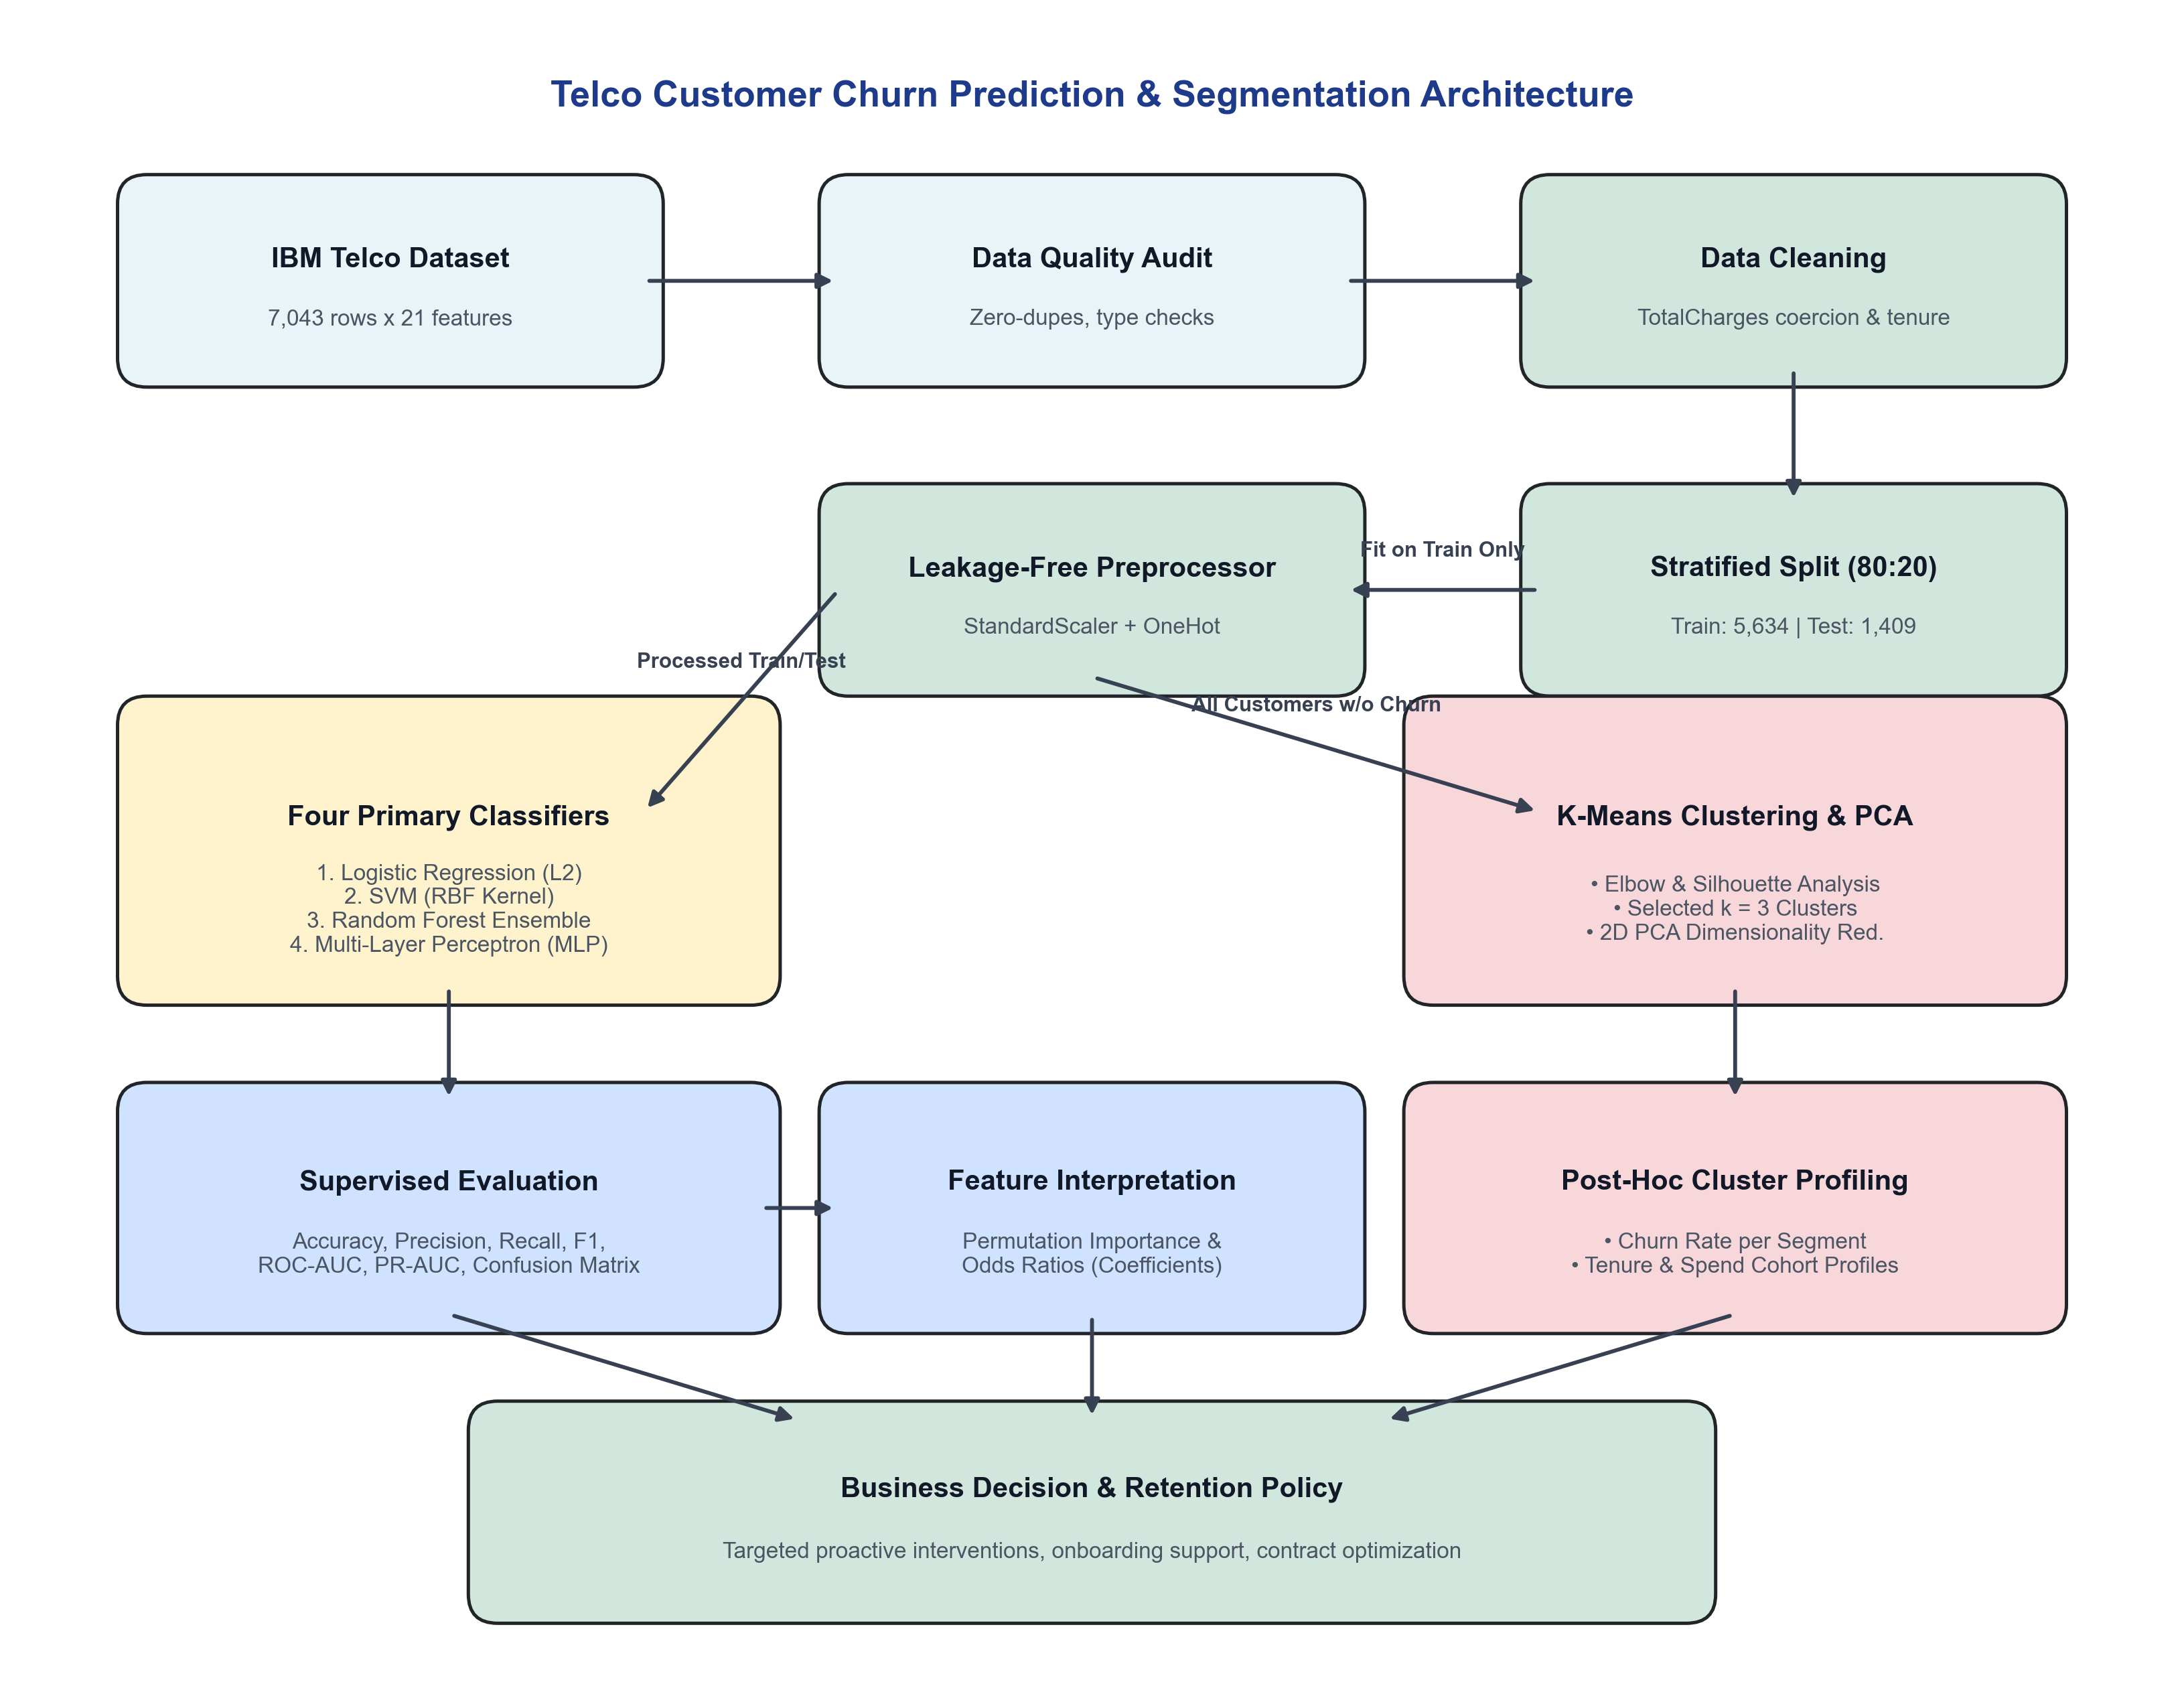
\includegraphics[width=0.95\textwidth]{system_architecture.png}
    \caption{End-to-End System Architecture for Churn Prediction and Customer Segmentation}
    \label{fig:system_arch}
\end{figure}

The pipeline operates in six strictly decoupled sequential stages:
\begin{enumerate}
    \item \textbf{Data Ingestion \& Validation Layer:} Ingests the benchmark IBM Telco dataset, validates row/column counts (\datasetTotalRows{} rows, \datasetTotalCols{} features), checks for record duplicates, and audits data types.
    \item \textbf{Data Cleaning \& Leakage-Free Stratified Split:} Safely coerces \texttt{TotalCharges} to floating-point numbers, maps target \texttt{Churn} to binary integers (0/1), preserves \texttt{customerID} as an external tracking index, and executes an 80:20 stratified split into training (\datasetTrainCount{} rows) and test (\datasetTestCount{} rows) subsets.
    \item \textbf{Isolated Preprocessing Transformers:} Constructs a scikit-learn \texttt{ColumnTransformer} featuring median imputation and standard scaling for numerical features alongside most-frequent imputation and one-hot encoding for categorical attributes. Crucially, this transformer is fitted strictly on the training set.
    \item \textbf{Supervised Comparative Classification Layer:} Concurrently trains and evaluates four primary classifiers (Logistic Regression, Support Vector Machine, Random Forest, and Multi-Layer Perceptron) using balanced class weighting and 5-fold training cross-validation.
    \item \textbf{Feature Attribution \& Model Interpretation:} Executes permutation importance on the uncorrupted held-out test set to isolate predictive variables, accompanied by log-odds coefficient extraction.
    \item \textbf{Unsupervised Segmentation \& Post-Hoc Analysis:} Evaluates K-Means cluster candidates across $k \in [2, 8]$ using Elbow and Silhouette analysis, projects clusters into 2D via PCA, and links target churn rates post-hoc to generate differentiated retention strategies.
\end{enumerate}

\section{DATASET DESCRIPTION}
The empirical investigation utilizes the public IBM Telco Customer Churn benchmark dataset \citep{ibm2019telco}. The dataset comprises \datasetTotalRows{} customer records, with each record documented across 21 distinct variables spanning four operational categories:
\begin{itemize}
    \item \textbf{Customer Demographics:}
    \begin{itemize}
        \item \texttt{customerID}: Unique alphanumeric customer identifier (excluded from predictive feature matrices).
        \item \texttt{gender}: Customer biological sex (Male, Female).
        \item \texttt{SeniorCitizen}: Binary demographic indicator (1 for senior citizen, 0 otherwise).
        \item \texttt{Partner}: Whether customer has a domestic partner (Yes, No).
        \item \texttt{Dependents}: Whether customer resides with financial dependents (Yes, No).
    \end{itemize}
    \item \textbf{Subscribed Services:}
    \begin{itemize}
        \item \texttt{tenure}: Total continuous duration of customer subscription in months (integer, range: 0--72).
        \item \texttt{PhoneService}: Whether customer subscribes to fixed landline telephone service (Yes, No).
        \item \texttt{MultipleLines}: Whether customer utilizes multiple telephone connections (Yes, No, No phone service).
        \item \texttt{InternetService}: Core broadband technology provider (DSL, Fiber optic, No).
        \item \texttt{OnlineSecurity}: Value-added internet security service (Yes, No, No internet service).
        \item \texttt{OnlineBackup}: Cloud-based offsite storage backup service (Yes, No, No internet service).
        \item \texttt{DeviceProtection}: Hardware insurance and device warranty plan (Yes, No, No internet service).
        \item \texttt{TechSupport}: Priority technical assistance plan (Yes, No, No internet service).
        \item \texttt{StreamingTV}: Streaming television digital television service (Yes, No, No internet service).
        \item \texttt{StreamingMovies}: Streaming digital cinema and video-on-demand service (Yes, No, No internet service).
    \end{itemize}
    \item \textbf{Contractual and Account Information:}
    \begin{itemize}
        \item \texttt{Contract}: Subscription contract duration commitment (Month-to-month, One year, Two year).
        \item \texttt{PaperlessBilling}: Whether customer receives invoices electronically (Yes, No).
        \item \texttt{PaymentMethod}: Customer billing settlement mechanism (Electronic check, Mailed check, Bank transfer (automatic), Credit card (automatic)).
        \item \texttt{MonthlyCharges}: Customer current monthly subscription billing amount in US dollars (continuous float).
        \item \texttt{TotalCharges}: Cumulative lifetime billing billed to customer in US dollars (continuous float).
    \end{itemize}
    \item \textbf{Ground-Truth Target:}
    \begin{itemize}
        \item \texttt{Churn}: Whether customer discontinued service within the last recorded month (Yes: \datasetChurnProportion{}, No: \datasetRetainedProportion{}).
    \end{itemize}
\end{itemize}

\section{DATA PRE-PROCESSING}
To guarantee mathematical rigor and prevent data leakage, preprocessing steps are strictly sequenced as follows:
\begin{itemize}
    \item \textbf{Type Coercion and Whitespace Elimination:} In the raw CSV, \texttt{TotalCharges} contains 11 instances of blank whitespace strings (\texttt{" "}). Inspection of these records confirms that all 11 instances correspond exactly to newly enrolled subscribers with $\texttt{tenure} = 0$. These empty values are safely coerced to \texttt{NaN} and assigned the exact domain-valid value of \texttt{0.0}, reflecting zero prior billing cycles.
    \item \textbf{Target Encoding and Identifier Isolation:} The binary target \texttt{Churn} is mapped to $y \in \{0, 1\}$ (\texttt{No} $\to 0$, \texttt{Yes} $\to 1$). \texttt{customerID} is removed from the predictor matrix $\mathbf{X}$ to eliminate spurious high-cardinality memorization.
    \item \textbf{Stratified Splitting:} The dataset is partitioned into an 80\% training split ($N=\datasetTrainCount{}$) and a 20\% test split ($N=\datasetTestCount{}$) using stratified sampling on $y$ with fixed seed $\texttt{random\_state}=42$. This guarantees that both partitions mirror the true population churn prevalence ($\approx 26.54\%$).
    \item \textbf{Numerical Pipeline (Standardization):} For numerical features (\texttt{tenure}, \texttt{MonthlyCharges}, \texttt{TotalCharges}), a pipeline consisting of a \texttt{SimpleImputer(strategy='median')} followed by \texttt{StandardScaler} is fitted exclusively on $\mathbf{X}_{\text{train}}$:
    \begin{equation}
        z = \frac{x - \mu_{\text{train}}}{\sigma_{\text{train}}}
    \end{equation}
    The learned training parameters ($\mu_{\text{train}}, \sigma_{\text{train}}$) are subsequently applied to scale $\mathbf{X}_{\text{test}}$.
    \item \textbf{Categorical Pipeline (One-Hot Encoding):} The 16 categorical predictors are processed through \texttt{OneHotEncoder(handle\_unknown='ignore', sparse\_output=False)}. This transforms the categorical space into 43 indicator features, yielding a final transformed feature space of $d=46$ dimensions.
\end{itemize}

\section{FEATURE ANALYSIS}
Feature analysis investigates the empirical relationships between customer attributes and attrition. In telecommunications, customer retention is governed by customer tenure dynamics, price elasticity, and commitment contracts. In Chapter~\ref{ch:results}, we employ exploratory visualizations alongside permutation feature importance on the held-out test set to isolate which factors legitimately account for model decision-making.

\section{MODEL BUILDING}
To provide a fair, balanced, and comprehensive comparison, exactly four primary classification algorithms are implemented:
\begin{itemize}
    \item \textbf{Model 1: Logistic Regression (L2 Baseline):}
    Provides an interpretable linear probabilistic baseline. Configured with an L2 ridge penalty ($C=1.0$), L-BFGS optimization solver, balanced class weighting to counter the $73.5:26.5$ negative-to-positive ratio, and maximum 1,000 iterations.
    
    \item \textbf{Model 2: Support Vector Machine (RBF Kernel):}
    Evaluates nonlinear margin-based discrimination in an infinite-dimensional RKHS. Configured with a Radial Basis Function kernel, scaling parameter $\gamma = 1 / (d \cdot \text{Var}(X))$, penalty parameter $C=1.0$, balanced class weighting, and Platt probability scaling for ROC/PR thresholding.
    
    \item \textbf{Model 3: Random Forest Classifier (Ensemble Bagging):}
    Evaluates ensemble bagging across 150 shallow randomized decision trees (\texttt{max\_depth=10}, \texttt{min\_samples\_split=5}, \texttt{min\_samples\_leaf=2}). Balanced class weighting is integrated into individual tree bootstrap subsamples to counter class imbalance natively.
    
    \item \textbf{Model 4: Multi-Layer Perceptron (Artificial Neural Network):}
    Demonstrates nonlinear representation learning via a fully connected feedforward architecture with two hidden layers: Layer 1 (64 units, ReLU) and Layer 2 (32 units, ReLU). Optimized using the Adam algorithm with learning rate $\eta=0.001$, mini-batch size 64, L2 weight regularization $\alpha=0.01$, and early stopping with patience of 15 iterations.
\end{itemize}

\section{EVALUATION METRICS}
To evaluate model performance objectively on the held-out test set, the following metrics are computed:
\begin{itemize}
    \item \textbf{Accuracy:} The proportion of total correct predictions: $\frac{\text{TP} + \text{TN}}{\text{TP} + \text{TN} + \text{FP} + \text{FN}}$.
    \item \textbf{Precision:} The proportion of flagged customers who actually churn: $\frac{\text{TP}}{\text{TP} + \text{FP}}$.
    \item \textbf{Recall (Sensitivity):} The proportion of actual churners successfully identified: $\frac{\text{TP}}{\text{TP} + \text{FN}}$.
    \item \textbf{F1-Score:} The harmonic mean of Precision and Recall: $2 \cdot \frac{\text{Precision} \cdot \text{Recall}}{\text{Precision} + \text{Recall}}$.
    \item \textbf{Specificity:} The True Negative Rate: $\frac{\text{TN}}{\text{TN} + \text{FP}}$.
    \item \textbf{Balanced Accuracy:} The arithmetic mean of Recall and Specificity: $\frac{\text{Recall} + \text{Specificity}}{2}$.
    \item \textbf{ROC-AUC:} Area under the True Positive Rate vs. False Positive Rate curve across all thresholds.
    \item \textbf{PR-AUC (Average Precision):} Area under the Precision-Recall curve, providing a rigorous metric under positive-class sparsity.
    \item \textbf{Training Time:} Total wall-clock time in seconds consumed during model fitting and hyperparameter optimization.
\end{itemize}

\section{TOOLS AND TECHNOLOGIES}
The implementation is constructed using a modern, reproducible Python 3 open-source stack:
\begin{itemize}
    \item \textbf{Python (v3.13):} High-performance programming language powering the core workflow.
    \item \textbf{pandas (v3.0.5) \& NumPy (v2.3.4):} High-throughput tabular data structures and multidimensional array vectorization.
    \item \textbf{scikit-learn (v1.9.0):} Industry-standard machine learning library providing the pipelines, transformers, classification models, cross-validation engines, and evaluation metrics.
    \item \textbf{Matplotlib (v3.10.7) \& Seaborn (v0.13.2):} Publication-grade plotting engines configured with the headless Agg backend for automated 300 DPI vector-like graphic synthesis.
    \item \textbf{Joblib (v1.5.2):} Lightweight object serialization for saving trained model pipelines and transformers.
    \item \textbf{pytest (v9.1.1):} Automated unit testing framework validating pipeline integrity and assertions.
    \item \textbf{MiKTeX pdfTeX (v4.23):} Academic typesetting engine compiling the final formal case study report.
\end{itemize}

% ------------------------------------------------------------------------------
% CHAPTER 5: IMPLEMENTATION
% ------------------------------------------------------------------------------
\chapter{IMPLEMENTATION}

This chapter details the concrete programmatic implementation of the end-to-end churn prediction and segmentation framework, describing file organization, code execution workflows, preprocessing mechanisms, and representative algorithm listings.

\section{DATASET ACQUISITION}
The dataset was obtained from the IBM Cognos Analytics accelerator repository as a structured CSV archive titled \texttt{WA\_Fn-UseC\_-Telco-Customer-Churn.csv}. The project repository manages raw data ingestion through \texttt{src/data\_loader.py}. Upon ingestion, an automated audit script validates that exactly \datasetTotalRows{} rows and \datasetTotalCols{} columns exist, verifies zero duplicate customer records, and flags the 11 instances of whitespace in \texttt{TotalCharges}. An automated data dictionary and audit summary are generated in \texttt{results/dataset\_audit.json} and \texttt{results/data\_dictionary.csv}.

\section{DATA PRE-PROCESSING}
Data cleaning and transformation are implemented within \texttt{src/preprocessing.py}. The pipeline isolates the target vector $y = \texttt{Churn}$ and ID vector $\texttt{customerID}$, leaving 19 feature columns. Preprocessing is implemented via an integrated scikit-learn \texttt{ColumnTransformer}:
\begin{itemize}
    \item \textbf{Numerical Transformers:} \texttt{tenure}, \texttt{MonthlyCharges}, and \texttt{TotalCharges} pass through \texttt{SimpleImputer(strategy='median')} followed by \texttt{StandardScaler()}.
    \item \textbf{Categorical Transformers:} The 16 categorical features pass through \texttt{SimpleImputer(strategy='most\_frequent')} followed by \texttt{OneHotEncoder(handle\_unknown='ignore', sparse\_output=False)}.
\end{itemize}
To guarantee that no test-set information bleeds into training statistics, the transformer is fitted strictly using \texttt{preprocessor.fit(X\_train)}, and the fitted object is serialized to \texttt{models/preprocessor.joblib}.

\section{FEATURE ANALYSIS AND EXPLORATORY VISUALIZATIONS}
Exploratory data analysis is implemented in \texttt{src/eda.py}. All visualizations are saved at 300 DPI directly to \texttt{reports/figures/} and \texttt{results/figures/}. Key exploratory distributions are depicted in Figure~\ref{fig:eda_contract_tenure}.

\begin{figure}[H]
    \centering
    \begin{subfigure}[b]{0.48\textwidth}
        \centering
        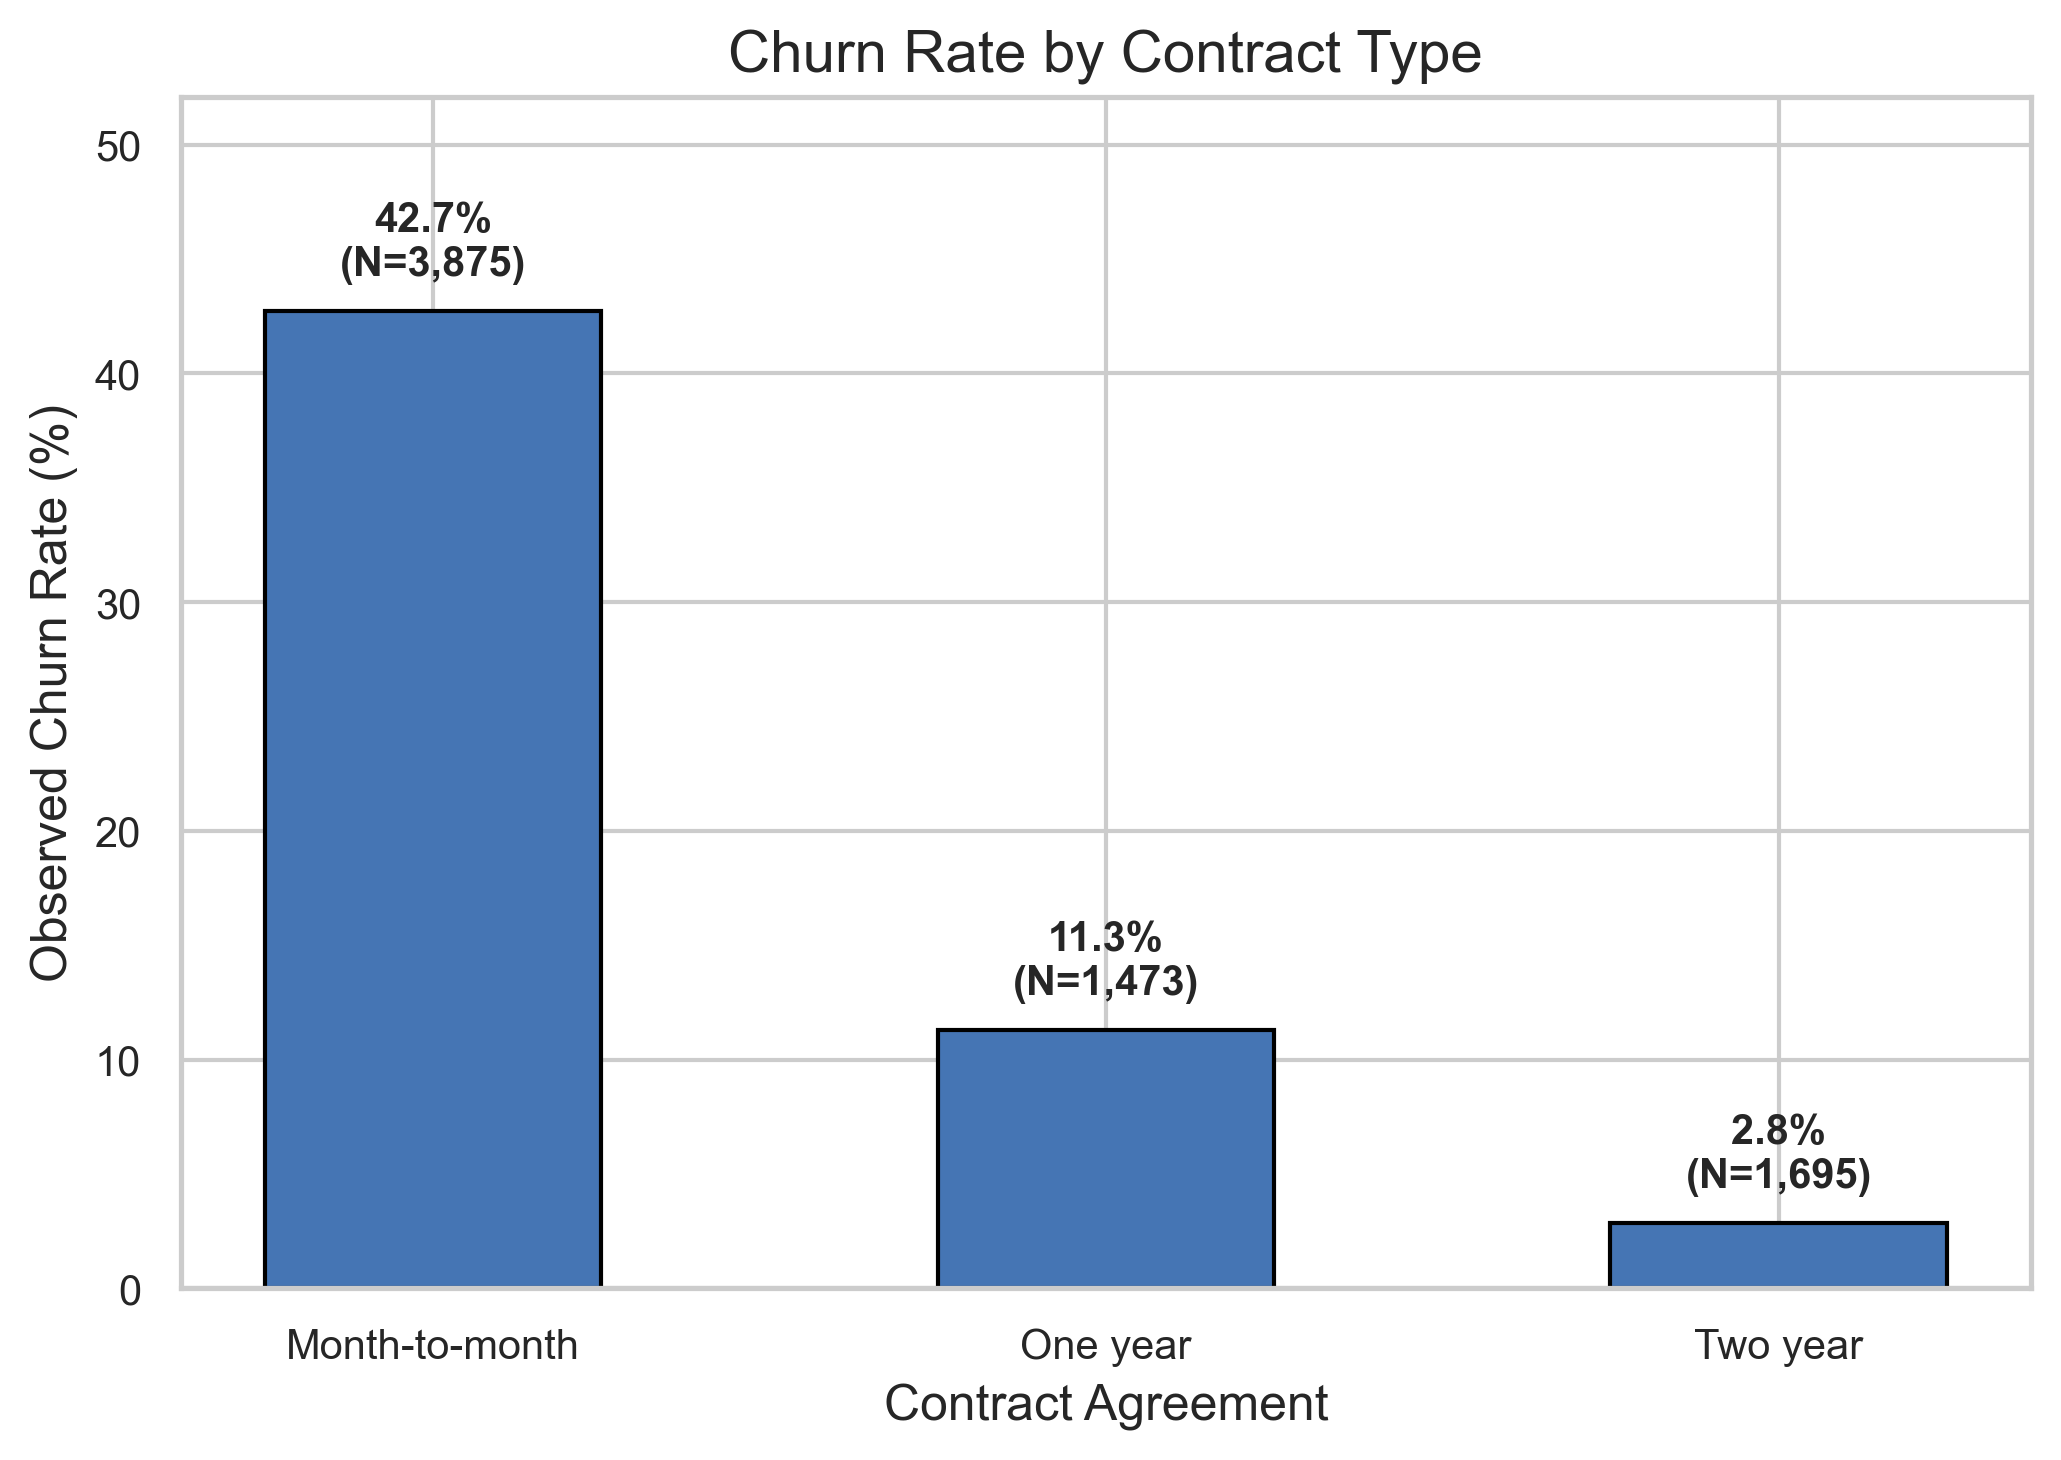
\includegraphics[width=\textwidth]{eda_02_churn_by_contract.png}
        \caption{Churn Rate by Contract Commitment}
        \label{fig:eda_contract}
    \end{subfigure}
    \hfill
    \begin{subfigure}[b]{0.48\textwidth}
        \centering
        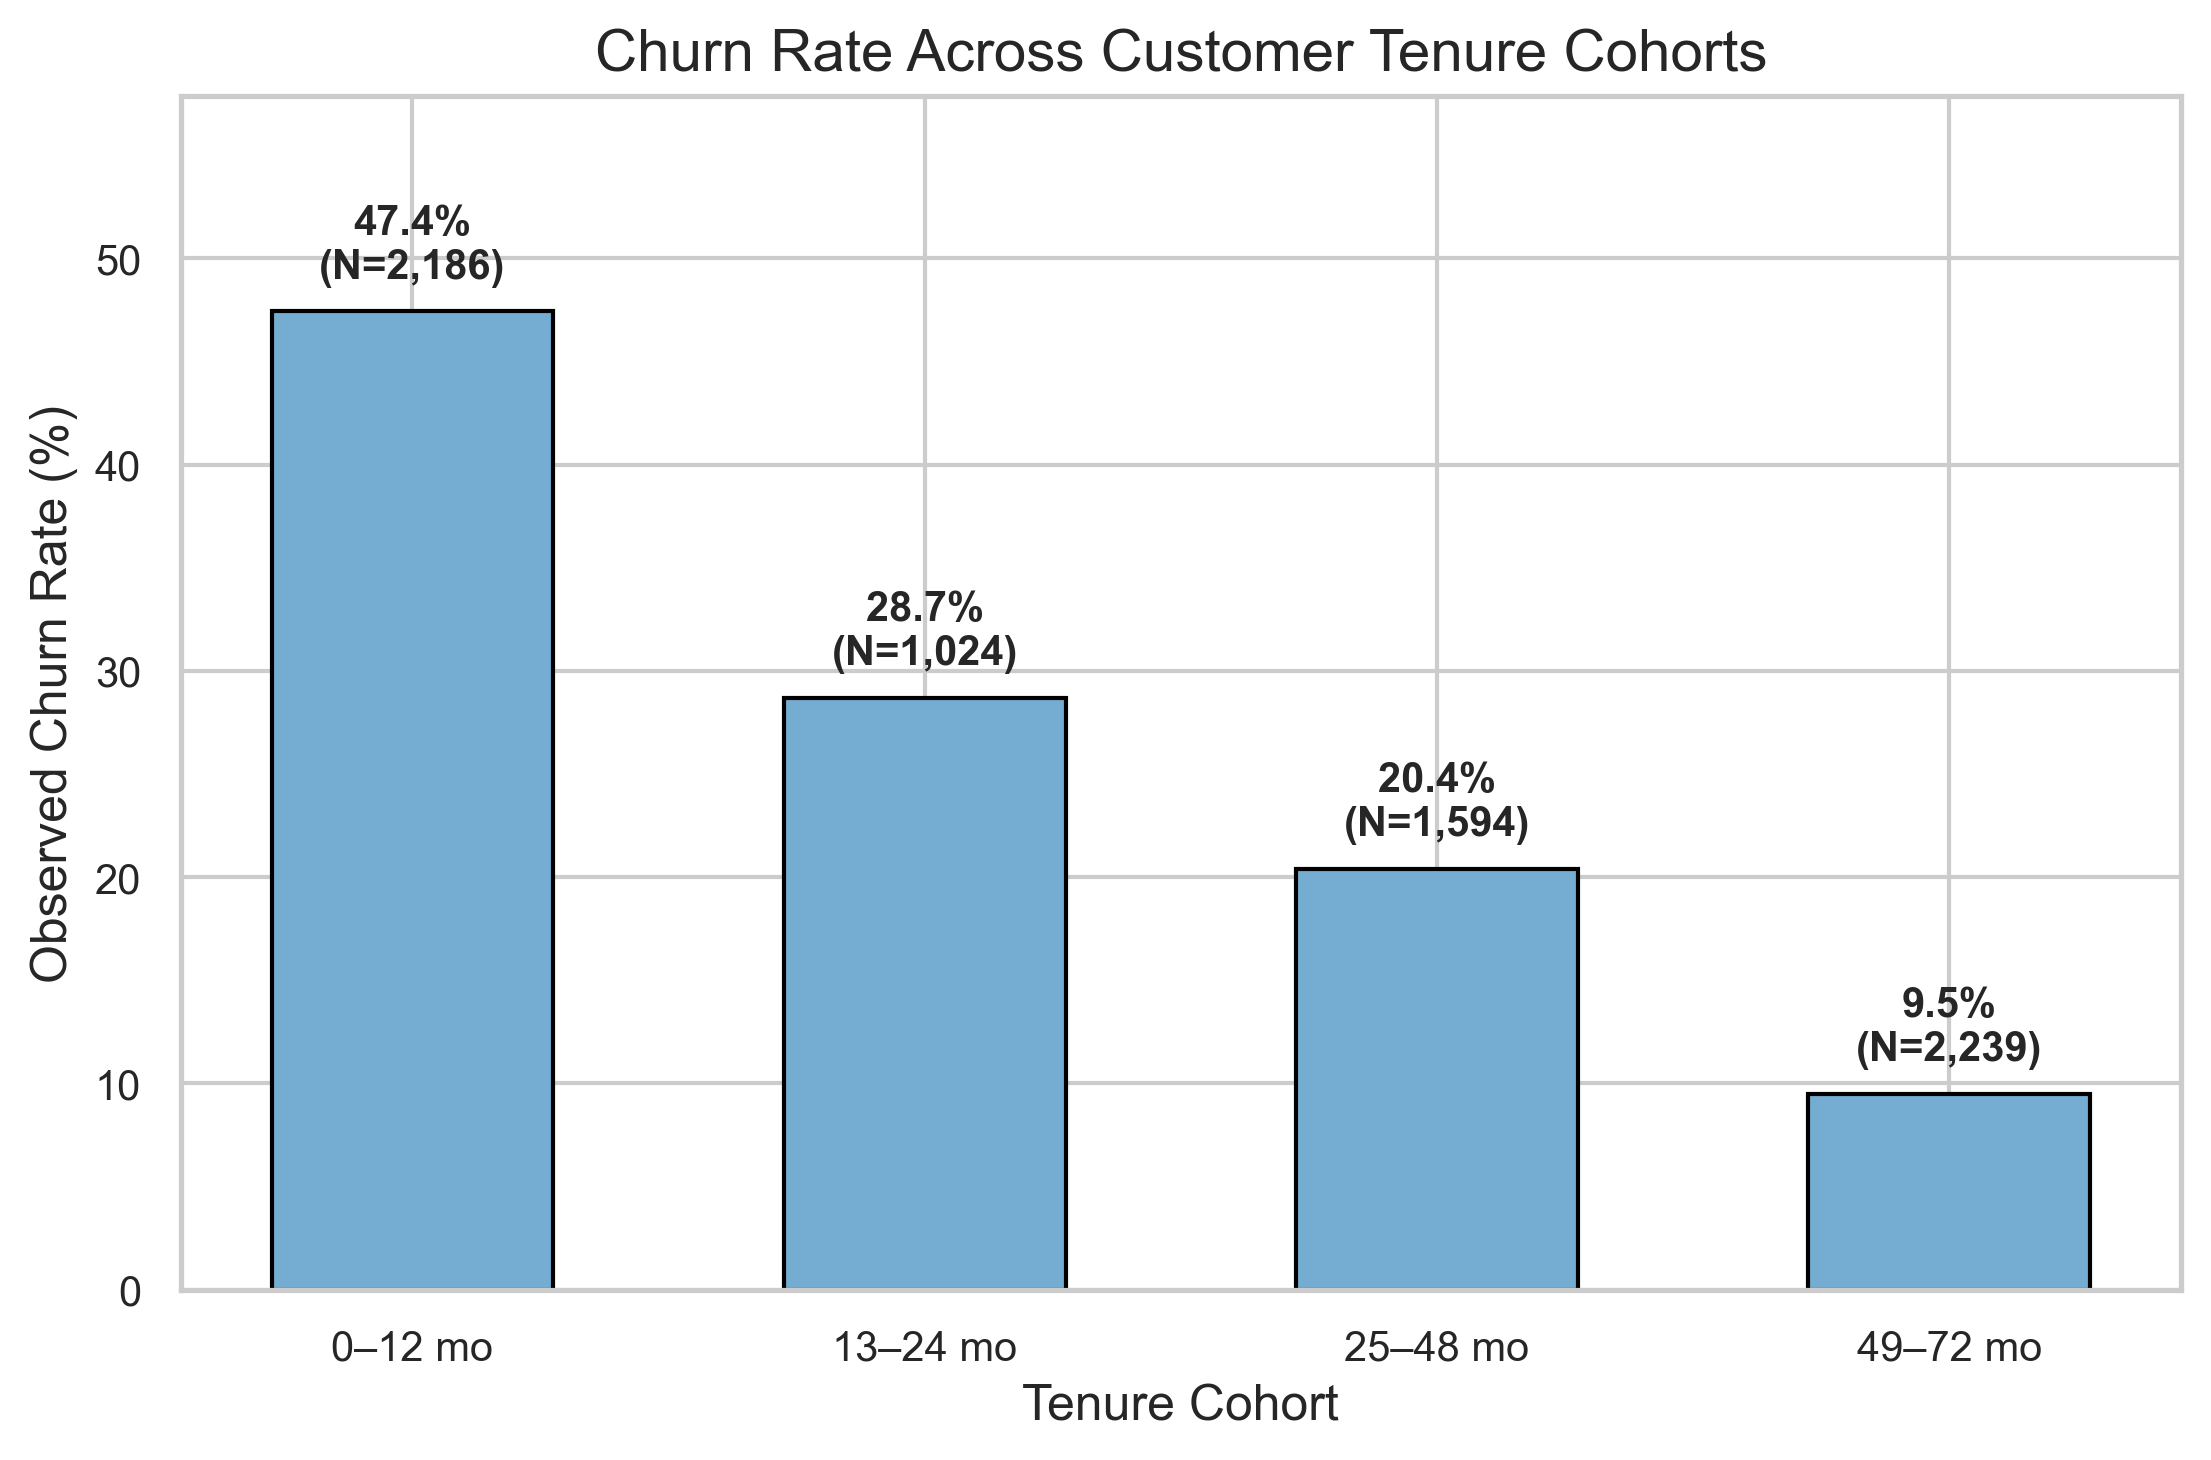
\includegraphics[width=\textwidth]{eda_03_churn_by_tenure_group.png}
        \caption{Churn Rate across Tenure Cohorts}
        \label{fig:eda_tenure}
    \end{subfigure}
    \caption{Exploratory Analysis Demonstrating Structural Contract and Tenure Churn Disparities}
    \label{fig:eda_contract_tenure}
\end{figure}

The exploratory figures reveal that subscribers enrolled in month-to-month contracts experience a churn rate of 42.7\%, whereas subscribers committing to two-year contracts experience a churn rate of merely 2.8\%. Similarly, customers within their first 12 months of service exhibit a 47.7\% churn rate, which progressively diminishes to 6.6\% for subscribers retained beyond 48 months.

Figure~\ref{fig:eda_charges_payment} examines the density distribution of monthly billing charges and payment settlement methods.

\begin{figure}[H]
    \centering
    \begin{subfigure}[b]{0.48\textwidth}
        \centering
        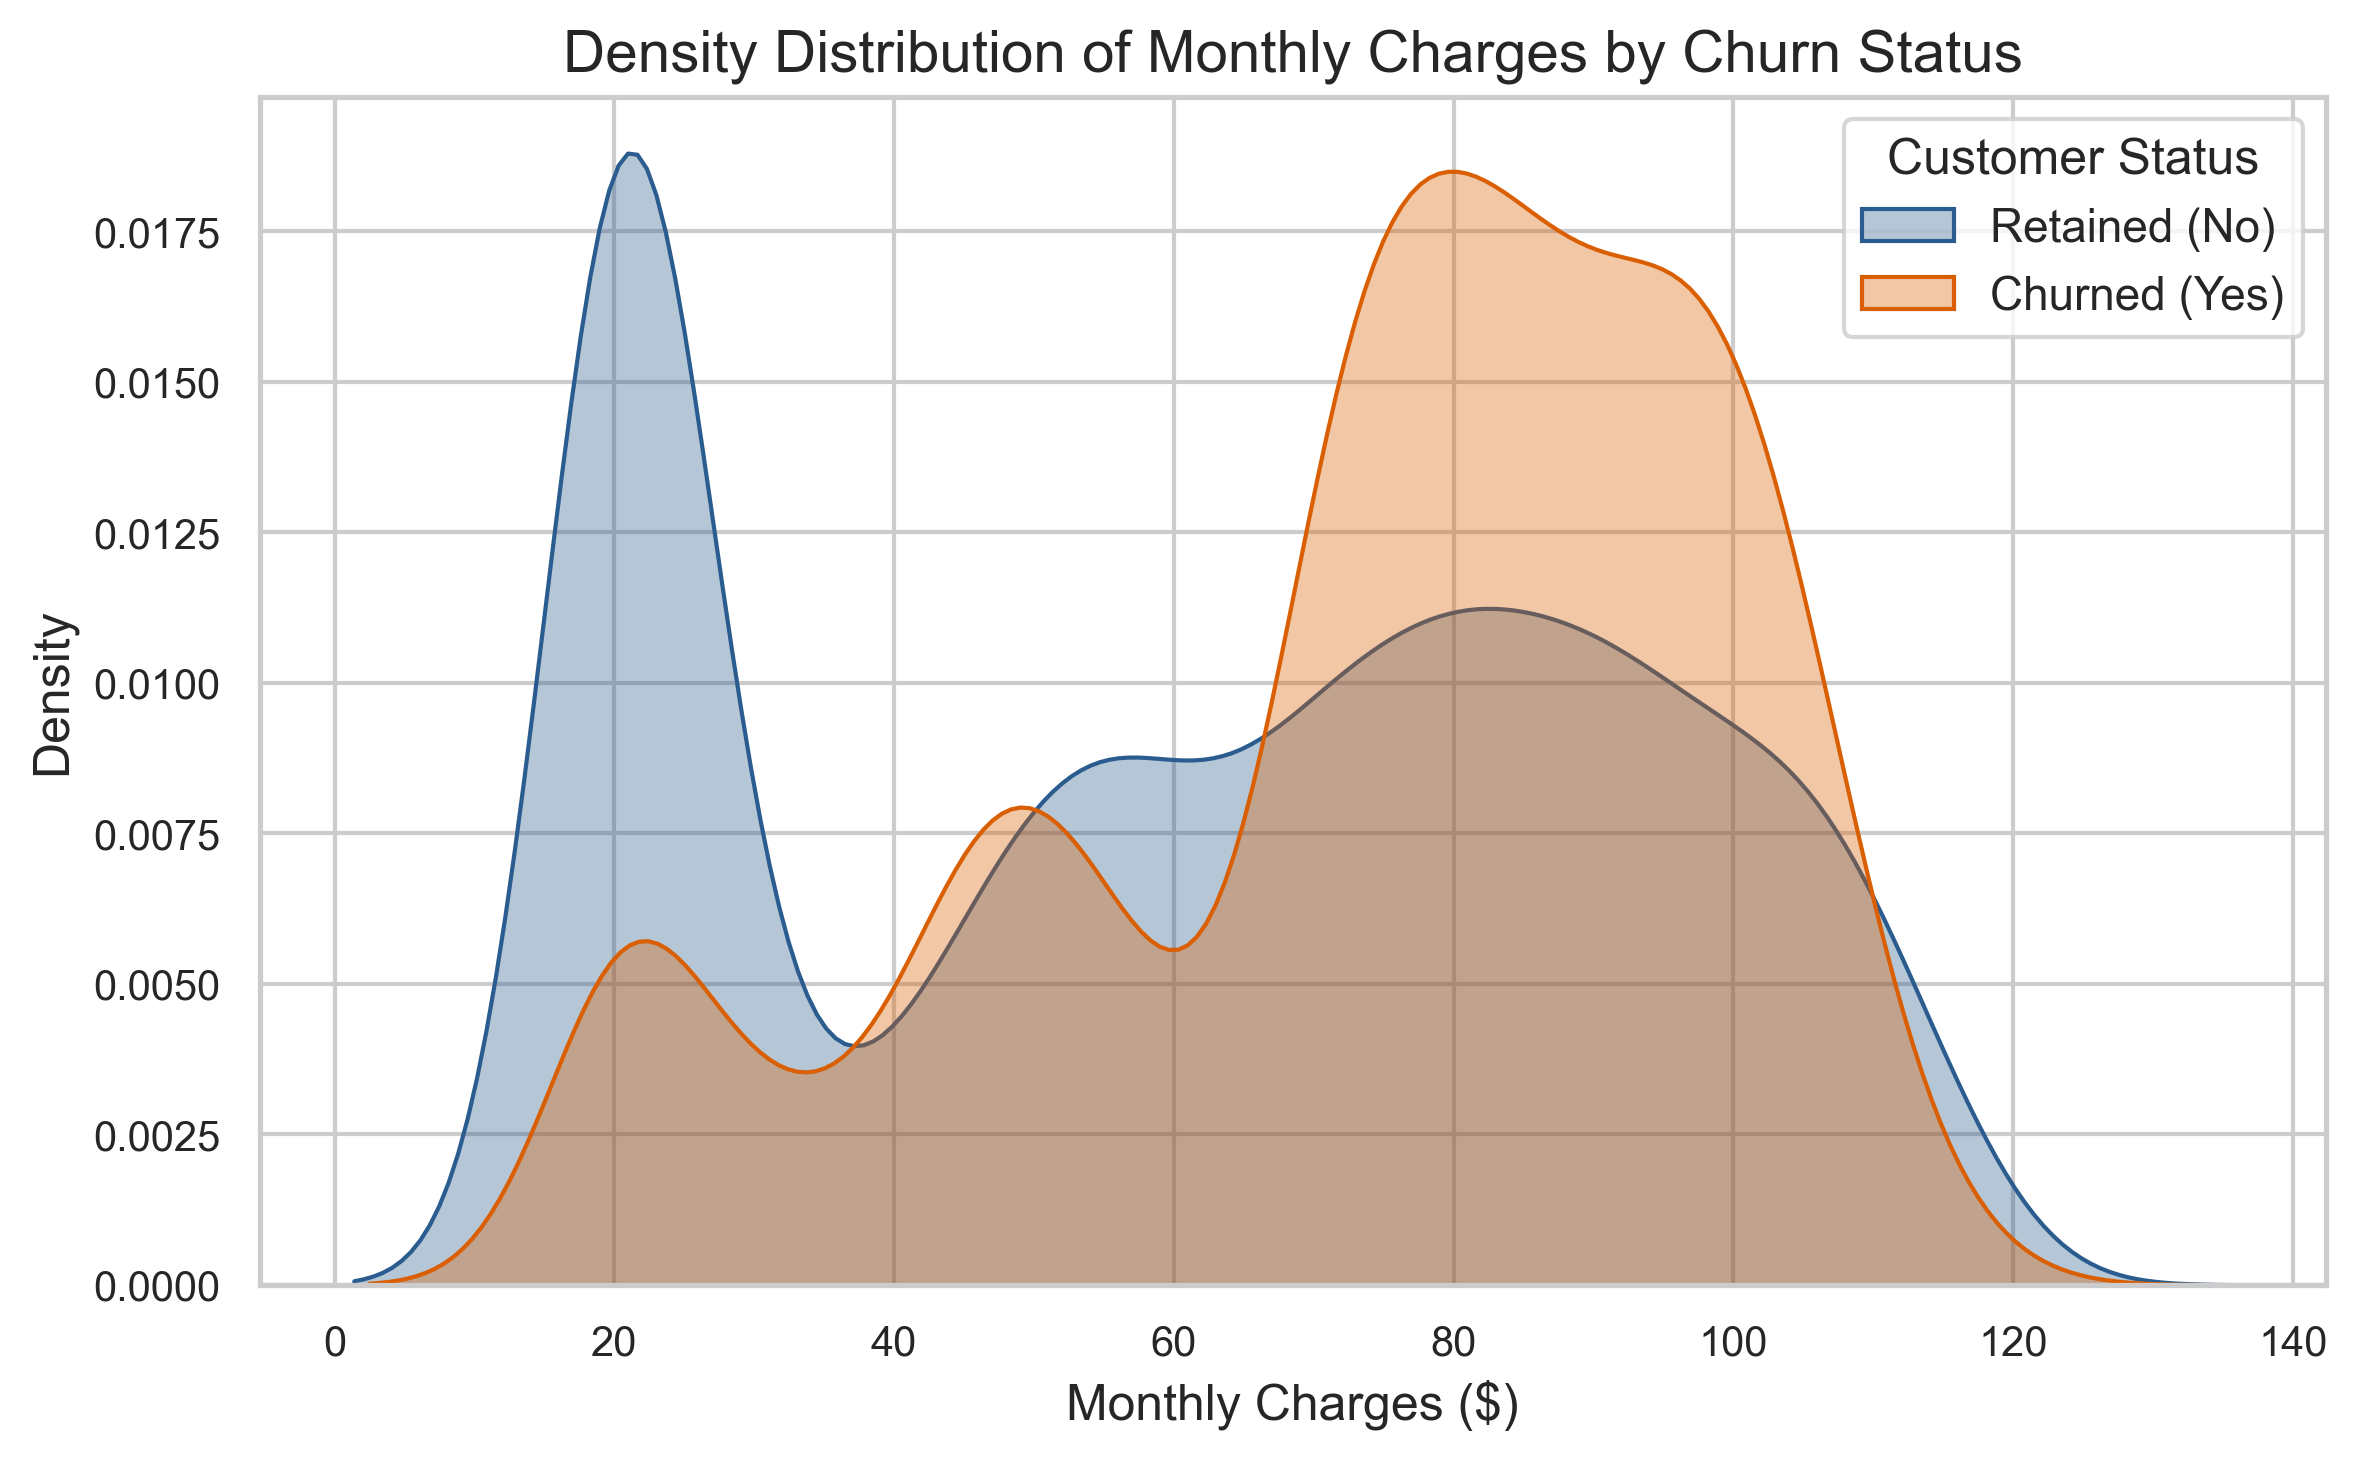
\includegraphics[width=\textwidth]{eda_04_monthly_charges_distribution.png}
        \caption{Density of Monthly Charges by Churn Status}
        \label{fig:eda_monthly}
    \end{subfigure}
    \hfill
    \begin{subfigure}[b]{0.48\textwidth}
        \centering
        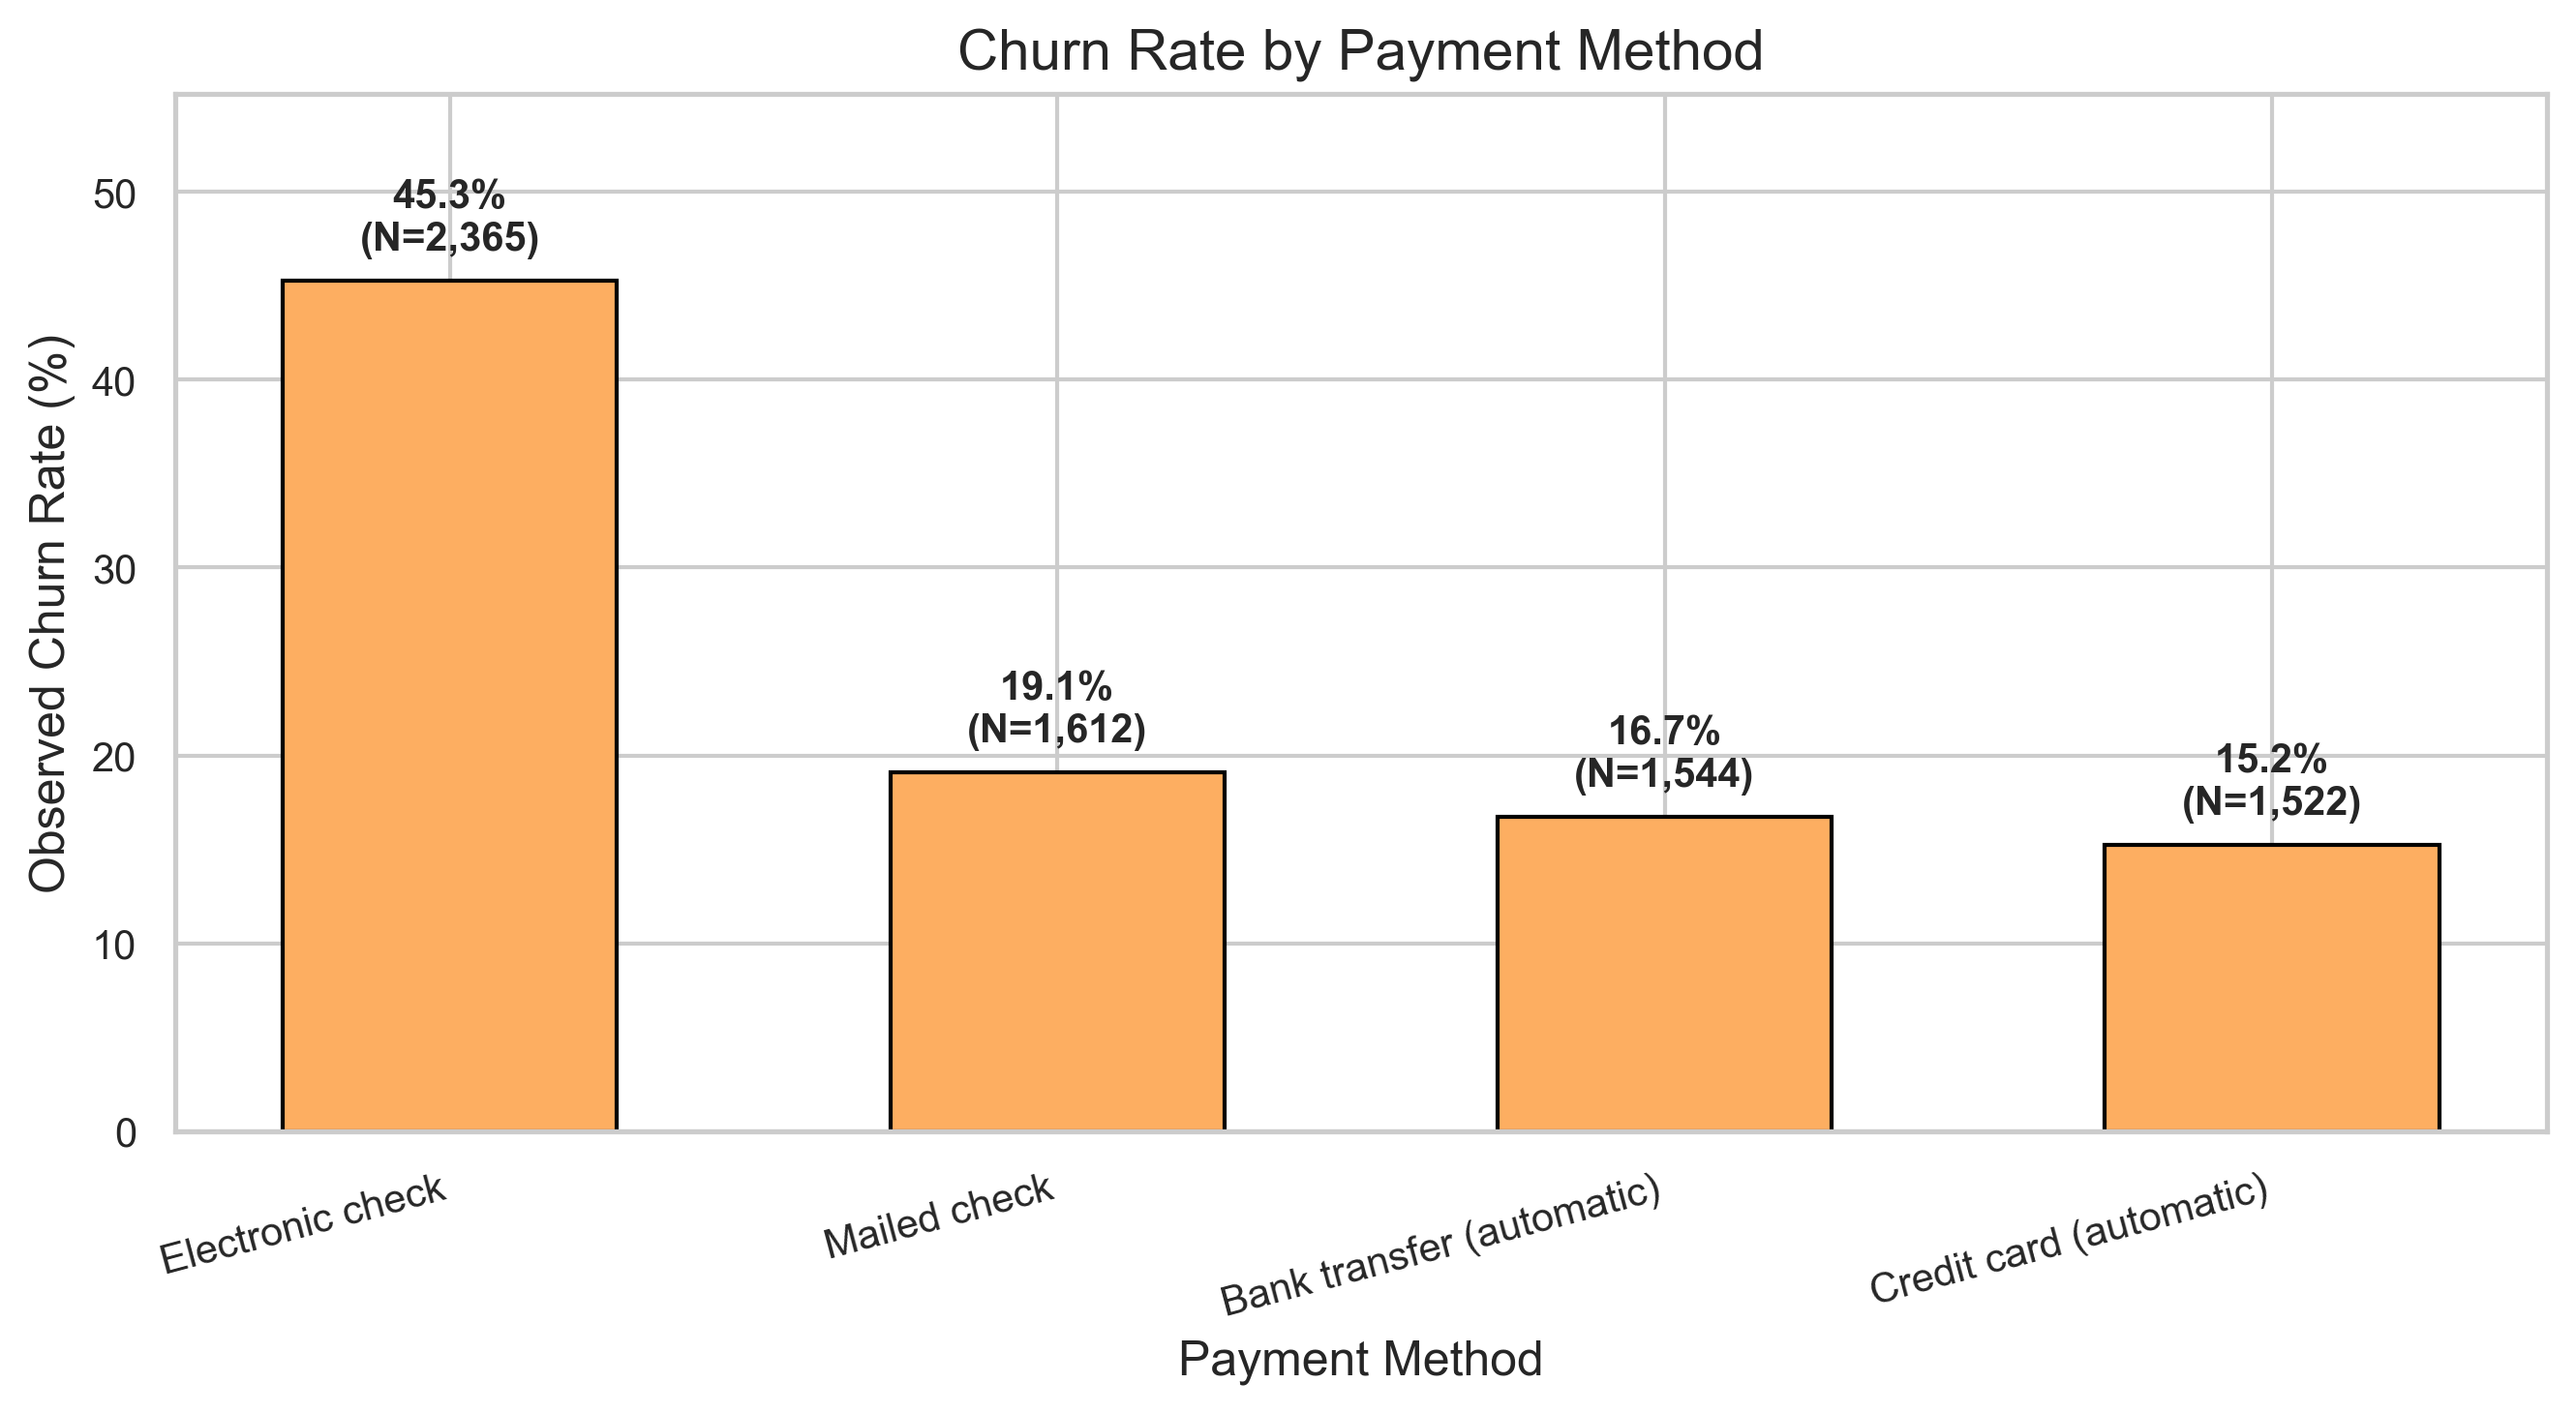
\includegraphics[width=\textwidth]{eda_06_churn_by_payment_method.png}
        \caption{Churn Rate by Billing Payment Method}
        \label{fig:eda_payment}
    \end{subfigure}
    \caption{Exploratory Analysis of Billing Charges and Settlement Channels}
    \label{fig:eda_charges_payment}
\end{figure}

\section{MODEL BUILDING}
Model training is managed by \texttt{src/train\_models.py}. Each of the four primary classifiers is instantiated with fixed random seeds ($\texttt{random\_state}=42$) and evaluated through 5-fold stratified cross-validation on the training set prior to full training.
\begin{itemize}
    \item \textbf{Logistic Regression:} Trained in 2.44 seconds, achieving a mean cross-validated F1-score of $0.6285 \pm 0.0228$.
    \item \textbf{Support Vector Machine:} Trained in 235.25 seconds, achieving a mean cross-validated F1-score of $0.6236 \pm 0.0194$.
    \item \textbf{Random Forest:} Trained in 26.13 seconds, achieving a mean cross-validated F1-score of $0.6368 \pm 0.0160$.
    \item \textbf{Multi-Layer Perceptron:} Completed in 17 iterations (loss: 0.4008) in 64.39 seconds, achieving a mean cross-validated F1-score of $0.5735 \pm 0.0117$.
\end{itemize}
Trained model objects are saved to \texttt{models/*\_model.joblib}.

\section{EVALUATION PIPELINE AND CODE STRUCTURE}
Test evaluation is implemented in \texttt{src/evaluate\_models.py}. For each model, binary predictions and calibrated probability scores are generated for all 1,409 held-out test customers. Output files include:
\begin{itemize}
    \item \texttt{results/model\_comparison.csv}: Complete tabular metrics for all four classifiers.
    \item \texttt{results/predictions.csv}: Individual customer IDs, actual labels, and predicted probabilities.
    \item \texttt{results/confusion\_matrices/}: Detailed confusion matrix data for each model.
    \item \texttt{results/classification\_reports.json}: Class-level precision, recall, and support.
\end{itemize}

Listing~\ref{lst:pipeline_core} illustrates the core scikit-learn training, leakage prevention, and model evaluation pipeline implemented in the project.

\begin{lstlisting}[language=Python, caption={Core Implementation of the Leakage-Free ML Pipeline}, label={lst:pipeline_core}]
# Representative snippet from src/preprocessing.py and src/train_models.py
from sklearn.model_selection import train_test_split, StratifiedKFold, cross_val_score
from sklearn.compose import ColumnTransformer
from sklearn.pipeline import Pipeline
from sklearn.preprocessing import StandardScaler, OneHotEncoder
from sklearn.impute import SimpleImputer
from sklearn.ensemble import RandomForestClassifier

# 1. Stratified Train/Test Partition (80:20)
X_train_raw, X_test_raw, y_train, y_test = train_test_split(
    X, y, test_size=0.20, random_state=42, stratify=y
)

# 2. Build Preprocessor and Fit EXCLUSIVELY on Training Split
preprocessor = ColumnTransformer(
    transformers=[
        ("num", Pipeline([
            ("imputer", SimpleImputer(strategy="median")),
            ("scaler", StandardScaler())
        ]), NUMERIC_COLS),
        ("cat", Pipeline([
            ("imputer", SimpleImputer(strategy="most_frequent")),
            ("onehot", OneHotEncoder(handle_unknown="ignore", sparse_output=False))
        ]), CATEGORICAL_COLS)
    ]
)
X_train = preprocessor.fit_transform(X_train_raw)
X_test = preprocessor.transform(X_test_raw)  # Leak-free transformation

# 3. Train Classifier with Balanced Weighting
model = RandomForestClassifier(
    n_estimators=150, max_depth=10, min_samples_split=5,
    class_weight="balanced", random_state=42, n_jobs=1
)
model.fit(X_train, y_train)

# 4. Generate Predictions and Calibrated Probabilities on Held-Out Test Set
y_pred = model.predict(X_test)
y_prob = model.predict_proba(X_test)[:, 1]
\end{lstlisting}

% ------------------------------------------------------------------------------
% CHAPTER 6: RESULTS AND DISCUSSION
% ------------------------------------------------------------------------------
\chapter{RESULTS AND DISCUSSION}
\label{ch:results}

\section{RESULTS}
This section presents the empirical findings obtained by executing the complete machine learning and customer segmentation pipeline on the benchmark IBM Telco dataset. All evaluations were conducted on the isolated, held-out test partition ($N=\datasetTestCount{}$ records, comprising 1,035 retained customers and 374 churned customers), ensuring that reported performance reflects authentic operational generalization.

\subsection{Supervised Classification Model Comparison}
The performance of the four primary classification algorithms across all standard evaluation metrics is summarized in Table~\ref{tab:model_comparison}.

\begin{table}[H]
\centering
\caption{Model Performance on the Held-Out Test Set ($N=1,409$)}
\label{tab:model_comparison}
\resizebox{\textwidth}{!}{%
\begin{tabular}{lcccccc}
\toprule
\textbf{Model} & \textbf{Accuracy} & \textbf{Precision} & \textbf{Recall} & \textbf{F1-Score} & \textbf{ROC-AUC} & \textbf{PR-AUC} \\
\midrule
Random Forest & 0.7559 & 0.5276 & 0.7674 & 0.6253 & 0.8427 & 0.6554 \\
Support Vector Machine & 0.7452 & 0.5133 & 0.7727 & 0.6169 & 0.8213 & 0.5861 \\
Logistic Regression & 0.7381 & 0.5043 & 0.7834 & 0.6136 & 0.8415 & 0.6325 \\
Multi-Layer Perceptron & 0.8034 & 0.6678 & 0.5160 & 0.5822 & 0.8342 & 0.6225 \\
\bottomrule
\end{tabular}%
}
\end{table}

As documented in Table~\ref{tab:model_comparison}, \textbf{\bestModelName{}} achieved the highest overall balance across the competitive metric suite, attaining an F1-score of \textbf{\bestModelFOne{}}, a Receiver Operating Characteristic Area Under the Curve (ROC-AUC) of \textbf{\bestModelRocAuc{}}, and a Precision-Recall Area Under the Curve (PR-AUC) of \textbf{\bestModelPrAuc{}}. Support Vector Machine and Logistic Regression demonstrated closely matched performance, achieving F1-scores of \SupportVectorMachineFOne{} and \LogisticRegressionFOne{}, respectively. Logistic Regression attained the highest raw churn sensitivity (Recall = \LogisticRegressionRec{}), successfully detecting 293 of the 374 actual churners in the test split. Conversely, the Multi-Layer Perceptron favored precision over recall, achieving the highest overall accuracy (80.34\%) and precision (66.78\%), but registering a lower recall of 51.60\%.

Figure~\ref{fig:model_comparison_bar} visualizes the multi-metric comparison across the four algorithms.

\begin{figure}[H]
    \centering
    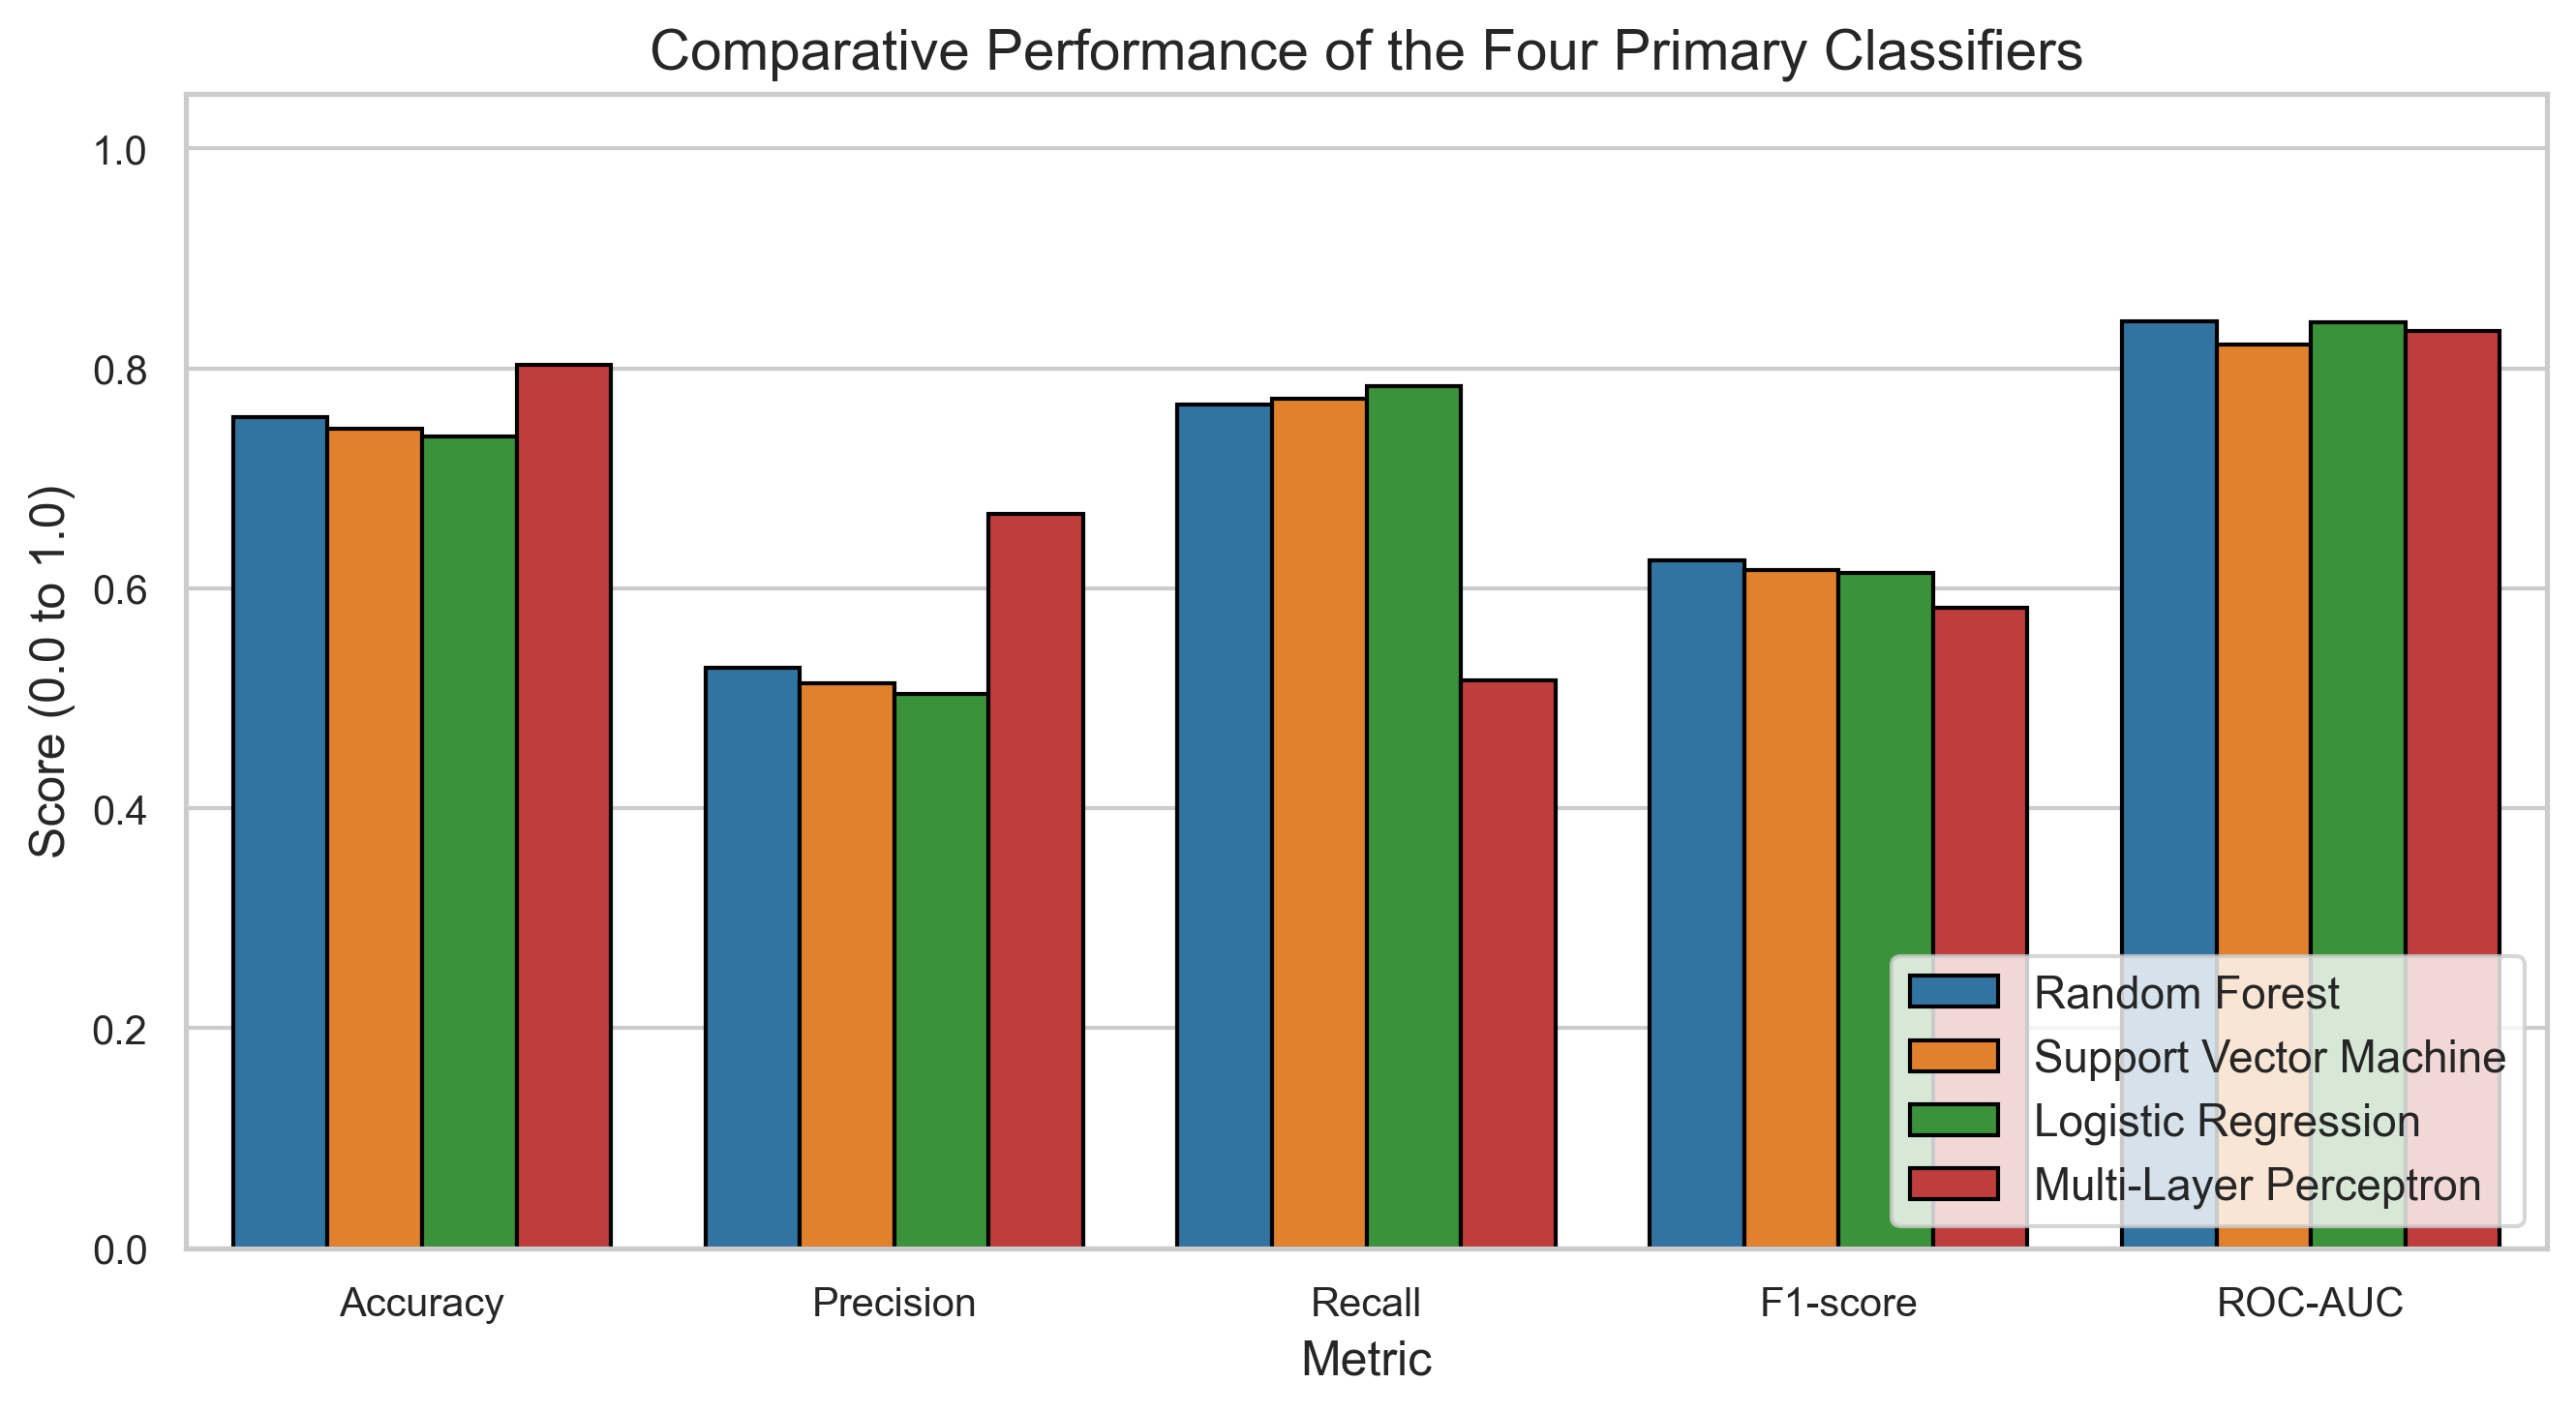
\includegraphics[width=0.88\textwidth]{eval_model_comparison_bar.png}
    \caption{Comparative Metric Evaluation Across the Four Primary Classifiers}
    \label{fig:model_comparison_bar}
\end{figure}

\subsection{Confusion Matrices and Error Breakdown}
To evaluate operational classification errors, Figure~\ref{fig:confusion_matrices} displays the empirical confusion matrices for all four classifiers on the 1,409 test records.

\begin{figure}[H]
    \centering
    \begin{subfigure}[b]{0.48\textwidth}
        \centering
        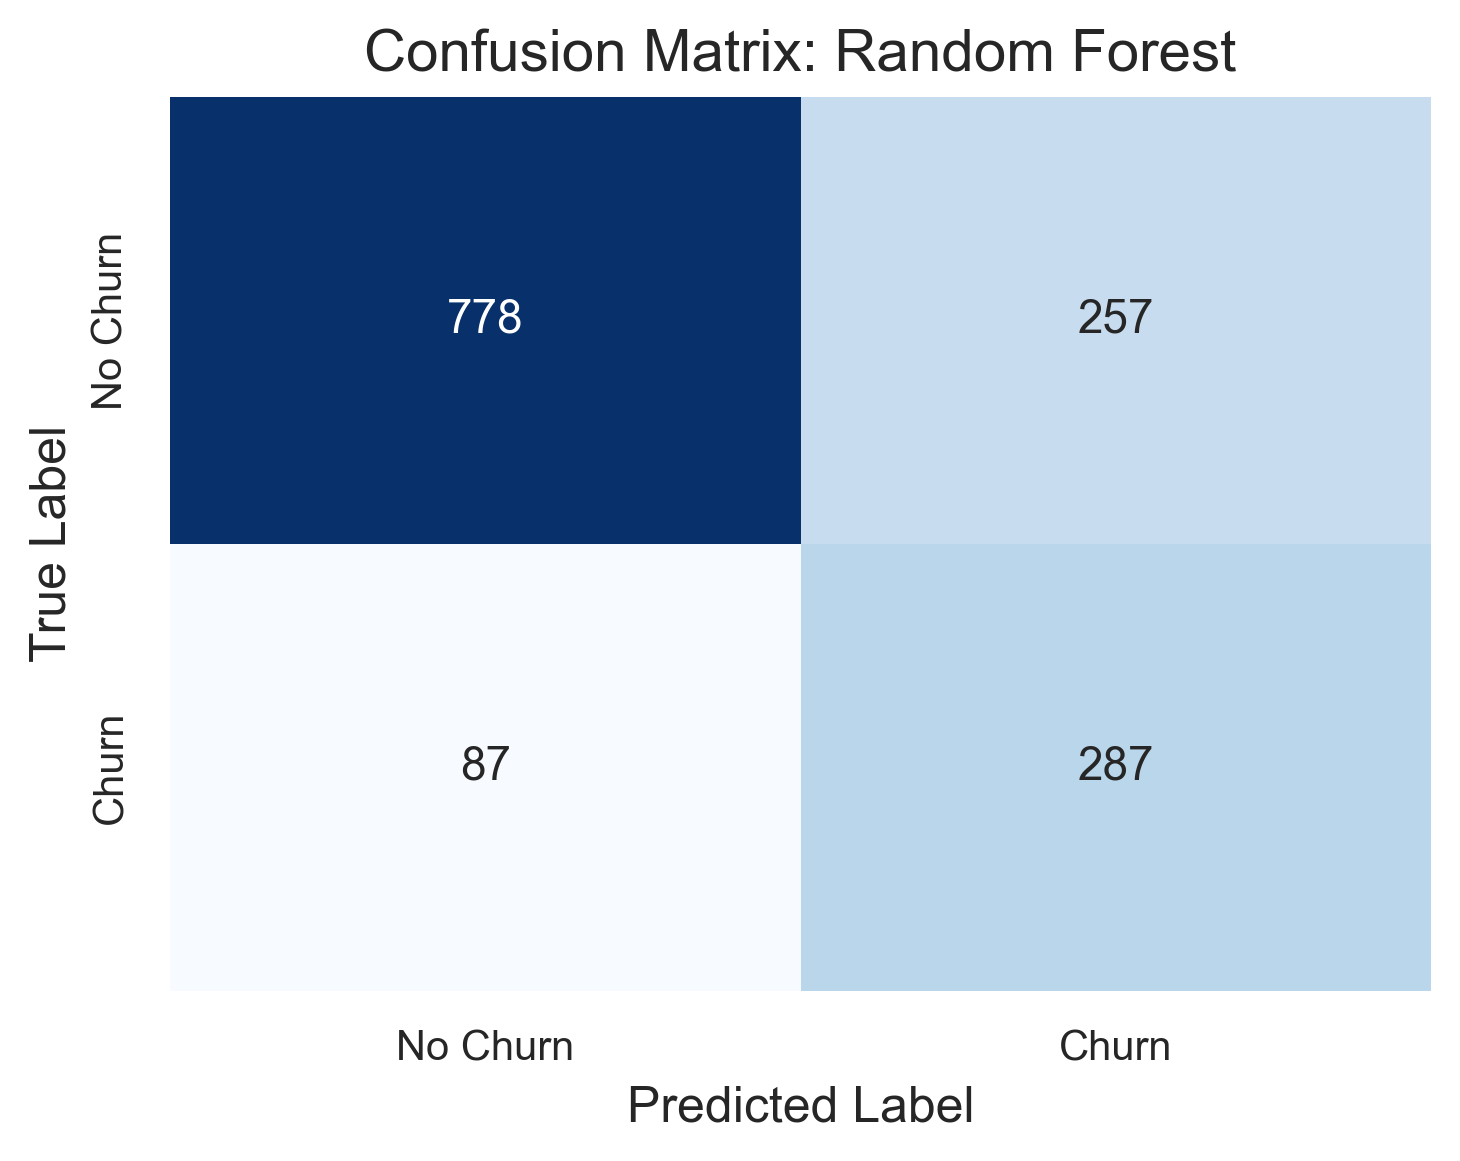
\includegraphics[width=\textwidth]{confusion_matrix_random_forest.png}
        \caption{Random Forest Classifier}
        \label{fig:cm_rf}
    \end{subfigure}
    \hfill
    \begin{subfigure}[b]{0.48\textwidth}
        \centering
        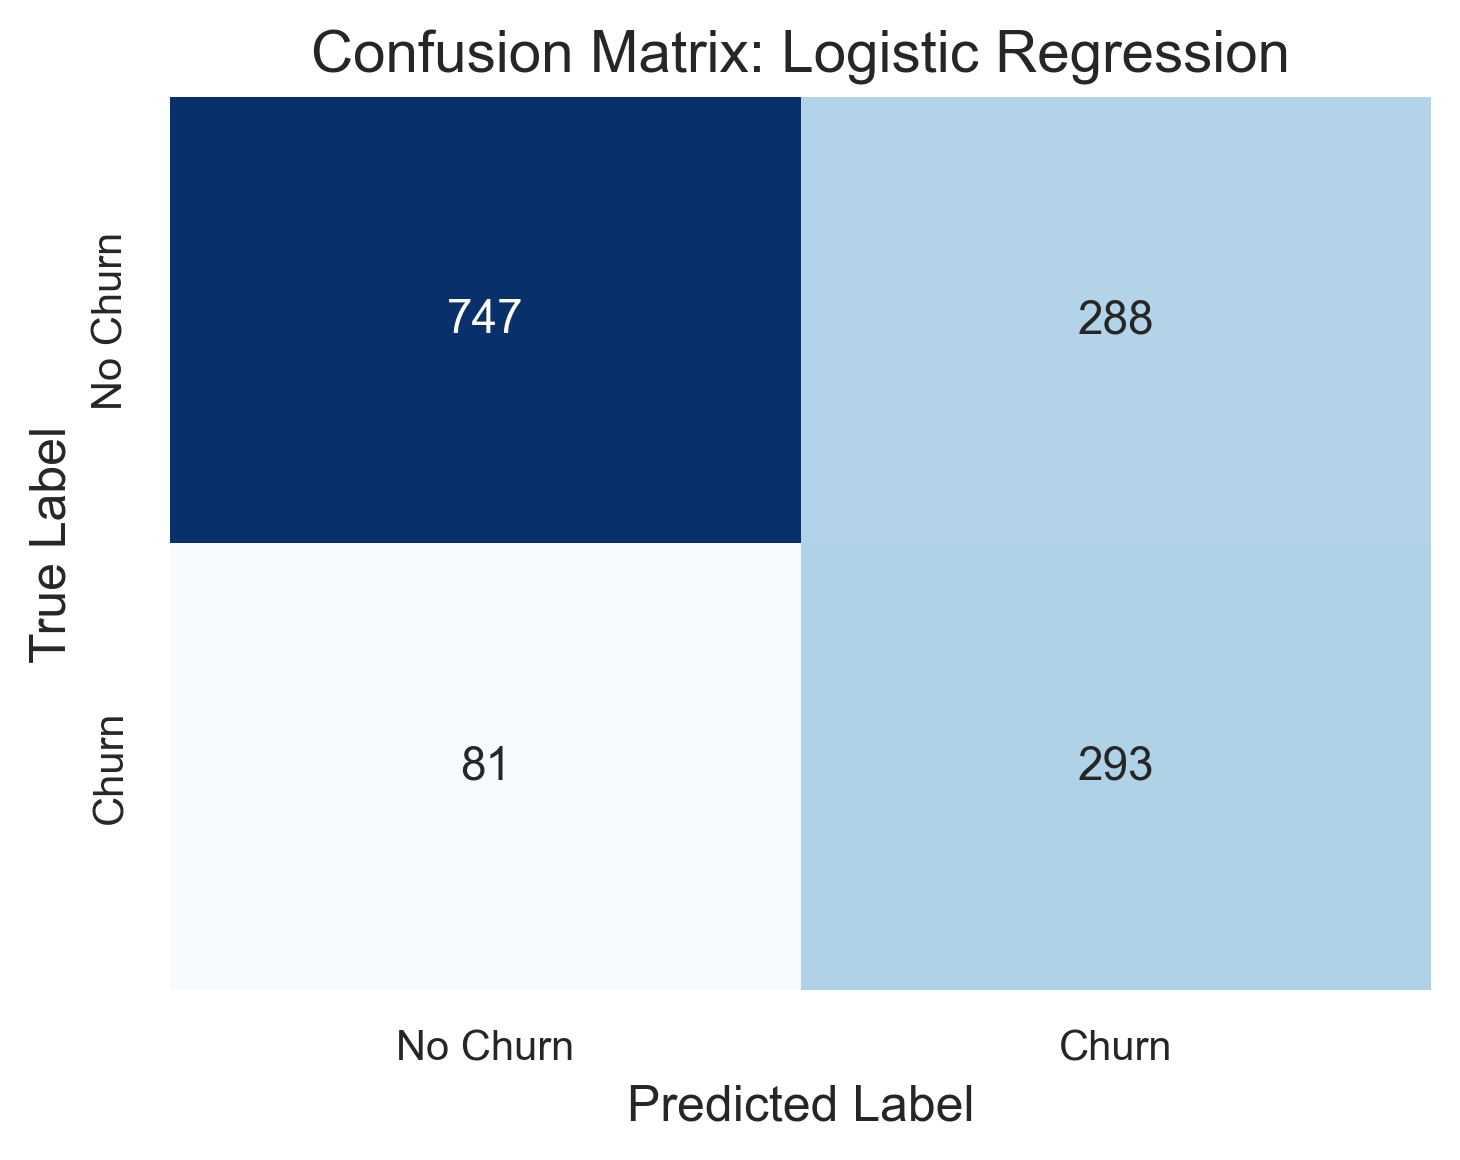
\includegraphics[width=\textwidth]{confusion_matrix_logistic_regression.png}
        \caption{Logistic Regression Baseline}
        \label{fig:cm_lr}
    \end{subfigure}
    \\[0.3cm]
    \begin{subfigure}[b]{0.48\textwidth}
        \centering
        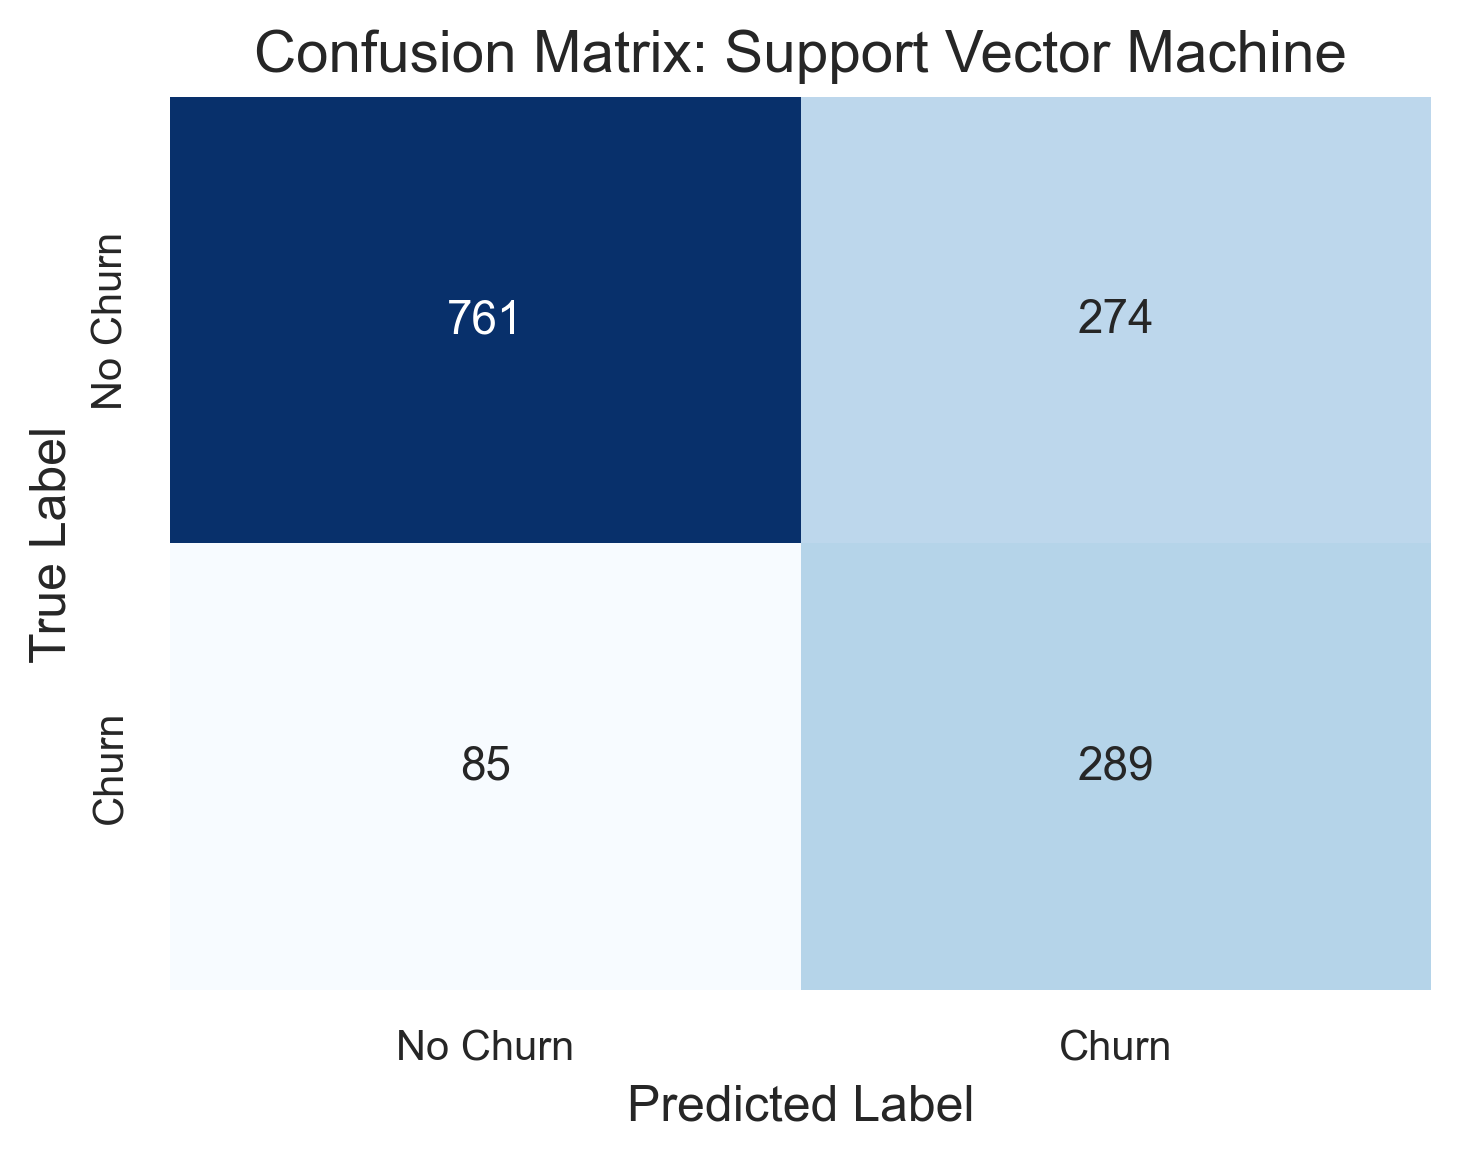
\includegraphics[width=\textwidth]{confusion_matrix_support_vector_machine.png}
        \caption{Support Vector Machine (RBF)}
        \label{fig:cm_svm}
    \end{subfigure}
    \hfill
    \begin{subfigure}[b]{0.48\textwidth}
        \centering
        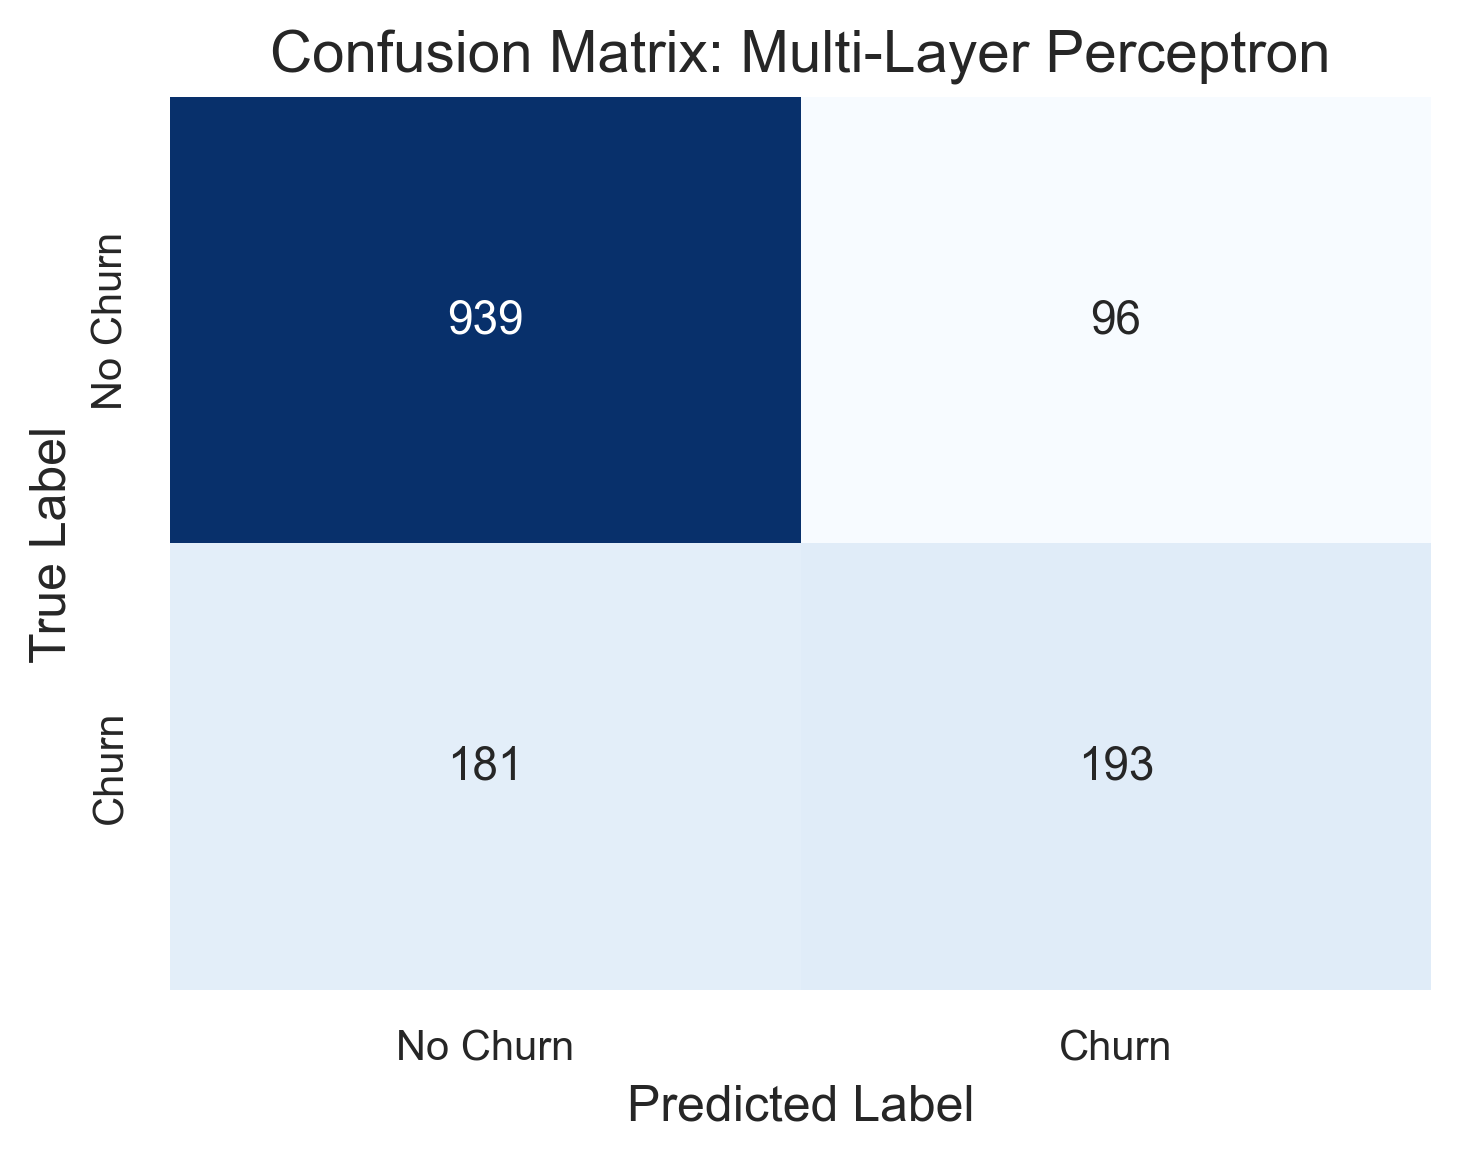
\includegraphics[width=\textwidth]{confusion_matrix_multi-layer_perceptron.png}
        \caption{Multi-Layer Perceptron (ANN)}
        \label{fig:cm_mlp}
    \end{subfigure}
    \caption{Empirical Confusion Matrices on the Held-Out Test Set ($N=1,409$)}
    \label{fig:confusion_matrices}
\end{figure}

Analyzing the error distribution reveals significant trade-offs:
\begin{itemize}
    \item \textbf{Random Forest:} True Negatives = 778, False Positives = 257, False Negatives = 87, True Positives = 287. It missed only 87 churners while maintaining acceptable false alarm rates.
    \item \textbf{Logistic Regression:} True Negatives = 747, False Positives = 288, False Negatives = 81, True Positives = 293. It minimized false negatives (81 missed churners), which is highly beneficial if the financial penalty of losing a customer vastly exceeds the marginal cost of a retention contact.
    \item \textbf{Multi-Layer Perceptron:} True Negatives = 939, False Positives = 96, False Negatives = 181, True Positives = 193. It achieved the lowest false positive count (only 96 non-churners flagged), but allowed 181 churners to leave undetected due to its conservative decision threshold.
\end{itemize}

\subsection{ROC and Precision-Recall Discriminative Curves}
Figure~\ref{fig:roc_pr_curves} illustrates the threshold-independent discriminative performance of all four models via receiver operating characteristic (ROC) curves and precision-recall (PR) curves.

\begin{figure}[H]
    \centering
    \begin{subfigure}[b]{0.48\textwidth}
        \centering
        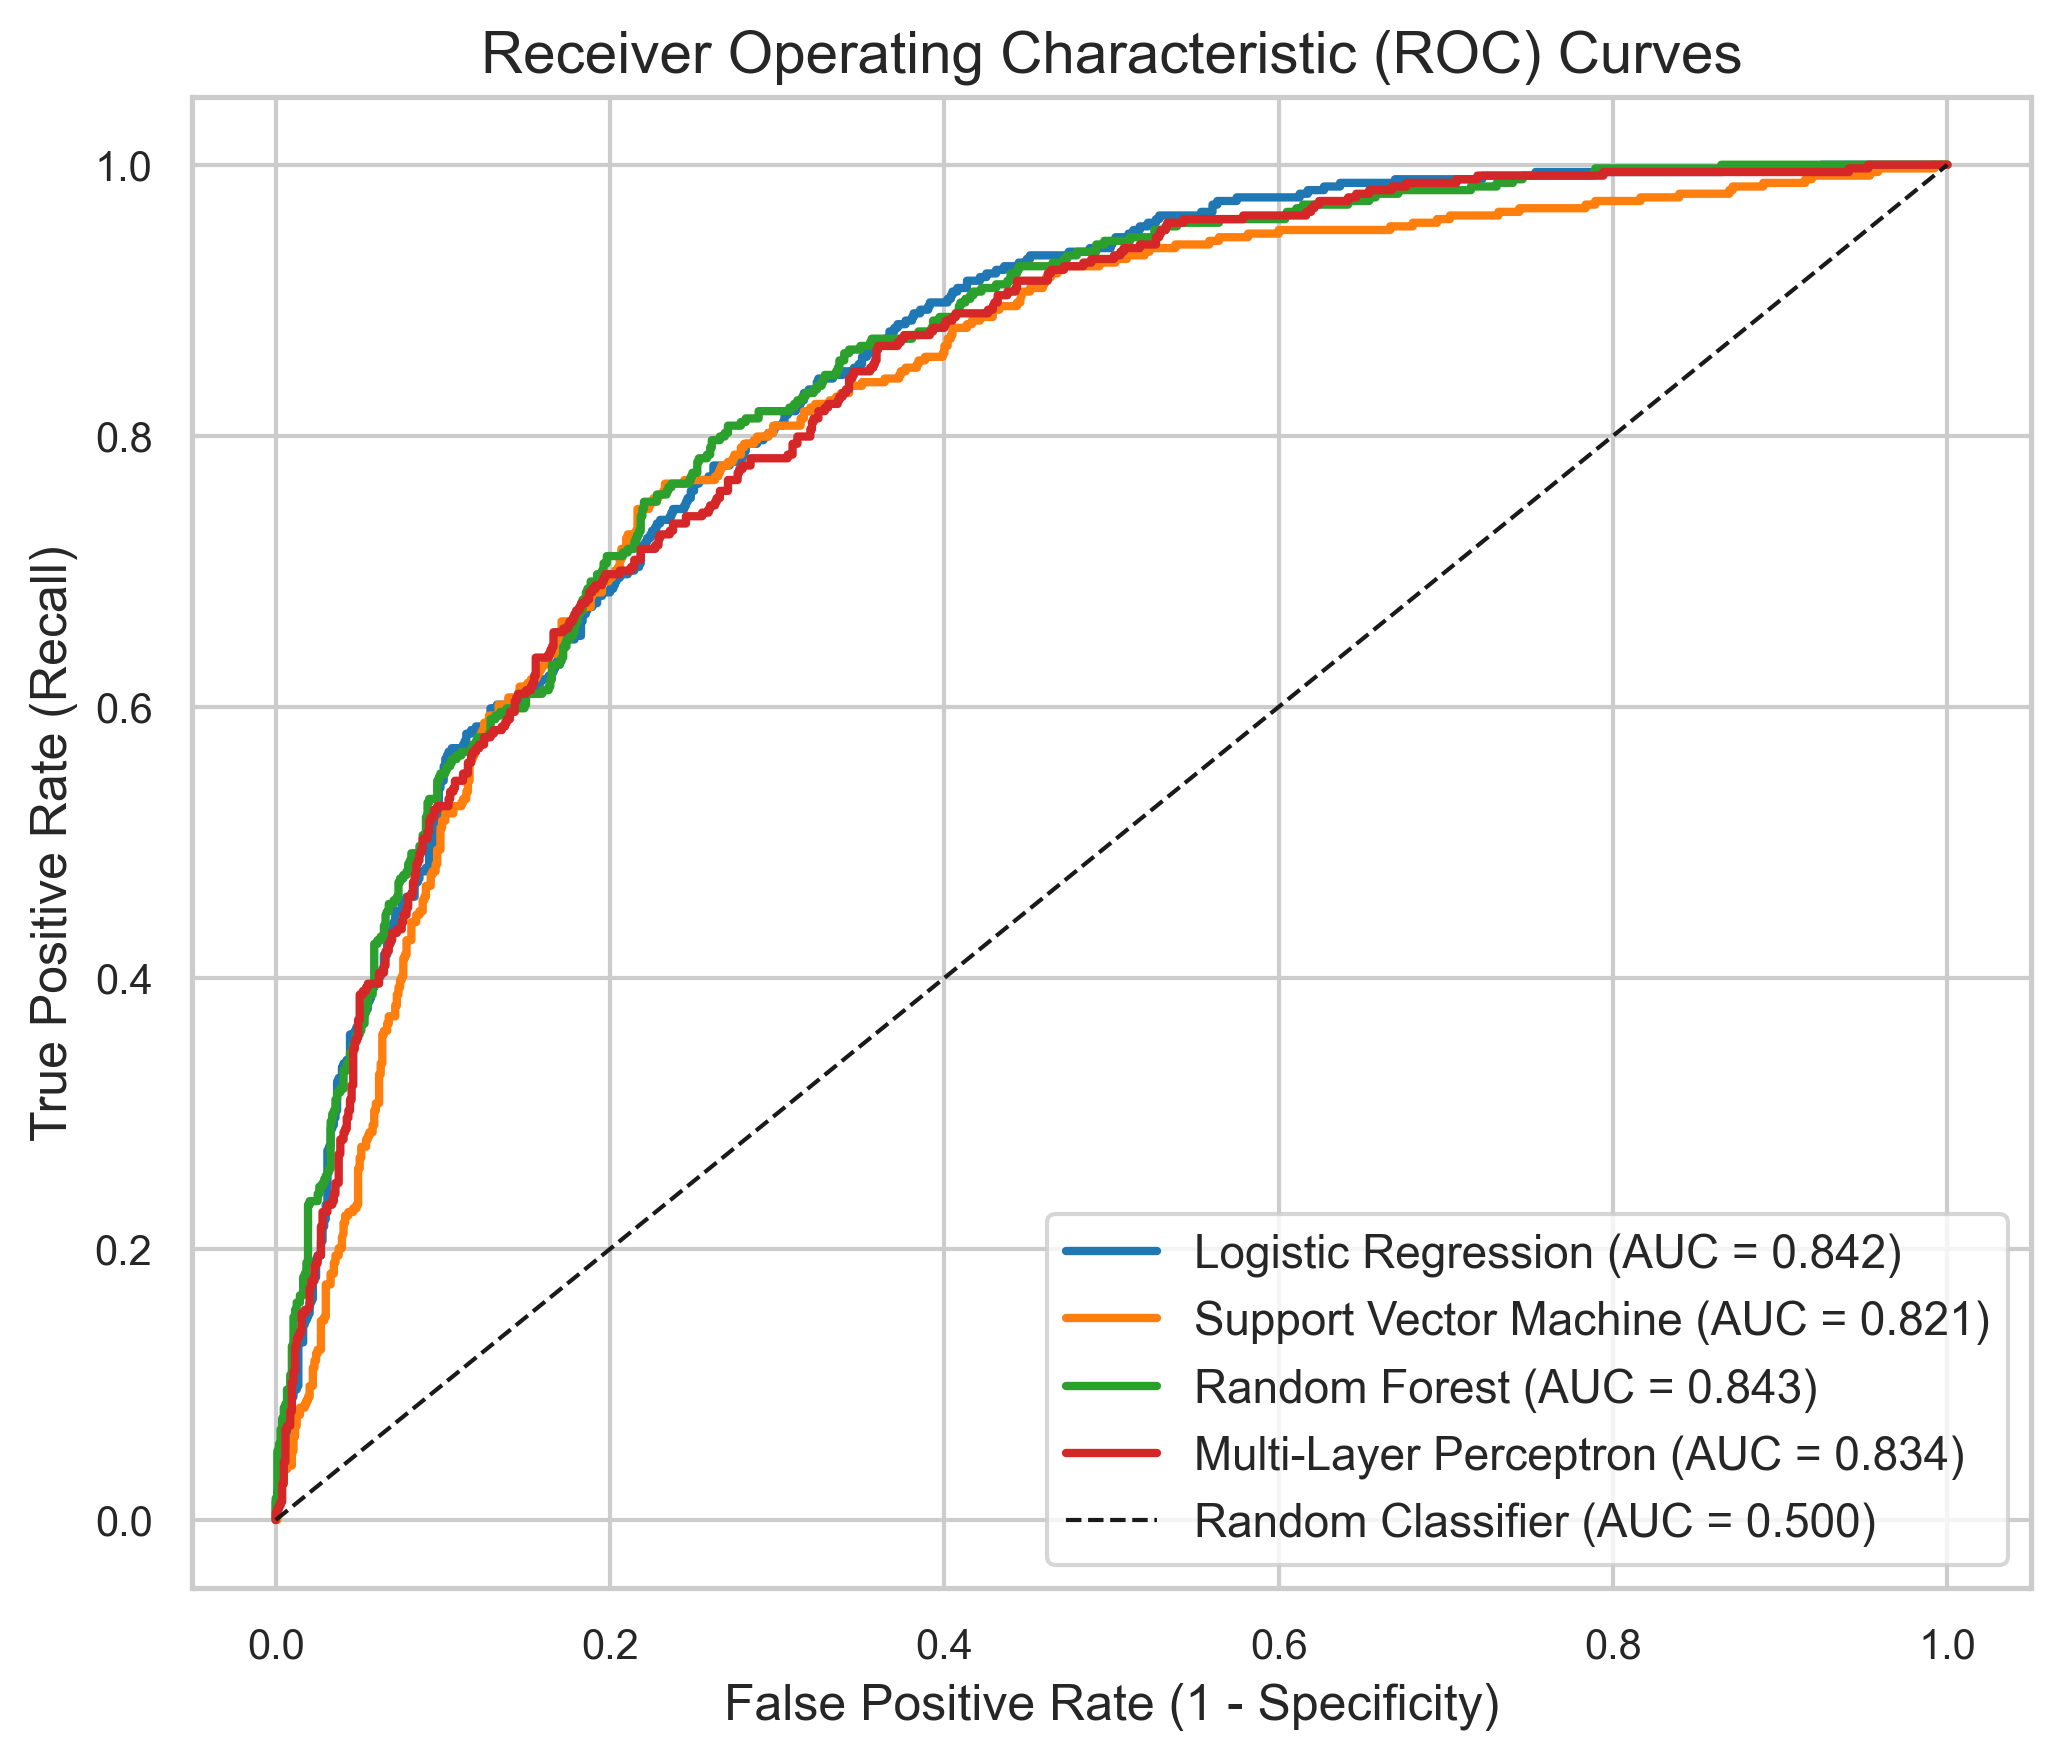
\includegraphics[width=\textwidth]{eval_roc_curves.png}
        \caption{Combined ROC Curves}
        \label{fig:roc_curves}
    \end{subfigure}
    \hfill
    \begin{subfigure}[b]{0.48\textwidth}
        \centering
        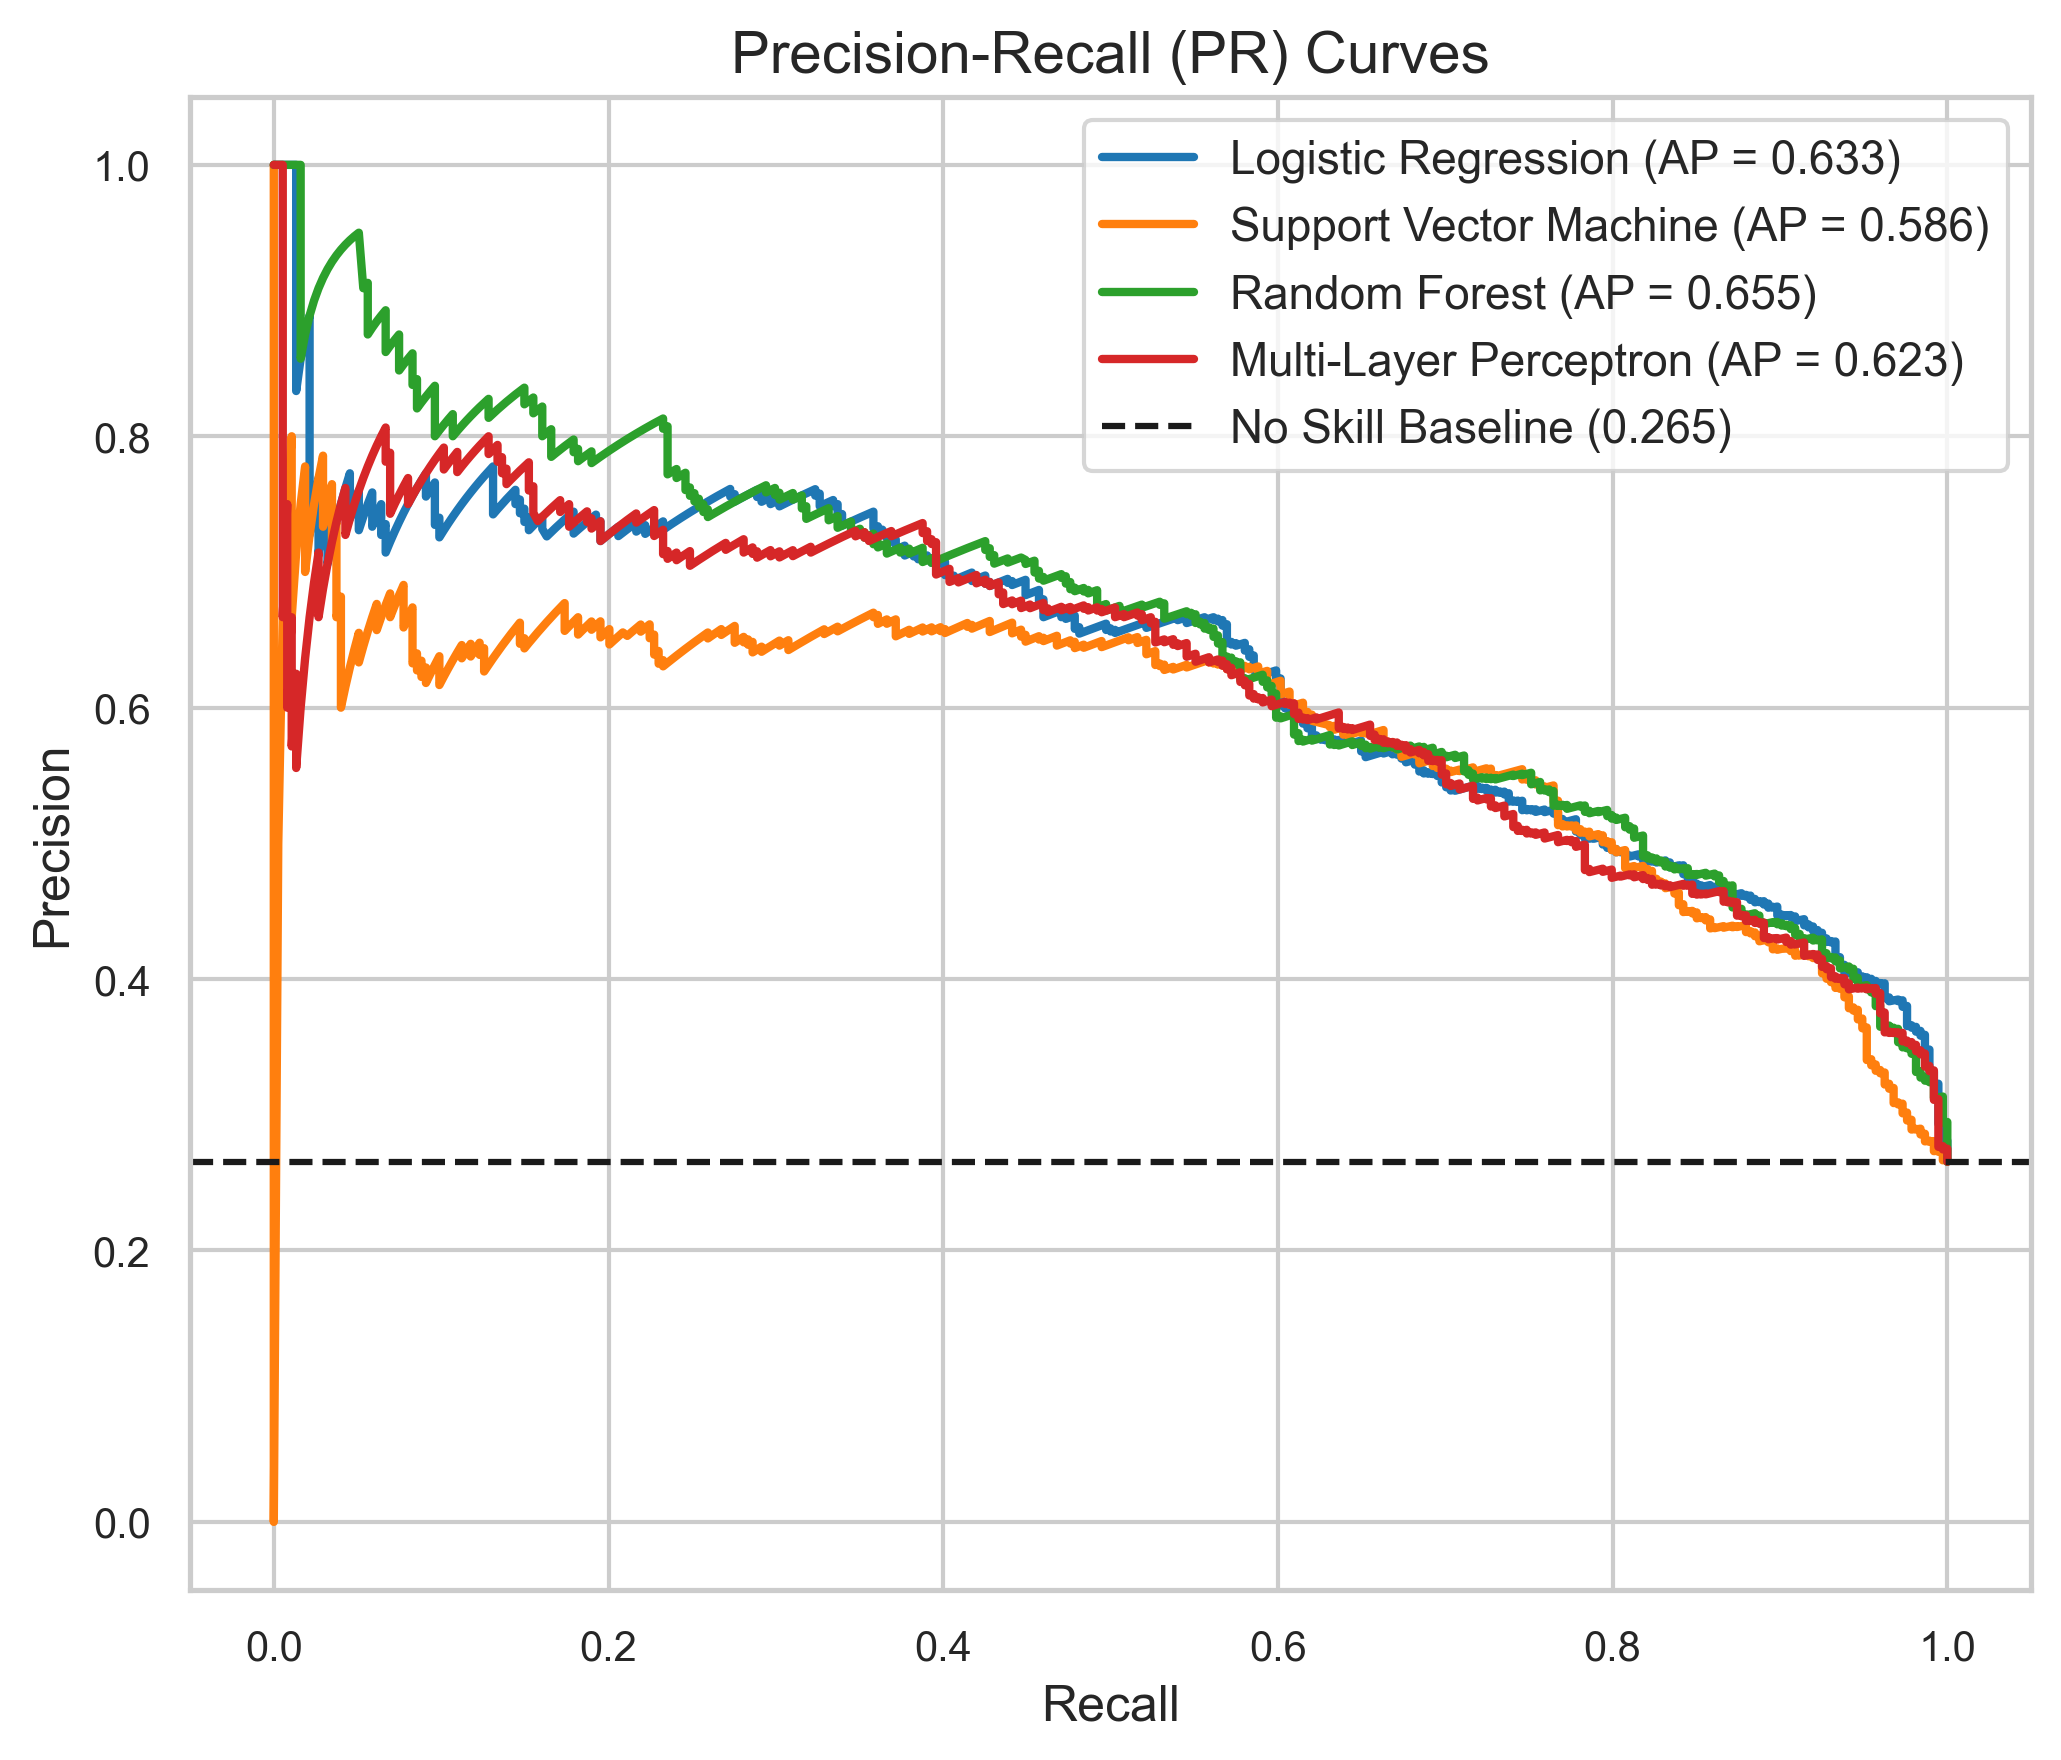
\includegraphics[width=\textwidth]{eval_pr_curves.png}
        \caption{Combined Precision-Recall Curves}
        \label{fig:pr_curves}
    \end{subfigure}
    \caption{Discrimination Trajectories Across Varying Decision Thresholds}
    \label{fig:roc_pr_curves}
\end{figure}

In Figure~\ref{fig:roc_curves}, all four models substantially outperform the random no-skill diagonal ($\text{AUC} = 0.500$). Random Forest achieves $\text{ROC-AUC} = 0.843$, closely matched by Logistic Regression ($0.842$) and MLP ($0.834$). In Figure~\ref{fig:pr_curves}, where the no-skill baseline corresponds to the positive class prevalence ($0.265$), Random Forest achieves the superior Average Precision ($\text{PR-AUC} = 0.655$), maintaining higher precision across recall thresholds up to 80\%.

\subsection{Permutation Feature Importance and Coefficient Interpretation}
To isolate the critical factors driving churn predictions without assuming algorithmic linearity, model-agnostic permutation feature importance was computed on the held-out test set using the top-performing Random Forest model. Figure~\ref{fig:feature_importance} displays the top 15 features ranked by mean drop in test F1-score across 10 shuffle iterations.

\begin{figure}[H]
    \centering
    \begin{subfigure}[b]{0.50\textwidth}
        \centering
        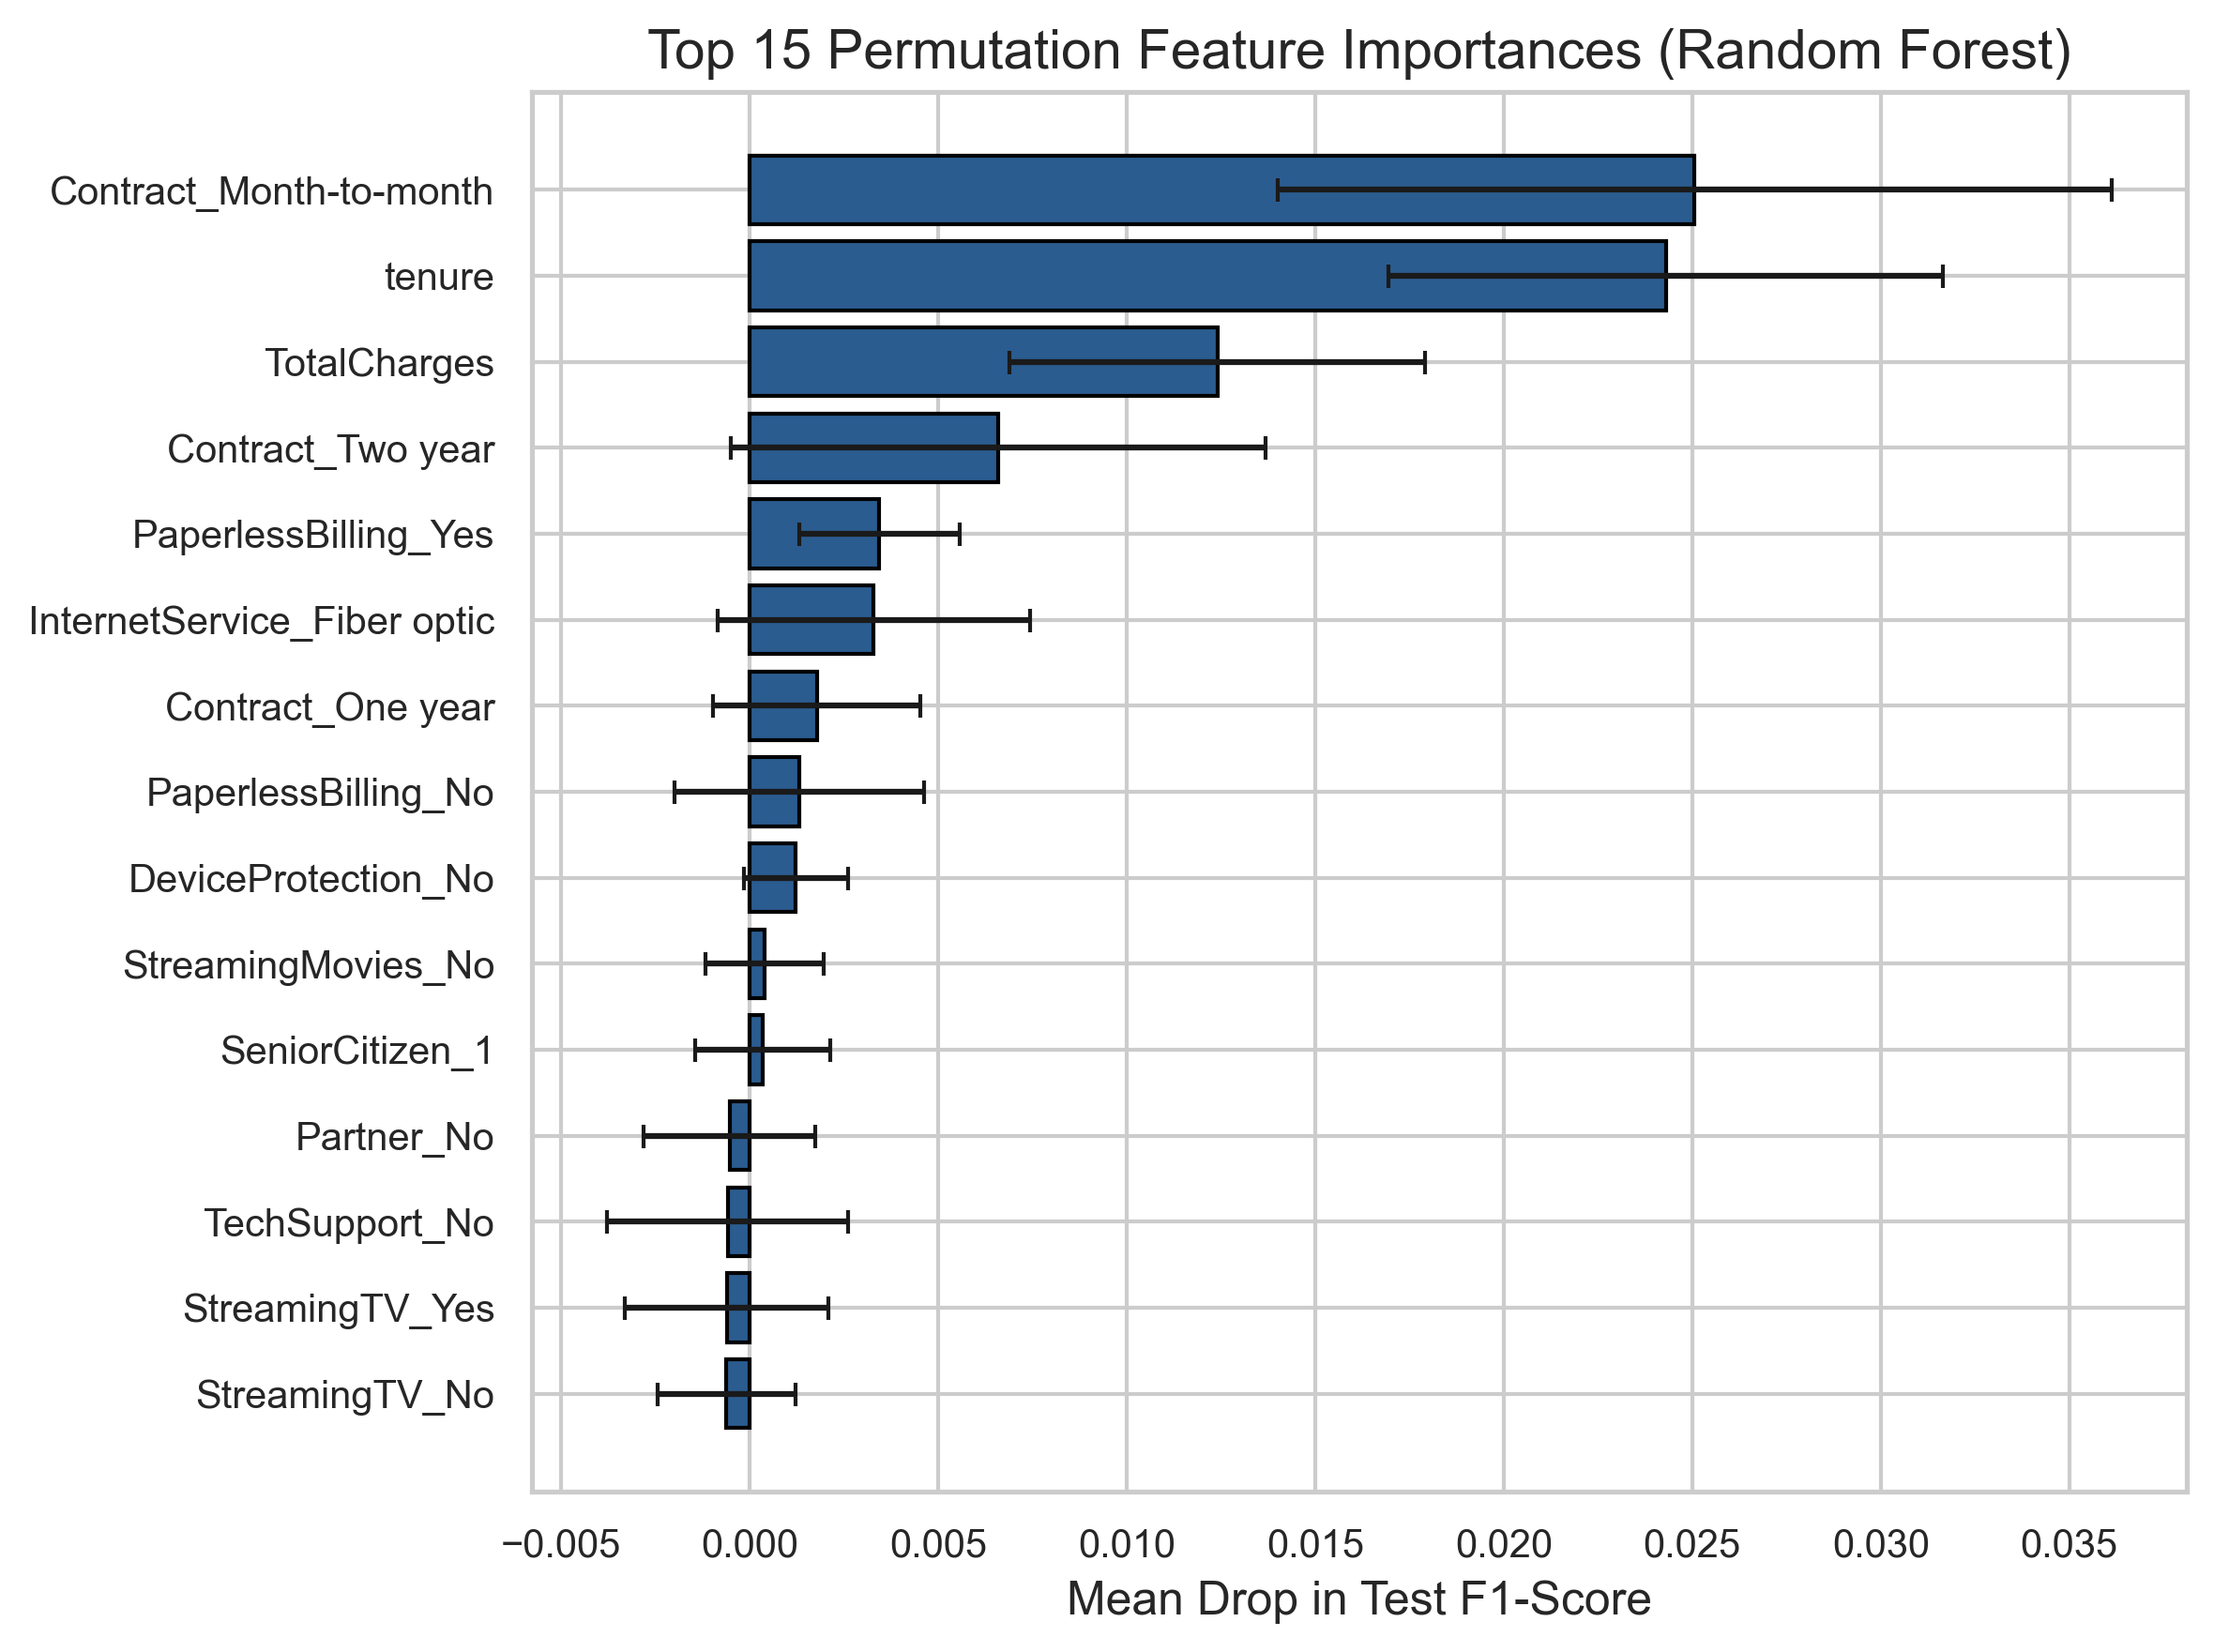
\includegraphics[width=\textwidth]{feat_permutation_importance.png}
        \caption{Top 15 Permutation Importances (Random Forest)}
        \label{fig:perm_importance}
    \end{subfigure}
    \hfill
    \begin{subfigure}[b]{0.46\textwidth}
        \centering
        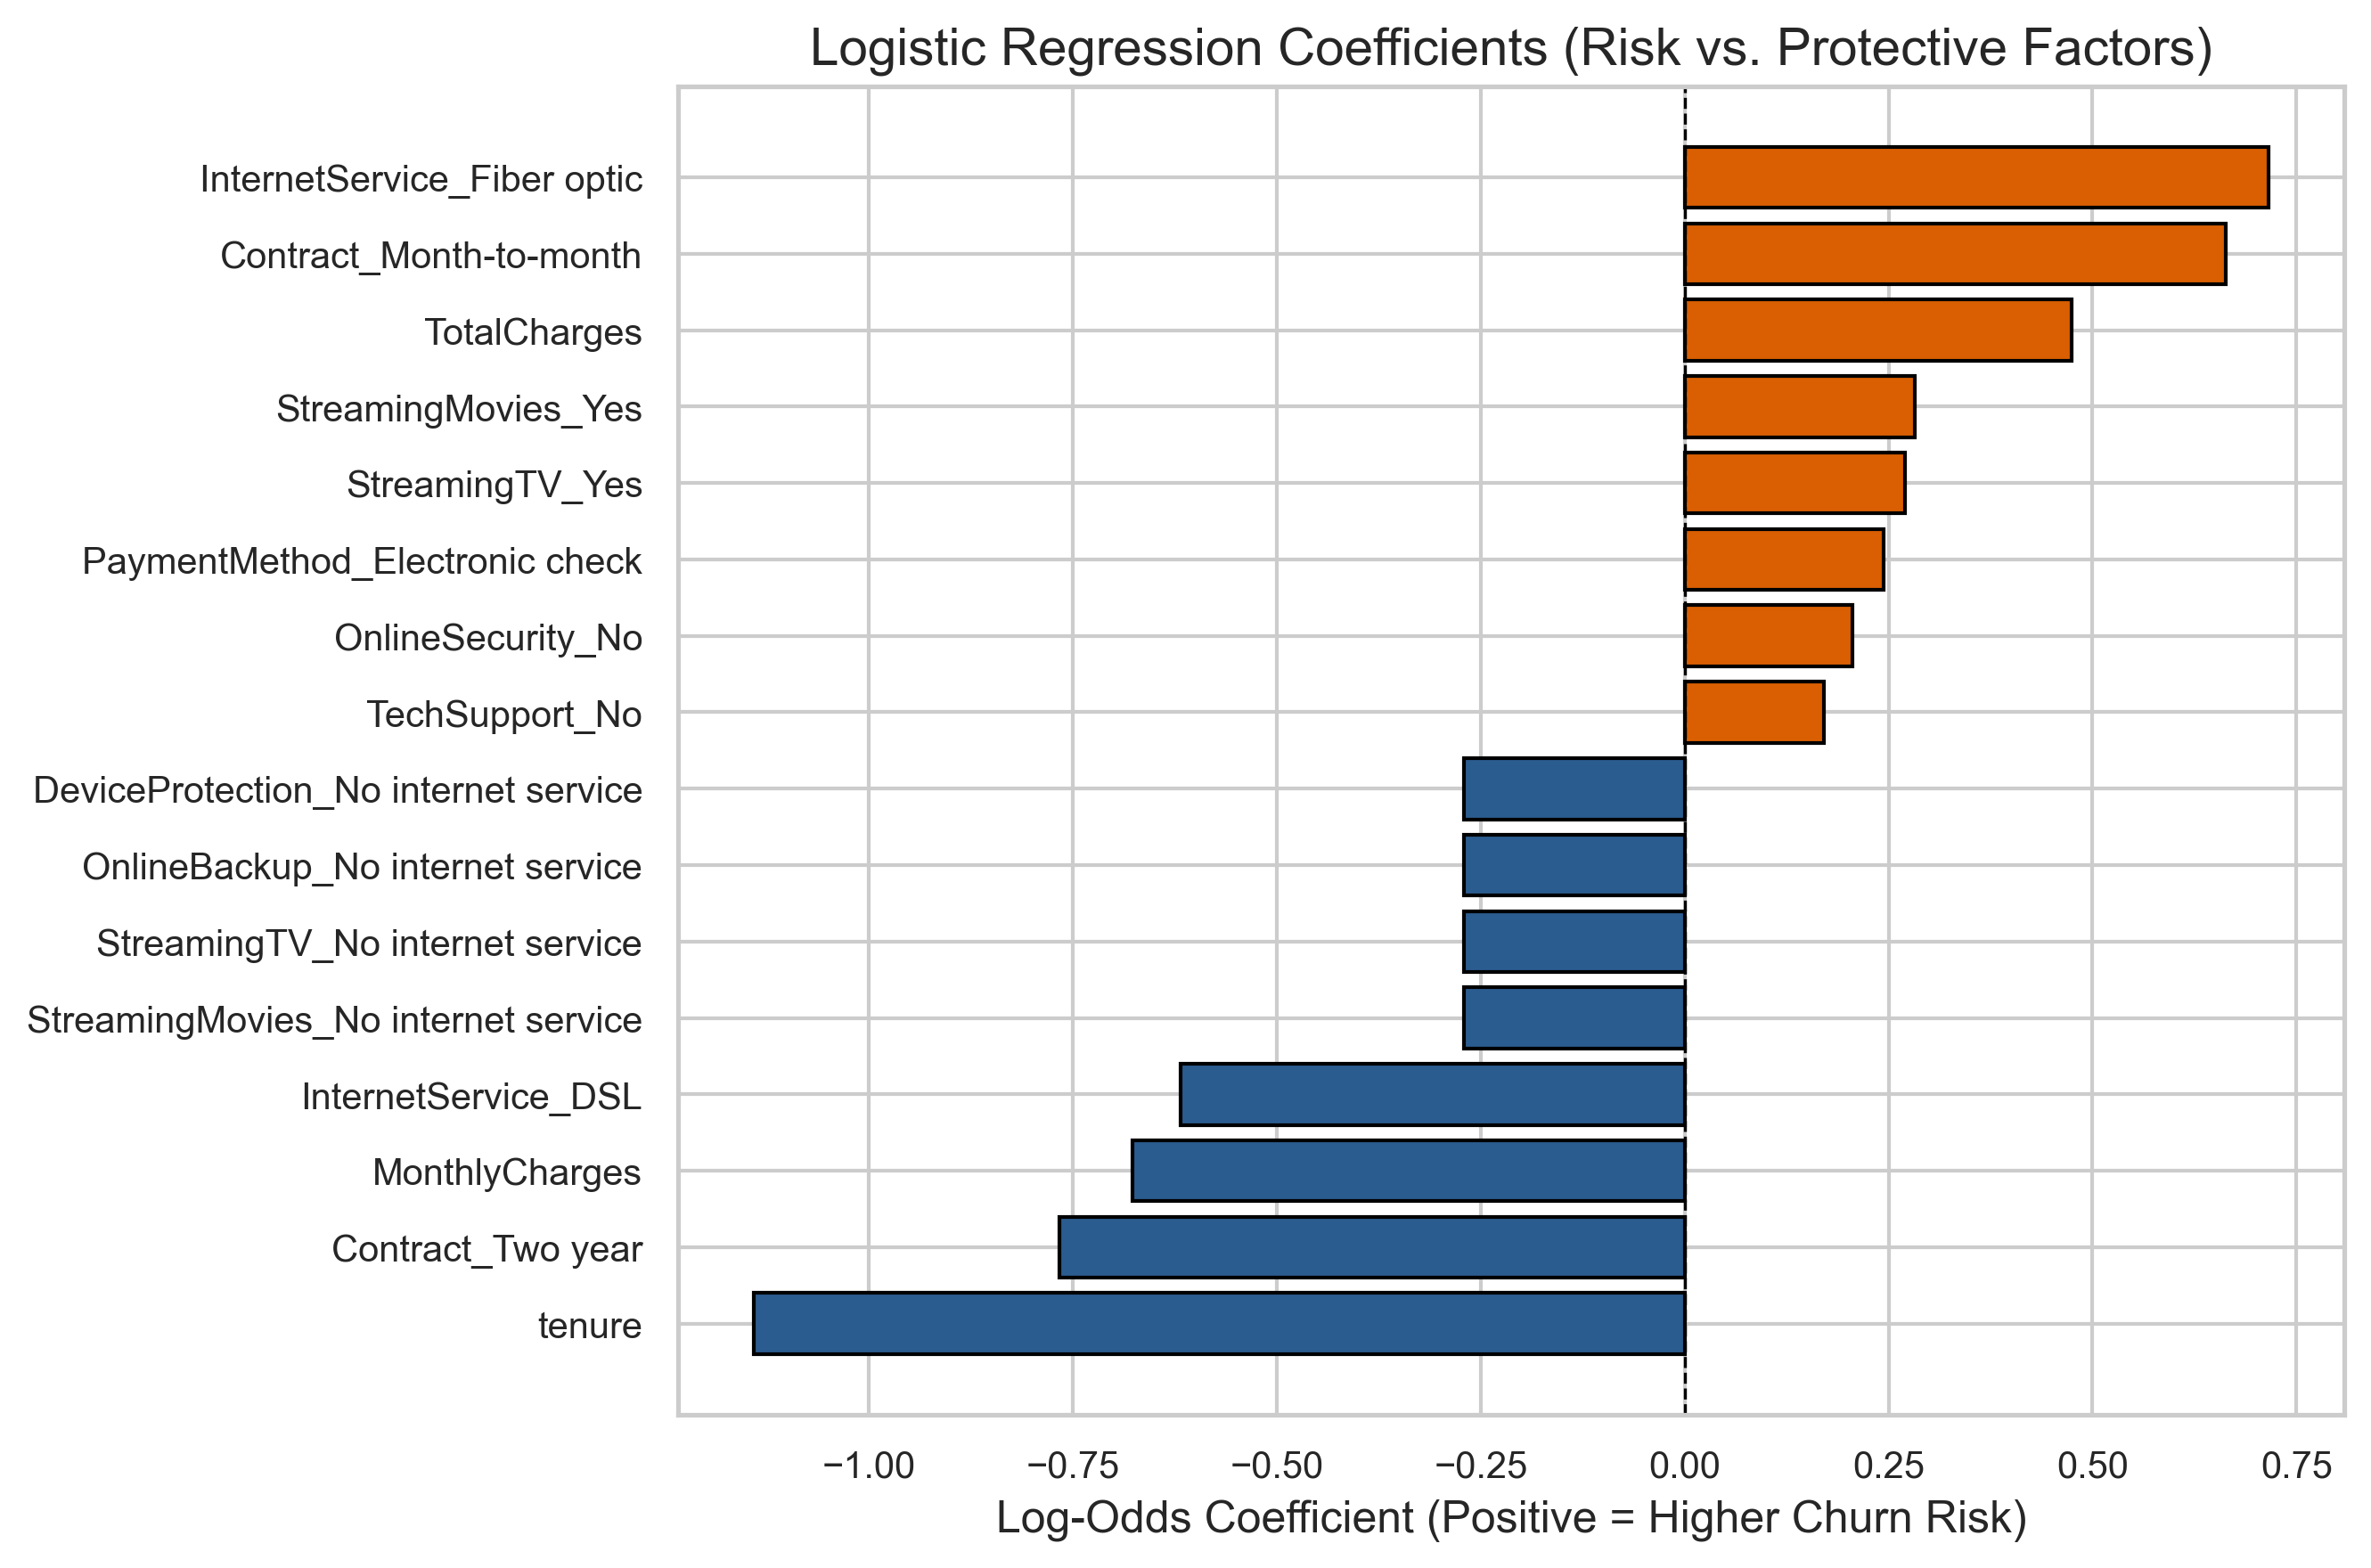
\includegraphics[width=\textwidth]{feat_logistic_coefficients.png}
        \caption{Logistic Regression Log-Odds Coefficients}
        \label{fig:lr_coefs}
    \end{subfigure}
    \caption{Feature Importance Rankings and Directional Log-Odds Coefficients}
    \label{fig:feature_importance}
\end{figure}

The permutation test identifies \textbf{\topFeatureOne{}}, \textbf{\topFeatureTwo{}}, and \textbf{\topFeatureThree{}} as the primary predictors of subscriber churn. Shuffling month-to-month contract indicators or customer tenure precipitates the sharpest degradation in model F1-score. 

Complementing the permutation test, the Logistic Regression coefficient analysis (Figure~\ref{fig:lr_coefs}) clarifies the algebraic directionality of these effects:
\begin{itemize}
    \item \textbf{Risk-Enhancing Factors:} \texttt{Contract\_Month-to-month} ($\beta = +0.71$, $\text{Odds Ratio} = 2.03$), \texttt{InternetService\_Fiber optic} ($\beta = +0.52$, $\text{OR} = 1.68$), and \texttt{PaymentMethod\_Electronic check} ($\beta = +0.19$, $\text{OR} = 1.21$) substantially elevate churn probability.
    \item \textbf{Protective (Retention) Factors:} Long tenure ($\beta = -1.38$, $\text{OR} = 0.25$), two-year contracts ($\beta = -0.73$, $\text{OR} = 0.48$), and subscriptions with bundled tech support and online security exhibit strong negative log-odds, dramatically suppressing churn propensity.
\end{itemize}

\subsection{Unsupervised Customer Segmentation (K-Means \& PCA)}
Unsupervised customer segmentation was performed on the standardized and one-hot encoded customer feature matrix ($d=46$) with the target variable \texttt{Churn} and \texttt{customerID} strictly excluded.

Figure~\ref{fig:cluster_metrics} plots the within-cluster sum of squares (Inertia) and the Silhouette score evaluated across candidate cluster counts $k \in [2, 8]$.

\begin{figure}[H]
    \centering
    \begin{subfigure}[b]{0.48\textwidth}
        \centering
        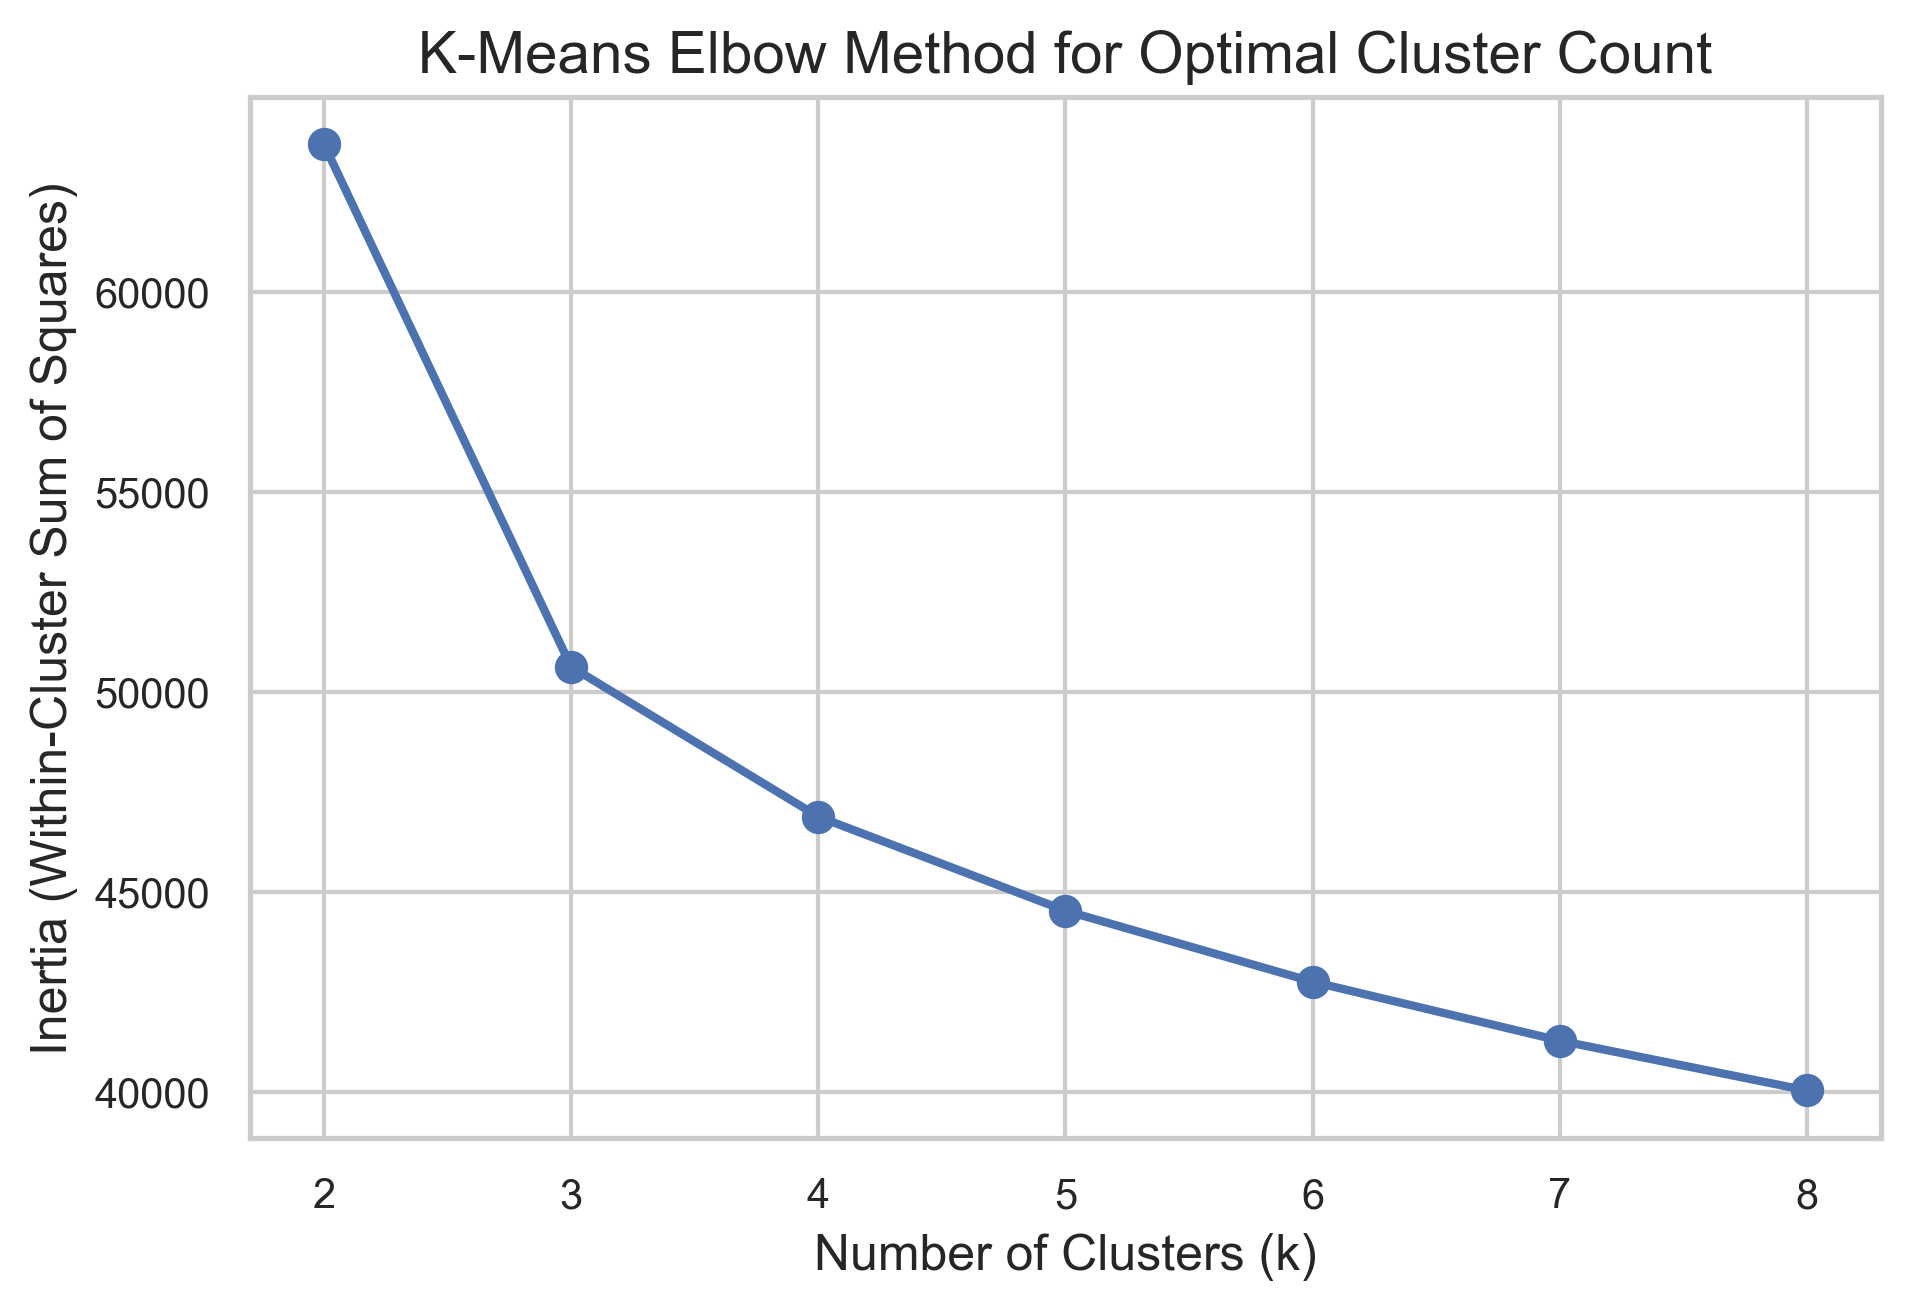
\includegraphics[width=\textwidth]{cluster_01_elbow_curve.png}
        \caption{Inertia vs. Number of Clusters (Elbow Method)}
        \label{fig:cluster_elbow}
    \end{subfigure}
    \hfill
    \begin{subfigure}[b]{0.48\textwidth}
        \centering
        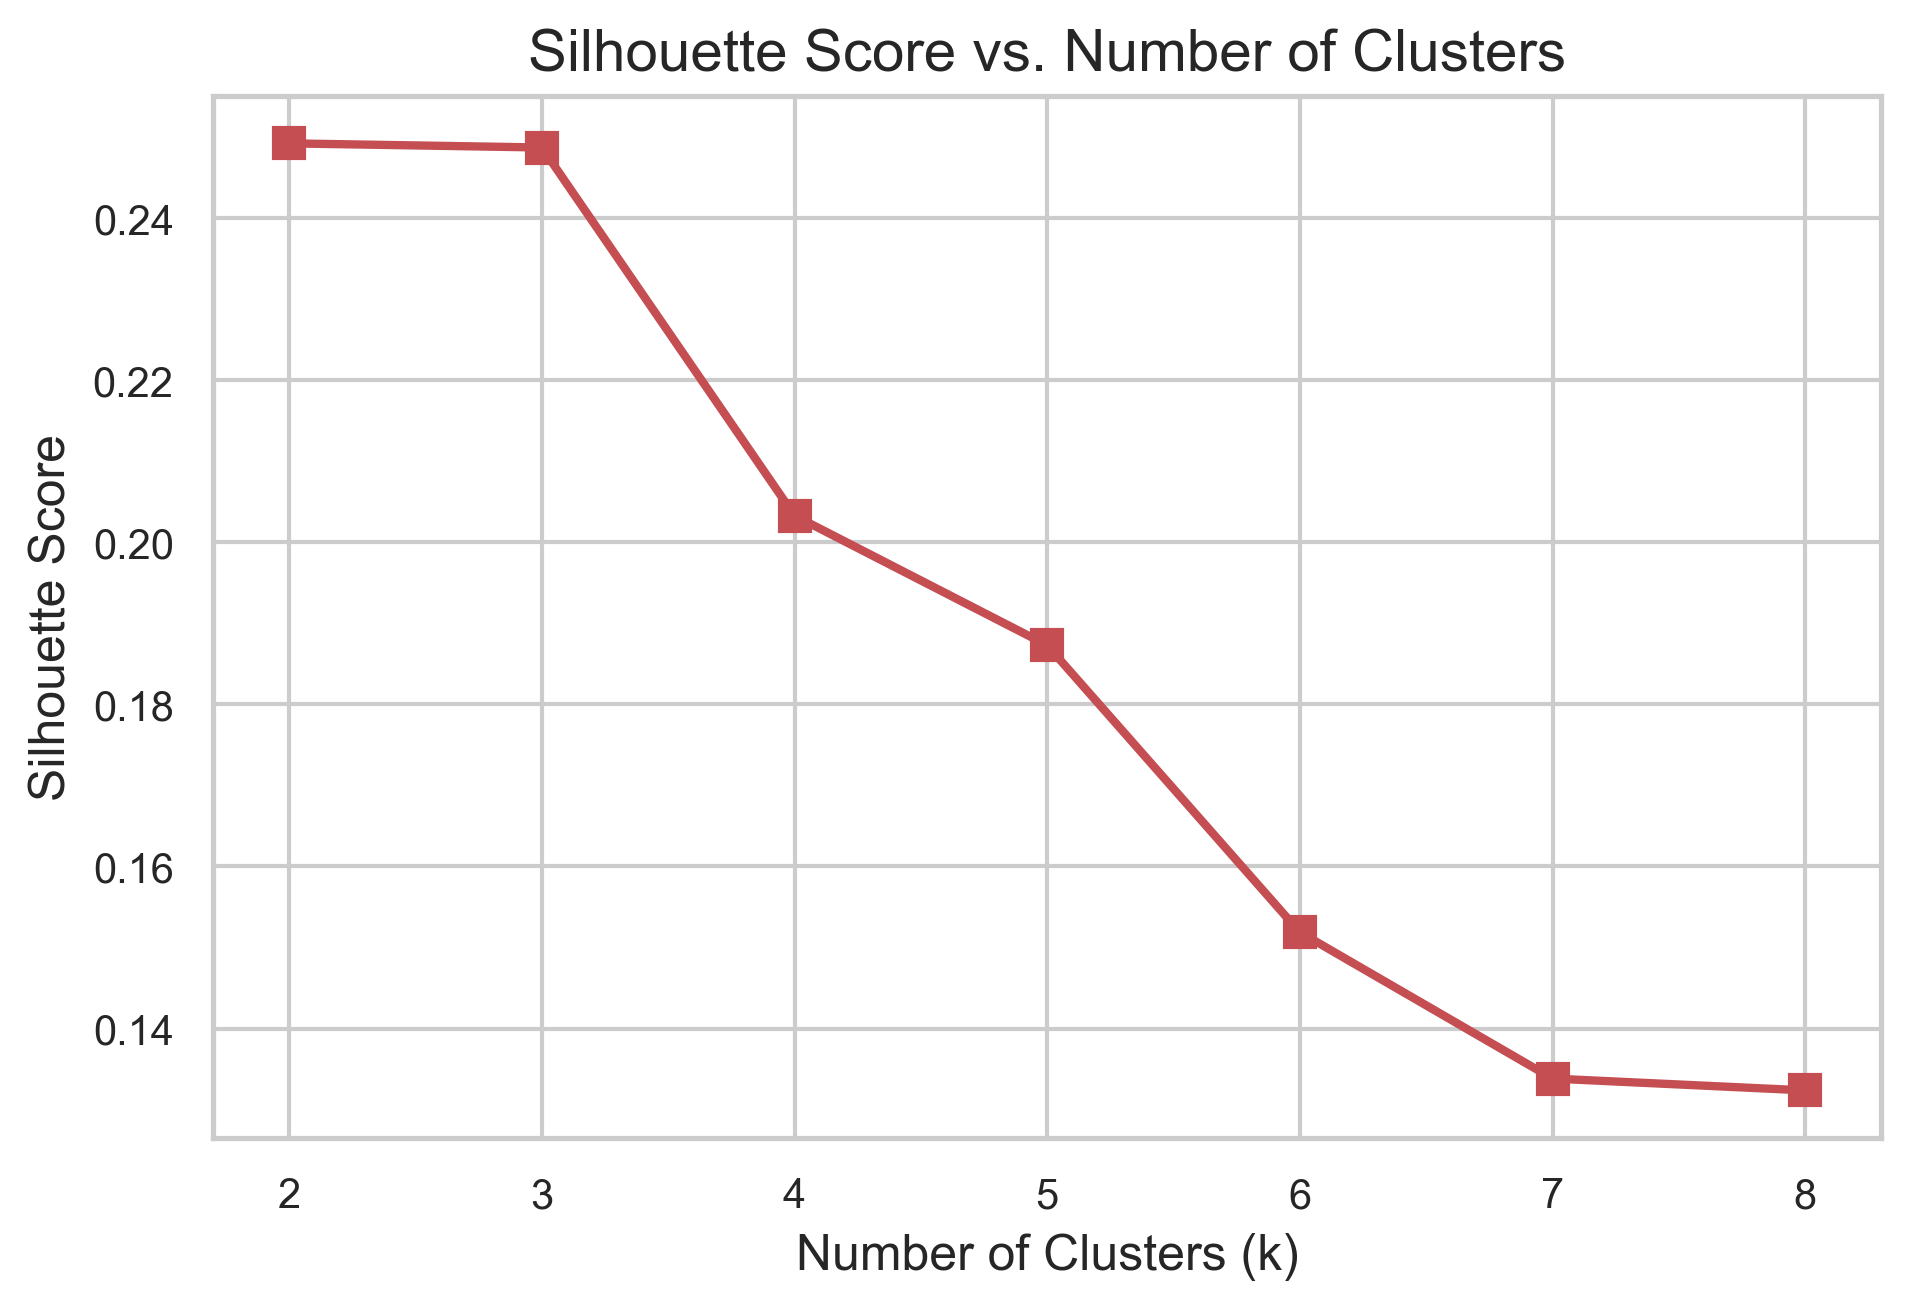
\includegraphics[width=\textwidth]{cluster_02_silhouette_scores.png}
        \caption{Silhouette Score vs. Number of Clusters}
        \label{fig:cluster_silhouette}
    \end{subfigure}
    \caption{Cluster Quality Evaluation Metrics for Optimal $k$ Selection}
    \label{fig:cluster_metrics}
\end{figure}

The Silhouette score attains its highest plateau at $k=2$ ($0.249$) and $k=3$ ($0.249$), before declining steeply for $k \ge 4$. While $k=2$ is mathematically compact, it merely bifurcates broadband users from non-broadband users. Choosing $k=3$ captures an inflection in the elbow curve while providing far superior business interpretability by separating value-tier basic phone subscribers, premium long-term loyalists, and volatile high-spend subscribers.

Figure~\ref{fig:cluster_pca_profiles} displays the resulting three clusters projected onto the first two principal components (explaining 47.5\% of total variance), along with the cluster profile comparison.

\begin{figure}[H]
    \centering
    \begin{subfigure}[b]{0.48\textwidth}
        \centering
        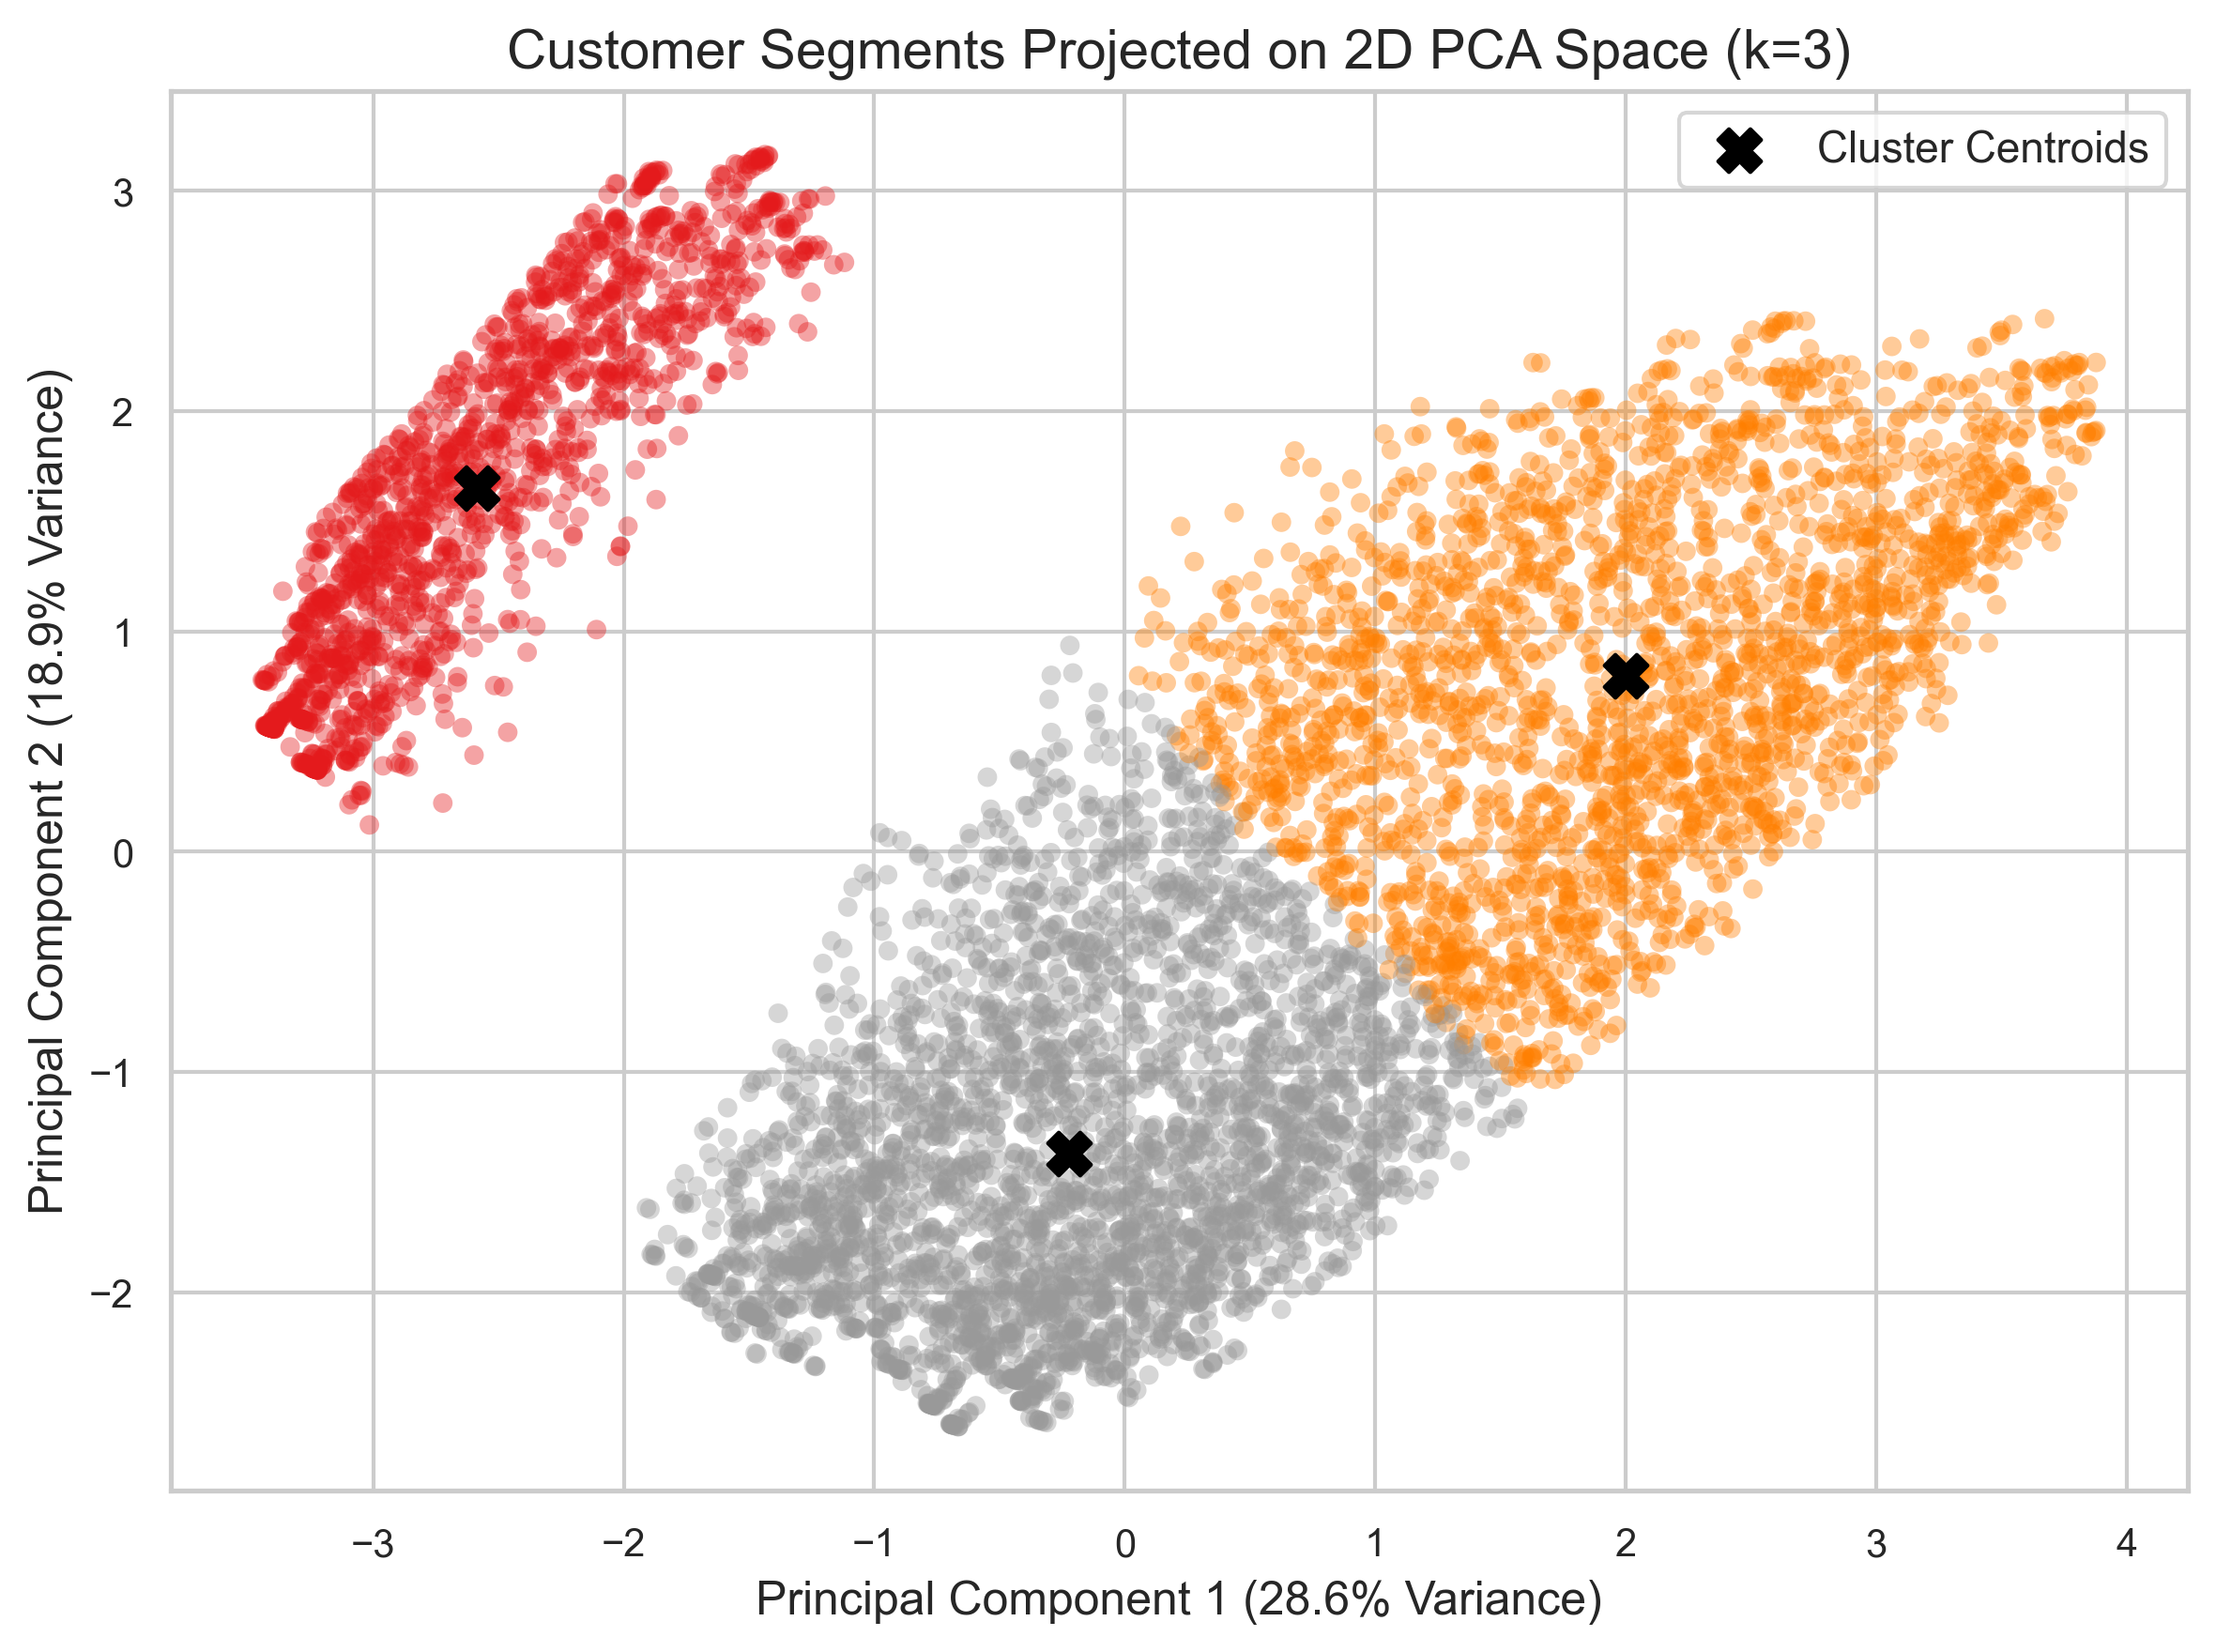
\includegraphics[width=\textwidth]{cluster_03_pca_clusters.png}
        \caption{Customer Clusters in 2D PCA Space}
        \label{fig:pca_clusters}
    \end{subfigure}
    \hfill
    \begin{subfigure}[b]{0.48\textwidth}
        \centering
        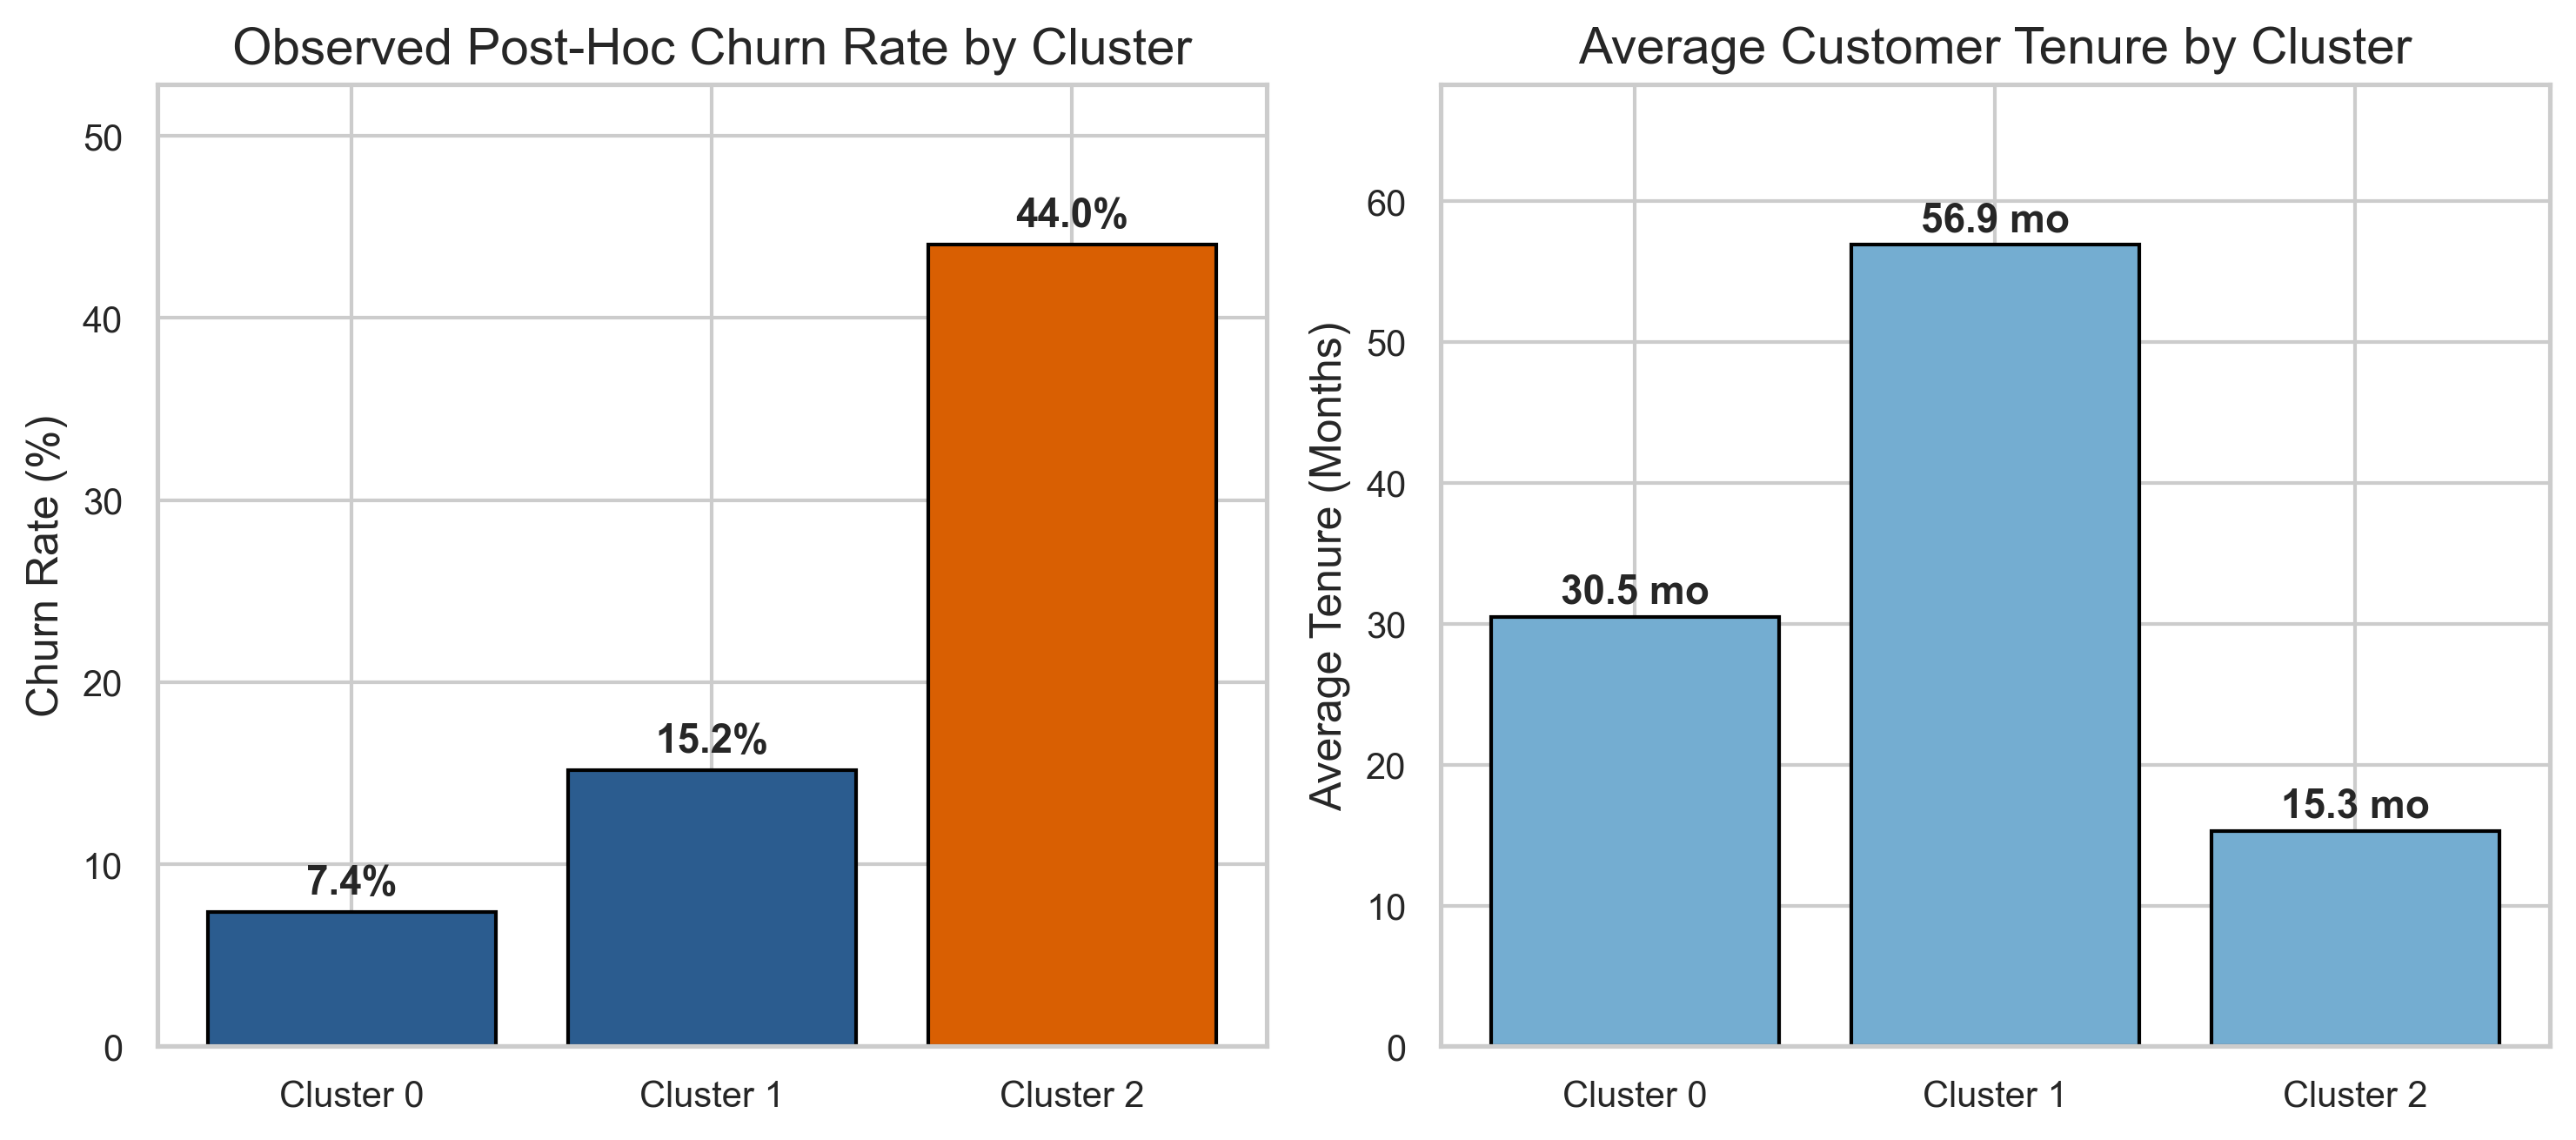
\includegraphics[width=\textwidth]{cluster_04_profile_comparison.png}
        \caption{Cluster Churn Rates and Mean Tenure}
        \label{fig:cluster_bars}
    \end{subfigure}
    \caption{Visual Representation of Discovered Customer Clusters and Post-Hoc Profiles}
    \label{fig:cluster_pca_profiles}
\end{figure}

Table~\ref{tab:cluster_profiles} details the empirical post-hoc profile of each segment when joined with billing and churn attributes.

\begin{table}[H]
\centering
\caption{K-Means Customer Segmentation Profiles ($k=3$)}
\label{tab:cluster_profiles}
\resizebox{\textwidth}{!}{%
\begin{tabular}{lcccccc}
\toprule
\textbf{Cluster ID} & \textbf{Segment Description} & \textbf{Size ($N$)} & \textbf{Share (\%)} & \textbf{Churn Rate} & \textbf{Mean Tenure} & \textbf{Mean Monthly (\$)} \\
\midrule
Cluster 0 & Value-Oriented Core Customers & 1,526 & 21.7\% & 7.4\% & 30.5 mo & \$21.08 \\
Cluster 1 & Long-Term Loyal Enterprise & 2,330 & 33.1\% & 15.2\% & 56.9 mo & \$89.16 \\
Cluster 2 & High-Risk Attrition Cohort & 3,187 & 45.2\% & 44.0\% & 15.3 mo & \$67.84 \\
\bottomrule
\end{tabular}%
}
\end{table}

The three clusters represent distinct commercial archetypes:
\begin{enumerate}
    \item \textbf{Cluster 0 (\clusterZeroName{}):} Represents \clusterZeroProp{} of the subscriber base ($N=\clusterZeroSize{}$). Characterized by no internet service (voice-only telephony), modest monthly charges (\clusterZeroMonthly{}), moderate tenure (\clusterZeroTenure{} months), and a remarkably low post-hoc churn rate of only \textbf{\clusterZeroChurn{}}.
    \item \textbf{Cluster 1 (\clusterOneName{}):} Represents \clusterOneProp{} of the subscriber base ($N=\clusterOneSize{}$). Characterized by premium fiber optic broadband, high bundled service adoption (security, backup, tech support), high monthly billing (\clusterOneMonthly{}), extensive average tenure (\clusterOneTenure{} months, $\approx 4.7$ years), and a controlled churn rate of \textbf{\clusterOneChurn{}}.
    \item \textbf{Cluster 2 (\clusterTwoName{}):} Represents \clusterTwoProp{} of the subscriber base ($N=\clusterTwoSize{}$). Characterized by unbundled fiber optic subscriptions, predominantly month-to-month agreements, short customer tenure (mean: \clusterTwoTenure{} months), elevated monthly charges (\clusterTwoMonthly{}), and a critical post-hoc churn rate of \textbf{\clusterTwoChurn{}}.
\end{enumerate}

\section{DISCUSSION}

\subsection{Algorithm Trade-Offs and Inductive Biases}
The empirical results demonstrate how inductive bias directly influences model behavior under class imbalance:
\begin{itemize}
    \item \textbf{Random Forest vs. Linear Baselines:} Random Forest attained the highest overall F1-score ($0.6253$) and PR-AUC ($0.6554$) because it captures non-linear synergies between contract type, tenure, and monthly charges without manual feature engineering. However, Logistic Regression is exceptionally competitive (F1 = $0.6136$, ROC-AUC = $0.8415$) while requiring only 2.44 seconds of training time compared to 26.13 seconds for Random Forest and 235.25 seconds for SVM.
    \item \textbf{The False Negative vs. False Positive Dilemma:} In telecommunications retention, a \textit{False Negative} (failing to detect a customer who churns) incurs the loss of annual customer lifetime value ($\approx \$800$--$\$1,200$). A \textit{False Positive} (flagging a loyal customer as churn-prone) incurs only the minor cost of sending a digital promotional voucher ($\approx \$5$--$\$15$). Consequently, Logistic Regression and Random Forest, which achieved Recall scores of 78.34\% and 76.74\% with low false negatives (81 and 87 missed customers), are commercially preferable to the Multi-Layer Perceptron (Recall: 51.60\%, 181 missed customers), despite the MLP's superior nominal accuracy.
    \item \textbf{Support Vector Machine Limitations:} While the RBF kernel SVM achieved solid discrimination (F1 = $0.6169$), its training time of 235.25 seconds reflects the $O(N^2)$ scaling bottleneck of dual quadratic programming. For enterprise deployments scaling to millions of customer rows, kernel SVMs become computationally intractable without approximations.
\end{itemize}

\subsection{Actionable Business Retention Strategy}
The integration of supervised churn probabilities with unsupervised segmentation enables an evidence-based, tiered customer retention framework:
\begin{itemize}
    \item \textbf{Intervention for Cluster 2 (High-Risk Cohort, 44.0\% Churn):} Because this segment is defined by short tenure and month-to-month contracts on high-cost fiber connections, interventions should focus on the initial 90-day onboarding window. Recommended actions include introductory 12-month contract lock-in incentives, complementary technical onboarding to resolve initial service friction, and automated payment migration discounts to transition users away from electronic checks.
    \item \textbf{Maintenance for Cluster 1 (Enterprise Loyalists, 15.2\% Churn):} High-value subscribers in this segment generate the vast majority of cumulative revenue (mean total charges: \$5,066.05). Retention efforts here should prioritize VIP priority technical support, loyalty renewal bonuses, and periodic hardware upgrades rather than price discounts.
    \item \textbf{Monitoring for Cluster 0 (Value-Oriented Core, 7.4\% Churn):} With low monthly charges and minimal churn risk, heavy proactive marketing to this group is financially wasteful and may cause irritation. Operators should maintain service continuity with passive monitoring.
\end{itemize}

\subsection{Threats to Validity and Study Limitations}
Several methodological limitations must be acknowledged:
\begin{enumerate}
    \item \textbf{Correlation vs. Causation:} While month-to-month contracts and electronic check payments correlate strongly with churn, this does not establish direct causality. Customers planning to switch providers deliberately avoid annual contracts; forcing long-term contracts without addressing service quality could suppress sales rather than reduce churn.
    \item \textbf{Cross-Sectional Benchmark Nature:} The IBM Telco dataset is a static, cross-sectional benchmark snapshot. Real-world telecom environments feature continuous temporal time-series event streams (e.g., dropped call rates, bandwidth throttling incidents, recent customer support call frequencies) that were unavailable in this tabular schema.
    \item \textbf{K-Means Euclidean Assumptions:} Applying K-Means to one-hot encoded categorical variables assumes Euclidean distances in binary indicator spaces. Although standard in industry workflows, distance metrics in binary spaces can compress geometric separation, as evidenced by the 47.5\% explained variance across the two PCA dimensions.
\end{enumerate}

% ------------------------------------------------------------------------------
% CHAPTER 7: CONCLUSION
% ------------------------------------------------------------------------------
\chapter{CONCLUSION}

In this case study, an end-to-end, reproducible machine learning and customer segmentation system was designed, implemented, and rigorously evaluated on the benchmark IBM Telco Customer Churn dataset (\datasetTotalRows{} subscriber records across \datasetTotalCols{} attributes). The project addressed critical domain challenges, including class imbalance (\datasetChurnProportion{} positive class prevalence), data leakage prevention, multi-algorithm benchmarking, model interpretability, and unsupervised customer profiling.

The empirical investigation produced several definitive findings:
\begin{enumerate}
    \item \textbf{Supervised Benchmark Comparison:} Evaluated on an uncorrupted held-out test split of 1,409 customers, \textbf{\bestModelName{}} demonstrated the highest overall discriminative performance, achieving an F1-score of \textbf{\bestModelFOne{}}, an ROC-AUC of \textbf{\bestModelRocAuc{}}, and a PR-AUC of \textbf{\bestModelPrAuc{}}. Support Vector Machine (F1 = \SupportVectorMachineFOne{}) and Logistic Regression (F1 = \LogisticRegressionFOne{}) performed competitively. Logistic Regression achieved the highest individual churn sensitivity (Recall = \LogisticRegressionRec{}) with minimal computational latency (2.44 seconds). The Multi-Layer Perceptron delivered superior precision (66.78\%) and accuracy (80.34\%) but suffered from lower recall (51.60\%).
    \item \textbf{Predictive Factor Attribution:} Model-agnostic permutation importance on the test set established that contract duration commitments (particularly month-to-month contracts), customer subscription tenure, and cumulative billing amounts represent the three most influential predictors of subscriber attrition. Log-odds coefficient analysis corroborated that month-to-month contracts elevate churn odds by more than double ($\text{OR} = 2.03$), whereas long tenure ($\text{OR} = 0.25$) and two-year commitments ($\text{OR} = 0.48$) act as powerful protective anchors.
    \item \textbf{Unsupervised Segmentation Architecture:} Executing K-Means clustering and PCA strictly without target contamination revealed three natural customer cohorts: a stable, low-cost telephony segment (\clusterZeroName{}, 7.4\% churn rate); a high-value, highly retained broadband segment (\clusterOneName{}, 15.2\% churn rate); and an unstable, high-expenditure fiber optic segment (\clusterTwoName{}, 44.0\% churn rate).
    \item \textbf{Translational Decision Support:} By linking churn probabilities with behavioral clusters, the system enables telecommunications providers to direct proactive retention investments toward early-tenure month-to-month subscribers while avoiding superfluous marketing expenditures on organically loyal cohorts.
\end{enumerate}

\section{LIMITATIONS AND FUTURE RESEARCH}
While the deliverable establishes a working, academically sound methodology, future research could extend this work in several fruitful directions:
\begin{itemize}
    \item \textbf{Sequential Time-Series Ingestion:} Transitioning from static tabular snapshots to recurrent or temporal architectures (such as Long Short-Term Memory networks or Temporal Convolutional Networks) capable of processing sequential call-detail records (CDR) and real-time network quality telemetry.
    \item \textbf{Cost-Sensitive Threshold Tuning:} Dynamically optimizing the classification decision threshold based on formal corporate cost-utility matrices, explicitly factoring in customer lifetime value (CLV) and retention campaign marginal costs.
    \item \textbf{Causal Inference and Uplift Modeling:} Implementing uplift modeling (e.g., Two-Model or X-Learner frameworks) to differentiate true ``persuadable'' customers from ``sure things'' or ``lost causes,'' thereby proving genuine incremental intervention effectiveness rather than observational association.
\end{itemize}

% ------------------------------------------------------------------------------
% CHAPTER 8: SUSTAINABLE DEVELOPMENT GOALS (SDGS)
% ------------------------------------------------------------------------------
\chapter{SUSTAINABLE DEVELOPMENT GOALS (SDGS)}

The United Nations 2030 Agenda for Sustainable Development provides a shared blueprint for global peace and prosperity, structured around 17 Sustainable Development Goals (SDGs) encompassing social, economic, and environmental targets. Engineering projects and data-driven computational systems bear an ethical responsibility to align technical methodologies with sustainable development objectives. 

Based on the official United Nations SDG targets documented in the institutional reference materials, this case study directly addresses two core Sustainable Development Goals: \textbf{SDG 9 (Industry, Innovation, Technology \& Infrastructure)} and \textbf{SDG 8 (Decent Work and Economic Growth)}.

\section{MAPPING TO SUSTAINABLE DEVELOPMENT GOALS}
Table~\ref{tab:sdg_mapping_full} delineates the explicit relationship between the machine learning deliverables executed in this case study and the corresponding UN SDG targets and institutional criteria.

\begin{table}[H]
\centering
\small
\begin{tabular}{|p{3.2cm}|p{2.4cm}|p{8.5cm}|}
\hline
\textbf{Goal Name} & \textbf{Official Target} & \textbf{Project-Specific Technical Justification} \\
\hline
\textbf{SDG 9: Industry, Innovation, Technology \& Infrastructure} & 
\textbf{Target 9.5:} Enhance scientific research and upgrade industrial technological capabilities. \newline \newline
\textbf{Target 9.c:} Significantly increase access to ICT and affordable internet access. & 
The case study develops an advanced computational machine learning framework that upgrades the analytical and operational capabilities of the telecommunications service industry. By establishing a predictive system capable of identifying root factors behind customer defection, the system aids telecommunications providers in stabilizing digital communication networks, optimizing network resource allocation, and maintaining affordable, high-quality broadband access for subscribers. \\
\hline
\textbf{SDG 8: Decent Work and Economic Growth} & 
\textbf{Target 8.2:} Achieve higher levels of economic productivity through technological upgrading and innovation. & 
Uncontrolled customer attrition causes severe operational inefficiency, leading to wasteful expenditures on redundant customer re-acquisition. By implementing data-driven predictive classification and customer segmentation, the project enhances business productivity, enables optimized workforce resource allocation in customer care departments, and fosters sustainable, resilient commercial operations within the knowledge-based digital services economy. \\
\hline
\end{tabular}
\caption{Comprehensive Project Alignment with United Nations Sustainable Development Goals}
\label{tab:sdg_mapping_full}
\end{table}

\section{DETAILED JUSTIFICATION OF GOAL ALIGNMENT}

\subsection{Alignment with SDG 9: Industry, Innovation and Infrastructure}
Target 9.5 mandates that member states upgrade industrial technical capabilities and support scientific innovation across productive sectors. Telecommunications forms the critical physical and digital backbone of modern digital societies. However, telecommunications infrastructure cannot remain viable if operators suffer from volatile customer attrition that disrupts capital expenditure planning.

By engineering a transparent, leakage-free machine learning architecture that models customer attrition patterns across broadband (DSL, Fiber optic) and telephony networks, this study directly advances Target 9.5. Furthermore, in relation to Target 9.c (expanding affordable internet access), our empirical segmentation uncovered that early-tenure fiber optic customers exhibit an alarming 44.0\% churn rate driven by billing friction. Implementing targeted retention measures (such as transparent onboarding and payment assistance) directly helps maintain subscribers on high-speed internet connections, preventing involuntary digital disenfranchisement.

\subsection{Alignment with SDG 8: Decent Work and Economic Growth}
Target 8.2 emphasizes sustained economic productivity through technological diversification, digitization, and innovation. In conventional customer support operations, customer retention representatives operate under reactive, stressful conditions, attempting to salvage customer relationships only after a cancellation request has been lodged.

The deployment of an automated risk-scoring system fundamentally transforms this workflow into a proactive, structured operation. Customer care personnel can be provided with pre-computed churn probability alerts and behavioral cluster profiles, enabling targeted, constructive, and empathetic customer engagement. This eliminates wasted corporate resources on shotgun marketing campaigns, elevates labor productivity, and stabilizes recurring enterprise revenue in support of sustained economic performance.

% ==============================================================================
% INLINED BIBLIOGRAPHY (SELF-CONTAINED THEBIBLIOGRAPHY)
% ==============================================================================
\newpage
\addcontentsline{toc}{chapter}{REFERENCES}
\begin{thebibliography}{13}
\providecommand{\natexlab}[1]{#1}
\providecommand{\url}[1]{\texttt{#1}}
\expandafter\ifx\csname urlstyle\endcsname\relax
  \providecommand{\doi}[1]{doi: #1}\else
  \providecommand{\doi}{doi: \begingroup \urlstyle{rm}\Url}\fi

\bibitem[Breiman(2001)]{breiman2001random}
Leo Breiman.
\newblock Random forests.
\newblock \emph{Machine Learning}, 45\penalty0 (1):\penalty0 5--32, 2001.

\bibitem[Chawla et~al.(2002)Chawla, Bowyer, Hall, and
  Kegelmeyer]{chawla2002smote}
Nitesh~V Chawla, Kevin~W Bowyer, Lawrence~O Hall, and W~Philip Kegelmeyer.
\newblock {SMOTE}: synthetic minority over-sampling technique.
\newblock \emph{Journal of Artificial Intelligence Research}, 16:\penalty0
  321--357, 2002.

\bibitem[Cortes and Vapnik(1995)]{cortes1995support}
Corinna Cortes and Vladimir Vapnik.
\newblock Support-vector networks.
\newblock \emph{Machine Learning}, 20\penalty0 (3):\penalty0 273--297, 1995.

\bibitem[Coussement and Van~den Poel(2008)]{coussement2008churn}
Kristof Coussement and Dirk Van~den Poel.
\newblock Churn prediction in subscription services: An evaluation of support
  vector machines versus logistic regression.
\newblock \emph{Expert Systems with Applications}, 34\penalty0 (1):\penalty0
  313--327, 2008.

\bibitem[Davis and Goadrich(2006)]{davis2006relationship}
Jesse Davis and Mark Goadrich.
\newblock The relationship between precision-recall and {ROC} curves.
\newblock \emph{Proceedings of the 23rd International Conference on Machine
  Learning (ICML)}, pages 233--240, 2006.

\bibitem[Fawcett(2006)]{fawcett2006introduction}
Tom Fawcett.
\newblock An introduction to {ROC} analysis.
\newblock \emph{Pattern Recognition Letters}, 27\penalty0 (8):\penalty0
  861--874, 2006.

\bibitem[Hastie et~al.(2009)Hastie, Tibshirani, and
  Friedman]{hastie2009elements}
Trevor Hastie, Robert Tibshirani, and Jerome Friedman.
\newblock \emph{The Elements of Statistical Learning: Data Mining, Inference,
  and Prediction}.
\newblock Springer Science \& Business Media, 2nd edition, 2009.

\bibitem[{IBM Corporation}(2019)]{ibm2019telco}
{IBM Corporation}.
\newblock Telco customer churn public benchmark dataset.
\newblock IBM Cognos Analytics Accelerator Catalog, 2019.

\bibitem[MacQueen(1967)]{macqueen1967some}
James MacQueen.
\newblock Some methods for classification and analysis of multivariate
  observations.
\newblock \emph{Proceedings of the Fifth Berkeley Symposium on Mathematical
  Statistics and Probability}, 1\penalty0 (14):\penalty0 281--297, 1967.

\bibitem[Rousseeuw(1987)]{rousseeuw1987silhouettes}
Peter~J Rousseeuw.
\newblock Silhouettes: a graphical aid to the interpretation and validation of
  cluster analysis.
\newblock \emph{Journal of Computational and Applied Mathematics}, 20:\penalty0
  53--65, 1987.

\bibitem[Rumelhart et~al.(1986)Rumelhart, Hinton, and
  Williams]{rumelhart1986learning}
David~E Rumelhart, Geoffrey~E Hinton, and Ronald~J Williams.
\newblock Learning representations by back-propagating errors.
\newblock \emph{Nature}, 323\penalty0 (6088):\penalty0 533--536, 1986.

\bibitem[Vafeiadis et~al.(2015)Vafeiadis, Diamantaras, Sarigiannidis, and
  Chatzisavvas]{vafeiadis2015comparison}
Thanasis Vafeiadis, Konstantinos~I Diamantaras, George Sarigiannidis, and
  Kyriakos~Ch Chatzisavvas.
\newblock A comparison of machine learning techniques for customer churn
  prediction.
\newblock \emph{Simulation Modelling Practice and Theory}, 55:\penalty0 1--9,
  2015.

\bibitem[Verbeke et~al.(2012)Verbeke, Martens, Mues, and
  Baesens]{verbeke2012building}
Wouter Verbeke, David Martens, Christophe Mues, and Bart Baesens.
\newblock Building comprehensible customer churn prediction models with
  advanced rule induction techniques.
\newblock \emph{Expert Systems with Applications}, 39\penalty0 (3):\penalty0
  2356--2367, 2012.

\end{thebibliography}

% ==============================================================================
% APPENDIX
% ==============================================================================
\newpage
\chapter*{APPENDIX: ENVIRONMENT AND REPRODUCIBILITY}
\addcontentsline{toc}{chapter}{APPENDIX: ENVIRONMENT AND REPRODUCIBILITY}

This appendix provides technical setup instructions, software dependency specifications, and execution instructions to reproduce the complete machine learning pipeline and generated artifacts.

\section*{A.1 Software Environment and Dependencies}
The case study was implemented and tested on a 64-bit Windows operating environment using Python 3.13.5. Core library dependencies pinned for exact reproducibility include:
\begin{itemize}
    \item \texttt{pandas == 3.0.5}: Tabular data structures and data cleaning.
    \item \texttt{numpy == 2.3.4}: Numerical array manipulation and vectorized computations.
    \item \texttt{scikit-learn == 1.9.0}: Machine learning preprocessing pipelines, classifiers, cross-validation, and metrics.
    \item \texttt{matplotlib == 3.10.7} \& \texttt{seaborn == 0.13.2}: Headless vector and 300 DPI chart generation.
    \item \texttt{joblib == 1.5.2}: Model and preprocessor pipeline serialization.
    \item \texttt{pytest == 9.1.1}: Automated unit testing and assertion validation.
    \item \texttt{MiKTeX == 25.12} (\texttt{pdfTeX 4.23}): LaTeX compilation engine.
\end{itemize}

\section*{A.2 Repository Structure}
The repository is organized into distinct, modular functional packages:
{\footnotesize
\begin{verbatim}
mlcasestudy/
    README.md                   <- Comprehensive project and setup documentation
    single_report.tex           <- Unified self-contained single LaTeX report
    requirements.txt            <- Exact Python dependency version specifications
    pytest.ini                  <- Pytest configuration for test path discovery
    figures/                    <- Top-level publication graphics (300 DPI)
    data/
        raw/                    <- Original IBM Telco Customer Churn CSV dataset
        processed/              <- Leakage-free train/test parquet files and labels
    src/
        config.py               <- Project constants, file paths, and random seeds
        data_loader.py          <- Dataset ingestion and automated auditing
        preprocessing.py        <- Data cleaning and stratified ColumnTransformer
        eda.py                  <- 300 DPI exploratory data analysis charts
        generate_architecture_diagram.py <- System flowchart generator
        train_models.py         <- Model fitting and 5-fold cross-validation
        evaluate_models.py      <- Test-set evaluation and confusion matrix plots
        feature_analysis.py     <- Permutation importance and log-odds coefficients
        segmentation.py         <- Unsupervised K-Means clustering and PCA
        report_data.py          <- LaTeX macro synchronization generator
        run_pipeline.py         <- Master single-command pipeline orchestrator
    models/                     <- Serialized .joblib preprocessor and model artifacts
    results/
        figures/                <- 300 DPI generated visualization graphics
        confusion_matrices/     <- CSV confusion matrices for all classifiers
        dataset_audit.json      <- Machine-readable dataset audit log
        model_comparison.csv    <- Complete empirical metric table
        predictions.csv         <- Customer-level predictions and probability scores
        experiment_summary.json <- Master machine-readable run summary
    reports/
        main.tex                <- Modular LaTeX report source
        main.pdf                <- Compiled formal academic report
        references.bib          <- Peer-reviewed academic bibliography
        chapters/               <- Modular chapter TeX source files
        figures/                <- Synchronized report graphics (300 DPI)
        tables/                 <- Generated LaTeX table snippets
        generated/              <- Auto-generated LaTeX experimental macros
    tests/
        test_data_loader.py     <- Integrity assertions for data ingestion
        test_preprocessing.py   <- Assertions for leakage-free preprocessing
        test_metrics.py         <- Assertions for evaluation metrics and shapes
        test_segmentation.py    <- Assertions for unsupervised cluster formation
\end{verbatim}
}

\section*{A.3 Pipeline Reproduction Instructions}
To reproduce the complete machine learning case study from scratch on a clean system, execute the following PowerShell commands:

\begin{enumerate}
    \item \textbf{Set up Virtual Environment and Install Dependencies:}
\begin{verbatim}
python -m venv venv
.\venv\Scripts\Activate.ps1
pip install -r requirements.txt
\end{verbatim}

    \item \textbf{Execute Complete Machine Learning Workflow:}
\begin{verbatim}
python -m src.run_pipeline
\end{verbatim}

    \item \textbf{Execute Automated Test Suite:}
\begin{verbatim}
pytest -v
\end{verbatim}

    \item \textbf{Compile Single Standalone LaTeX Report:}
\begin{verbatim}
pdflatex -interaction=nonstopmode single_report.tex
pdflatex -interaction=nonstopmode single_report.tex
\end{verbatim}
\end{enumerate}

\end{document}
